\documentclass[12pt,a4paper,oneside, titlepage]{report}

\usepackage{times}
\usepackage[frenchb]{babel}
\usepackage{hyperref} 
\usepackage[utf8]{inputenc}
%\usepackage[T1]{fontenc}
\usepackage{amsmath}
%\usepackage{amsfonts}
%\usepackage{amscd}
%\usepackage{amstext}
%\usepackage{amssymb}
%\usepackage{bar}
\usepackage{color}
%\usepackage{mathrsfs}
\usepackage{graphicx}
%\usepackage{calligra}
%\usepackage{amsthm}
%\usepackage{multirow}
%\usepackage{tabularx}
%\usepackage{layout}
%\pagestyle{headings}
\usepackage{fancyhdr}
\pagestyle{fancy}

%\setlength{\textheight}{630pt}
%\setlength{\footskip}{30pt}
\newtheorem{defi}{D\'efinition}[section]
\newtheorem{note}{Note}[section]
\newtheorem{proprietet}{Propri\'et\'e}[section]
\newtheorem{exemple}{Exemple}[section]
\newtheorem{corollaire}{Corollaire}[section]
\newtheorem{rem}{Remarque}[section]
\newtheorem{thm}{Th\'eor\`eme}[section]
\newtheorem{illustration}{Illustration}[section]
\newenvironment{demonstration}{\begin{proof}[\textnormal{\textbf{Preuve.}}]}{\end{proof}}
\definecolor{gris}{gray}{0.45}
\setlength{\parindent}{1cm}

\newcommand{\textcalli}[1]{{\small{\textbf{$\negmedspace$\calligra #1}}}}

\renewcommand{\chaptermark}[1]{\markright{\thechapter\ #1}}
%\renewcommand{\sectionmark}[1]{\markright{\thesection\ #1}}
\fancyhf{} % supprime les en-têtes et pieds prédéfinis
\fancyhead[R]{\thepage}% Left Even, Right Odd
\fancyhead[L]{\textsl{\leftmark}} % Left Odd
%\fancyhead[RE]{\textsl{\leftmark}} % Right Even
\renewcommand{\headrulewidth}{0pt}% filet en haut de page
\renewcommand{\footrulewidth}{0pt} % pas de filet en bas
\fancypagestyle{plain}{ % pages de tetes de chapitre
\fancyhead{} % supprime l’entete
\fancyhead[R]{\thepage}
\renewcommand{\headrulewidth}{0pt} % et le filet
}
\setcounter{secnumdepth}{3}
\begin{document}

\begin{titlepage}
\vspace*{0.95cm}
\begin{center}
\textnormal{\Large{Universit\'e de Mons}}\\[0.3em]
\textnormal{\Large{Facult\'e des Sciences}}\\[0.3em]
\textnormal{\Large{D\'epartement d'Informatique}}\\[0.3em]
\textnormal{\Large{SERVICE RESEAU ET TELECOMMUNICATION}}
\end{center}
\vspace*{4cm}
\begin{center}
\fbox{
\begin{minipage}{16cm}
\center
\vspace*{0.5cm}\textbf{\LARGE{Identifying IoT nodes by spying on their \\ radio signal}}\\[0.5em]
\vspace*{0.3cm}
\end{minipage}
}
\end{center}
\vspace*{3cm}

\large{
\begin{center}
\begin{tabular*}{16.7cm}{@{\extracolsep{\fill}}lr}
Directeur : M\textsuperscript{me} Bruno \textsc{QUoitin} & M\'emoire r\'ealis\'e par\\
& Arnaud \textsc{Tulippe Hecq}\\[1em]
Rapporteurs : M\textsuperscript{r} Pr\'enom \textsc{NOM} & en vue de l'obtention du grade de\\
\hspace{26.4mm}M\textsuperscript{r} Pr\'enom \textsc{Nom} & Master en Sciences Informatiques
\end{tabular*}
\end{center}}

\vspace*{4cm}
\begin{center}
\includegraphics[height=2cm]{UMONS-logo.jpg}
\hspace{3cm}
\includegraphics[height=1.7cm]{FS-logo.jpg}
\\[1em]
Ann\'ee acad\'emique 2023-2024
\end{center}

\end{titlepage}

%newpage
%\thispagestyle{empty}
%\null
%\newpage
\pagenumbering{roman}
\chapter*{Remerciements}
\renewcommand{\leftmark}{REMERCIEMENTS}
%\addcontentsline{toc}{chapter}{Remerciements}

Nous remercions ...\\

\newpage
\renewcommand{\leftmark}{TABLE DES MATI\`{E}RES}
\thispagestyle{fancy}
\tableofcontents
\pagenumbering{arabic}



\chapter*{Introduction}

\addcontentsline{toc}{chapter}{Introduction}
\renewcommand{\leftmark}{INTRODUCTION}

L'avènement de \ac{IoT} a lancé une nouvelle ère d'appareils connectés, ouvrant de nouvelles possibilités de partage de l'information, d'automatisation et de protection. Bien que le concept lui même soit prometteur, la technologie qui l'accompagne est essentielle.
Les premières technologies utilisées pour l'\ac{IoT} étaient les technologies sans fil déja présentes comme le Wifi ou le Bluetooth. Elles ont cependant plusieurs limitations : une consommation en énergie élevée, une portée restreinte et parfois même un coût d'infrastructure trop important.
Dans ces circonstances, est apparue \ac{LoRa}, une technologie développée en particulier pour l'\ac{IoT}. Sa capacité à gérer les communications longue portée, même dans des environnements urbains très denses, est un grand atout pour le domaine.

\vspace{0.1cm}

L'expansion de L'\ac{IoT} soulève une nouvelle problèmatique de sécurité. Entre autres, l'identification des noeuds au sein des réseaux est essentielle. Il a été dé\-couvert que des noeuds fabriqués avec les mêmes microprocesseurs et modèles d'émetteurs-récepteurs radio peuvent présenter de subtiles particularités dans les caractéristiques de leurs signaux. Cette variabilité intrinsèque de la transmission des signaux radio peut être exploitée pour distinguer les noeuds d’un réseau. En écoutant leurs signaux radio et en analysant leurs signatures distinctes, il devient possible de les identifier.

\vspace{0.1cm}

Ce travail est structuré en trois parties. Le premier          \hyperref[chap1]{chapitre} sert d'aperçu global du signal radio afin d'y développer et rappeler les concepts de base. Ce chapitre présente également les technologies \ac{LoRa} et LoRaWAN à travers leurs caractéristiques et leur pertinence dans l'\ac{IoT}.
Le deuxième chapitre est dédié à l'étude expérimentale du sujet. Les aspects pratiques y seront appliqués, notamment l'utilisation de radio logicielle afin de capturer des signaux radio. Ces signaux seront ensuite analysés et automatisés pour la suite du travail.
Le troisième chapitre présentera la méthode utilisée pour réaliser l'objectif du mémoire, ainsi que son application pratique sur les appareils décrits au chapitre précédent. Enfin le travail sera achevé en concluant sur de potentielles implications plus larges à ce sujet ainsi que des recherches plus approfondies.

\newpage

Afin de bien comprendre les enjeux du mémoire, voici un petit historique de l'évolution des préoccupations dans l'\ac{IoT} au cours des deux décennies précédentes. Les technologies mais également le concept même d'\textit{Internet of Things} ont évolué depuis.

\vspace{0.1cm}

Bien que le concept d'appareils connectés remonte aux années 70, l'avène\-ment de l'Internet of Things arrive en fin de millénaire. Ce concept est associé à la technologie \ac{RFID} \cite{RFID}, qui permet d'utiliser les ondes radios afin d'identifier des objets ou des personnes. Le but initial était de rendre tout objet dans le monde identifiable par un code \ac{EPC} \cite{EPC}, un peu comme un code barre. Durant ces années, plusieurs entreprises lancent leurs premiers appareils connectés. Tout cet enthousiasme pour la connectivité met au second plan les questions de sécurité. Ainsi la première partie du développement de l'\ac{IoT} se concentre surtout sur la qualité de communication entre les objets plutôt que sur leur sécurité.

\vspace{0.1cm}

Vers la fin des années 2000, l'augmentation du nombre d'appareils est si grande qu'elle a atteint tous les domaines de la société. Certains domaines étant plus critiques que d'autres d'un point de vue sécurité (l'énergie, les transports, la santé, etc.), l'intégrité des données, la confidentialité et les accès réseaux deviennent le centre de l'attention. 
Le concept de certificats x.509, initalement dévelop\-pé pour le World Wide Web avant les années 2000, a un regain d'attention dans cette période. Plus largement, la structure de la technologie \ac{PKI}, qui utilise les certificats x.509 \cite{PKI} a été adaptée pour s'intégrer aux problématiques de l'embarqué. Un certificat est un document digital permettant de vérifier l'identité d'une entité, comme d'un appareil, un utilisateur ou une organisation. Il se base sur la liaison d'une clé publique à l'entité établie par une \ac{CA}. La CA agit en tant que tiers de confiance et assure la légitimité de l'information grâce au certificat. Ainsi, les trois axes principaux de la sécurité dans l'\ac{IoT} émergent : l'authentification, l'intégrité des données et la confidentialité.

\vspace{0.1cm}


Vers les années 2010, le nombre d'appareils connectés dépasse le nombre d'êtres humains, forçant une transition vers l'IPv6 tant le nombre d'appareils est élevé et continue d'augmenter. L'information a pris de la valeur et de l'ampleur. Ainsi, viennent se greffer de nouveau enjeux économiques aux enjeux sécuritaires. La quantité de données générées nécessite de revoir le stockage de l'information. C'est ainsi que va apparaitre le edge computing \cite{edge}, qui est une réponse directe aux besoins des architectures de gérer autant de données en périphérie de réseau. Le concept du edge computing vise à effectuer des calculs et des analyses des données directement sur les appareils connectés, plutôt que de les envoyer vers un centre de données centralisé. Cela réduit la latence, améliore l'efficacité du réseau et permet des analyses en temps réel. Le premier malware spécialement centré sur l'\ac{IoT} fait son apparition. Mirai\cite{Mirai} exploite une faille qui lui permet de récupérer les mots de passe d'appareils afin de s'en servir pour lancer des attaques \ac{DDoS} à grande échelle. En quelques années, l'\ac{IoT} est passé d'un gadget d'entreprise à un véritable enjeu économique et sécuritaire, centré autour de l'information. Les seules perspectives de législation concernant la sécurité de l'Internet of Thing n'apparaitront que tardivement à la fin des années 2010 avec la loi européenne sur le \ac{RGPD}\footnote{loi RGPD: \href{https://commission.europa.eu/law/law-topic/data-protection/data-protection-eu_en}{{https://commission.europa.eu/law/law-topic/data-protection/data-protection-eu-en}}}. Cette loi ne couvre pas la sécurité des appareils mais plutôt l'utilisation des données sur internet en général.

\vspace{0.1cm}

A partir de la fin des années 2010, le stockage et la transmission de données, l'authentification d'appareils ou encore la confidentialité sont au centre des préoc\-cupations. Initialement utilisée dans les cryptomonnaies, la technologie Blockchain est un mécanisme de base de données qui permet un partage transparent des informations au sein d'un réseau. Une base de données Blockchain stocke les données dans des blocs qui sont reliés entre eux dans une chaîne. Les données sont chronologiquement cohérentes, car il n'est pas possible de supprimer ou modifier la chaîne sans le consensus du réseau. Par conséquent, la technologie Blockchain peur servir de livre inaltérable ou immuable pour le suivi des ordres, des paiements, des comptes et d'autres transactions. Le système dispose de mécanismes intégrés qui empêchent les entrées de transactions non autorisées et créent une cohérence dans la vue partagée de ces transactions. L'implémentation de la blockchain pour l'\ac{IoT} confère les avantages suivants\cite{block} : 
\begin{itemize}
\item l'immuabilité. La Blockchain permet de créer un enregistrement immuable de toutes les interactions et communications des appareils. Cet enregistrement peut être utilisé pour détecter et empêcher l'accès non autorisé ou la modification des appareils ou des données dans l'\ac{IoT}.
\item La décentralisation. Il est possible de créer un système décentralisé pour l’authentification et la communication des appareils. Chaque appareil \ac{IoT} se connecte au réseau Blockchain et se voit attribuer une identité numérique unique, qui est vérifiée grâce à l'utilisation de signatures numériques ou de contrats intelligents. Cela élimine le besoin d’une autorité centrale pour authentifier les appareils et annule ainsi les risques de "single point of failure".
\item La confidentialité. La technologie Blockchain peut sécuriser la communication entre les appareils IoT grâce à l'utilisation de la cryptographie à clé publique ou asymétrique. Cela permet l’échange sécurisé d’informations entre appareils sans avoir recours à des intermédiaires.
\end{itemize}

\vspace{0.1cm}

Les menaces de sécurité sont de plus en plus sophistiquées au début des années 2020. Comment faire encore confiance aux infrastructures qui doivent gérer autant d'appareils ? La réponse est de ne plus leur faire confiance. Le zero trust model est donc un modèle basé sur l'absence totale de confiance et une vérification constante, que la demande d'accès provienne de l'intérieur ou de l'extérieur du réseau. Dans un modèle de sécurité classique, une fois qu'un utilisateur ou un appareil accède au réseau interne, on lui fait souvent implicitement confiance, ce qui lui permet une grande liberté d'action au sein du réseau. Le zero trust model suppose cependant que des menaces peuvent exister à la fois à l’intérieur et à l’extérieur du périmètre du réseau et nécessite donc une vérification continue de la confiance. Un modèle qui s'applique sur ce principe devrait contenir les éléments suivants \cite{zero1} :
\begin{itemize}
\item la vérification d'identité. Les utilisateurs et les appareils doivent subir une authentification avant d'accéder à n'importe quel service ou ressource du réseau.
\item Le least privilege access. Les permissions sont accordées de manière limitée selon le besoin de l'utilisateur ou de l'appareil.
\item La micro segmentation. Diviser le réseau en segments pour limiter son accès par les appareils.
\item La surveillance en continu. L'analyse du trafic, du comportement et des activités des appareils.
\item Le chiffrage des données.
\end{itemize}

\vspace{0.1cm}


Avec l'arrivée des ordinateurs quantiques dans les prochaines années, les mécanismes de chiffrement basés sur la complexité mathématique comme \ac{RSA} ou \ac{ECC} sont voués à disparaitre  \cite{quantumcrypto}. La puissance de calcul des ordinateurs quantiques est déja considérée comme une véritable menace pour la sécurité informatique. Fort heureusement, c'est également un nouveau champ de possibilités qui s'ouvre pour la sécurité, avec le développement du post quantum cryptography. Un premier protocole résistant aux menaces quantiques, Quantum Key Distribution permet d'établir des canaux de communication entre différents appareils dans l'\ac{IoT}. Ce protocole n'est pas encore en service dans l'\ac{IoT}, mais les premiers tests réalisés en laboratoire sont très prometteurs \cite{qinternet}.

\renewcommand{\leftmark}{NOMINATION DES TECHNOLOGIES}


\chapter{Rappels et nomination des technologies}\label{chap1}

\section{Signal radio}

Les concepts suivants peuvent être retrouvés dans le chapitre 2 du livre \textit{The Scientist and Engineer's guide to Digital Signal Processing}\cite{book2} ainsi que dans le cours de \textit{Communications analogiques et numériques} donné par le professeur Véronique Moeyaertà l'université de Mons.

\vspace{0.1cm}

Un signal est une variation dans l'espace ou dans le temps d'une quantité physique contenant de l'information. Un signal peut être continu ou discret, on le nomme alors respectivement analogique ou numérique. Le type de signal dépend notamment de l'information qu'il contient. Un signal analogique est continu en amplitude, ce qui veut dire qu'il peut contenir un nombre infini de valeur, ainsi que prendre toutes les valeurs possibles, là où un signal numérique contient généralement un nombre fini de valeur (par exemple des 0 et 1).
Les deux catégories ne sont pas incompatibles car il est souvent nécessaire en télécommunication de pouvoir passer de l'un à l'autre.

\vspace{0.1cm}

L'utilisation de signaux radio en télécommunication confère de nombreux avantages, comme la portée, la vitesse de transmission  ou encore le coût de propagation. Pouvoir transporter de l'information sans avoir recours à du support matériel complet (pas besoin de câble ni de fibre optique, le signal passe dans l'air) réduit considérablement le cout de la transmission. Il est possible d'adapter un signal pour le rendre compatible avec diverse canaux de transmission et de réception, grâce à la modulation. La modulation est une technique permettant de modifier les propriétés du signal lui permettant de transporter de l'information.

\newpage

En télécommunication, les signaux sont des ondes électromagnétiques. Ses ondes comportent de nombreuses caractéristiques qui les déterminent: 

\vspace{0.1cm}

\begin{itemize}



\item la fréquence. Elle est mesurée en \textit{Hertz (Hz}) et détermine le nombre de cycle qu'accomplit le signal par seconde. Une onde radio possède une fréquence entre 9kHz et 300GHz.

\item La largeur de spectre. Elle dépend de la fréquence car c'est l'écart entre la plus haute et la plus basse fréquence du signal. Une plus grande largeur permet de transmettre plus d'informations, mais consomme plus d'énergie.

\item L'amplitude. Selon le type de signal l'attribut possède différentes fonctions. Dans le cas d'un signal analogique l'amplitude détermine la magnitude de l'onde pour n'importe quel point dans le temps. Dans un signal numérique l'amplitude est interprétée différemment. Les signaux numériques sont encodés avec des valeurs discrètes, où chaque valeurs repésente un niveau (par exemple 0 ou 1). L'amplitude permet de faire la disctinction entre ses niveaux.

\item La puissance. C'est la force du signal, mesurée en \textit{Watt (W)}, un attribut important pour la réception du signal notamment. Bien que le Watt soit utilisé pour décrire la puissance à l'émission ou la réception, les variations de puissances sont généralement exprimées en décibels (dB). Le décibel est une unité logarithmique permettant de mesurer plus facilement les realtions entre les différents niveaux de puissance.

\item le \textit{Signal to Noise Ratio (SNR)}. Cet attribut exprimé en décibel mesure la qualité du signal. Le SNR peut se calculer de la façon suivante : 

\begin{equation}\label{eq0}
SNR(dB) = 10log_{10} \frac{P_{signal}}{P_{noise}}
\end{equation}
où $P_{signal}$ et $P_{noise}$ sont respectivement la puissance du signal et du bruit. Une valeur élevée indique que le pourcentage de bruit est faible. 


\item le \textit{Bit rate}. C'est le taux de transmission, une mesure de la quantité de donnée transmise en bit par seconde. Cet attribut est exclusif aux signaux numériques. On parle de \textit{Baud rate} pour mesurer la quantité de symboles transmise par seconde. Ce n'est pas excatement l'équivalent du bit rate car un symbole peut contenit plusieurs bits, mais le Baud rate est utilisé pour les signaux numériques et analogiques.

\end{itemize}


\section{Traitement du signal}

\subsection{Principe de la modulation}\label{mod}

Les différentes approches de modulations et les choix de notations ont été repris du livre \textit{An introduction to analog and digital communication} de S. Haykin\cite{book1}.

\vspace{0.1cm}

La réception et l'émission d'un signal radio nécessitent une antenne dont les dimensions dépendent de la longueur d'onde du signal. La longueur d'onde d'un signal représente la distance entre deux points consécutifs de même phase dans l'onde. La longueur d'onde s'obtient par la formule suivante :

\begin{equation}\label{eq1}
c = f \lambda
\end{equation}

où $c$ est la vitesse de la lumière, $f$ est la fréquence et $\lambda$ est la longueur d'onde.

\vspace{0.1cm}

Il est donc possible d'adapter les charactéristiques d'un signal pour le rendre compatible à différentes antennes, via la modulation. La modulation est le procédé par lequel un ou plusieurs attributs du signal en bande de base \textit{(baseband signal)} soit le signal modulant, contenant l'information à transmettre vont être altéré par le \textit{carrier signal}, un signal porteur, utilisé pour être combiné avec le signal modulant. La combinaison des deux devient alors un signal modulé, le \textit{modulated signal}. Les trois modulations les plus utilisés sont basées sur les attributs de la fréquence, de l'amplitude et de la phase.

\vspace{0.1cm}

La modulation est au final un décalage du signal en bande de base sur une porteuse de fréquence plus élevée. Cette relation peut s'exprimer de la façon suivante : 

\begin{equation}\label{eq110}
m(t) = Re\{ g(t).e^{-j2\pi f_c t}\}
\end{equation}

où $m(t)$ représente le signal modulé , $g(t)$ représente l'enveloppe complexe du signal en bande de base, $f$ est la fréquence porteuse et $e^{-j2\pi f_c t}$ est le signal porteur dans sa forme complexe. $Re$\{\} signifie qu'on s'intéresse à la partie réelle de l'équation. Le signal porteur peut être représenté autrement (formule d'Euler):

\begin{equation}\label{eq111}
e^{-j2\pi f_c t} = \cos(2 \pi f_c t) + j \sin(2 \pi f_c t).
\end{equation}

$m(t)$ peut donc être exprimé par la relation suivante :

\begin{align}
    \begin{split}
    m(t) &= \operatorname{Re} \{ x(t) \cos(2 \pi f_c t) + j x(t) \sin(2 \pi f_c t) \\
         &\quad + j y(t) \cos(2 \pi f_c t) - y(t) \sin(2 \pi f_c t)\}
    \end{split} \\
    m(t) &= x(t) \cos(2 \pi f_c t) - y(t) \sin(2 \pi f_c t)
\end{align}

car l'enveloppe complexe $g(t)$ peut être exprimée selon ses composantes \textit{In Phase} et \textit{Quadrature}. Dans le plan complexe, la composante \textit{In phase (I)} est représentée par l'axe des réels, tanids que la composante \textit{Quadrature (Q)} est représentée sur l'axe imaginaire. Un nombre complexe $z$ peut être représentée selon ces composantes tel que:

\begin{equation}\label{eq115}
z = I + jQ.
\end{equation}

Ainsi, l'enveloppe complexe d'un signal modulé $g(t)$ peut être interprétée comme la somme de ses composantes formulées comme \ref{eq115} c'est à dire :

\begin{equation}\label{eq116}
g(t) = I(t) + jQ(t) = x(t) + jy(t).
\end{equation}

On peut donc interpréter \textit{I} comme étant aligné avec le cosinus dans le plan complexe, et \textit{Q} aligné en quadrature avec le cosinus.

\subsection{Modulation en amplitude}

La modulation en amplitude (\textit{Amplitude modulation, AM}) est plus ancienne et est encore utilisée dans beaucoup de systèmes. Cette technique consiste à encoder l'information en faisant varier l'amplitude en maitenant la fréquence constante. Elle possède moins de contrainte et est notamment plus simple à implémenter que les deux autres modulations citées. En effet on peut représenter le signal modulé $m(t)$ de la façon suivante :

\begin{equation}\label{eq112}
m(t) = s(t) . \cos(2 \pi f_c t)
\end{equation}

où s(t) est le signal en bande de base $\cos(2 \pi f_1 t)$. le signal modulé est équivalent à :

\begin{equation}\label{eq113}
m(t) = U_c(t) = U_c . \cos(2 \pi f_c t + \theta_c)
\end{equation}

car par l'indentité trigonométrique :

\begin{equation}\label{eq114}
sin(a)cos(b) = \frac{1}{2} sin(a+b) + sin(a-b).
\end{equation}

$U_c$ est donc l'attribut de l'amplitude à faire varier pour la modulation AM.

\vspace{0.1cm}

Soient $u(t)$ un baseband signal et $v(t)$ un carrier signal, la modulation en amplitude s'effectue en multipliant les deux signaux pour obtenir le signal modulé 

\begin{equation}\label{eq2}
s_\mathrm{AM}(t) = u(t) . v(t)
\end{equation}

Prenons par exemple 

$u(t)$ = $\cos(2\pi f_{u}t)$ avec $f_{u}$ = 5 Hz,

$v(t)$ = $\cos(2\pi f_{c}t)$ où $f_{c}$ = 50 Hz.

La Figure \ref{term1} montre le signal modulé $s\mathrm{AM}(t)$ via la modulation en amplitude.


\begin{figure}[h]
\centering

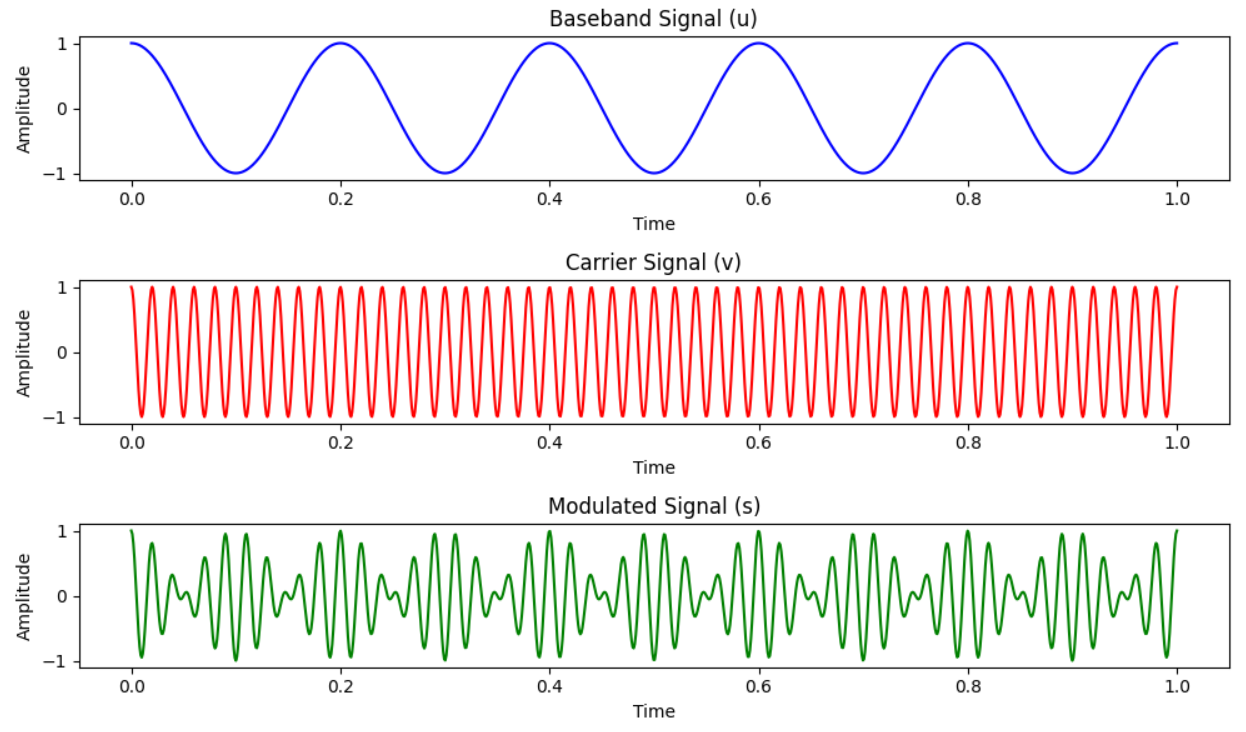
\includegraphics[scale=0.5]{images/AM_mod.PNG}
\caption{Exemple de modulation en amplitude}\label{term1}
\end{figure}

\subsection{Modulation en fréquence}

La modulation en fréquence (\textit{Frequency modulation, FM}) encode les informations dans les caractéristiques temporelles du signal transmis, ce qui la rend plus robuste aux interférences liés à l'amplitude que la modulation AM. La fréquence d'un signal ne peut pas être modifiée par le bruit ou la distorsion. Cepdendant, d'autres types de distortions comme le \textit{frequency drift} (un changement non désiré de la fréquence dans le temps) peuvent affecter la qualité d'un signal modulé en fréquence. Selon l'équation \ref{eq113}, le paramètre à faire varier est $f_c$. Contrairement à la modulation en amplitude, le signal porteur et modulé ne sont pas similaires ($m(t) \neq U_c(t)$). Dans \ref{eq113}, la phase $\phi(t)$ vaut $2 \pi f_ct + \theta_c$ où $\theta_c$ est une constante. Pour déterminer la fréquence instantanée, il faut dériver la phase instantanée c'est à dire :

\begin{equation}\label{eq120}
f_i(t) = \frac{1}{2\pi} \frac{d\phi_i(t)}{dt}
\end{equation}

Ainsi, il est possible de représenter l'accumulation de la phase due à la modulation par l'équation :

\begin{equation}\label{eq121}
U_c(t) = U_c.\cos(2 \pi \int_{0}^{t} f_i(\tau) \, d\tau +  \theta_c)
\end{equation}

\vspace{0.1cm}

Soient $u(t)$ un baseband signal et $v(t)$ un carrier signal, le signal modulé en fréquence $s_{fm}(t)$ est le résultat suivant :

\begin{align}
    u(t) &= \sin(2\pi f_{u}t) \\
    v(t) &= \cos(2\pi f_{c}t + \phi_{c}) \\
    s_{fm}(t) &= \cos\left(2\pi f_{c}t + \Delta f \cdot u(t) + \phi_{c}\right)
\end{align}

\vspace{0.1cm}

Reprennons le même signal en bande de base 
$u(t)$ = $sin(2\pi f_{u}t)$ avec $f_{u}$ = 5 Hz et la même porteuse 
$v(t)$ = $cos(2\pi f_{c}t + \phi_{c})$ où $f_{c}$ = 50 Hz.

\vspace{0.1cm}

La Figure \ref{term2} montre le signal modulé $s_{fm}(t)$ via la modulation en fréquence pour une phase initale du carrier signal $\phi_{c}$ = 0 avec une dérivation en fréquence $\Delta f$ = 5Hz. On remarque la présence d'une constante représentant un décalage de phase. La modulation en fréquence n'est pas détachée de la modulation en phase. Les deux modulations fonctionnent à partir de la phase instantannée $\phi_i(t)$. La modulation en fréquence fait varier linéairement la fréquence instantanée $f_i(t)$ (qui dépent de $\phi_i(t)$ par \ref{eq120}) tandis que la modulation en phase fait varier linéairement la phase instantannée $\phi_i(t)$. Ajouté à cela, $u(t)$ est un sinus, or 

\begin{equation}\label{eq122}
\int_{0}^{t} \sin(2 \pi f \tau \, d\tau) = \frac{1 - \cos(2\pi f t)}{2 \pi f}
\end{equation}

Ce qui implique que le signal modulé a subi un décalage de $\frac{\pi}{2}$ radian car l'identitée trigonométrique indique que :

\begin{equation}\label{eq122}
\cos(x+\frac{\pi}{2}) = \sin(x)
\end{equation}

\begin{figure}[h]
\centering

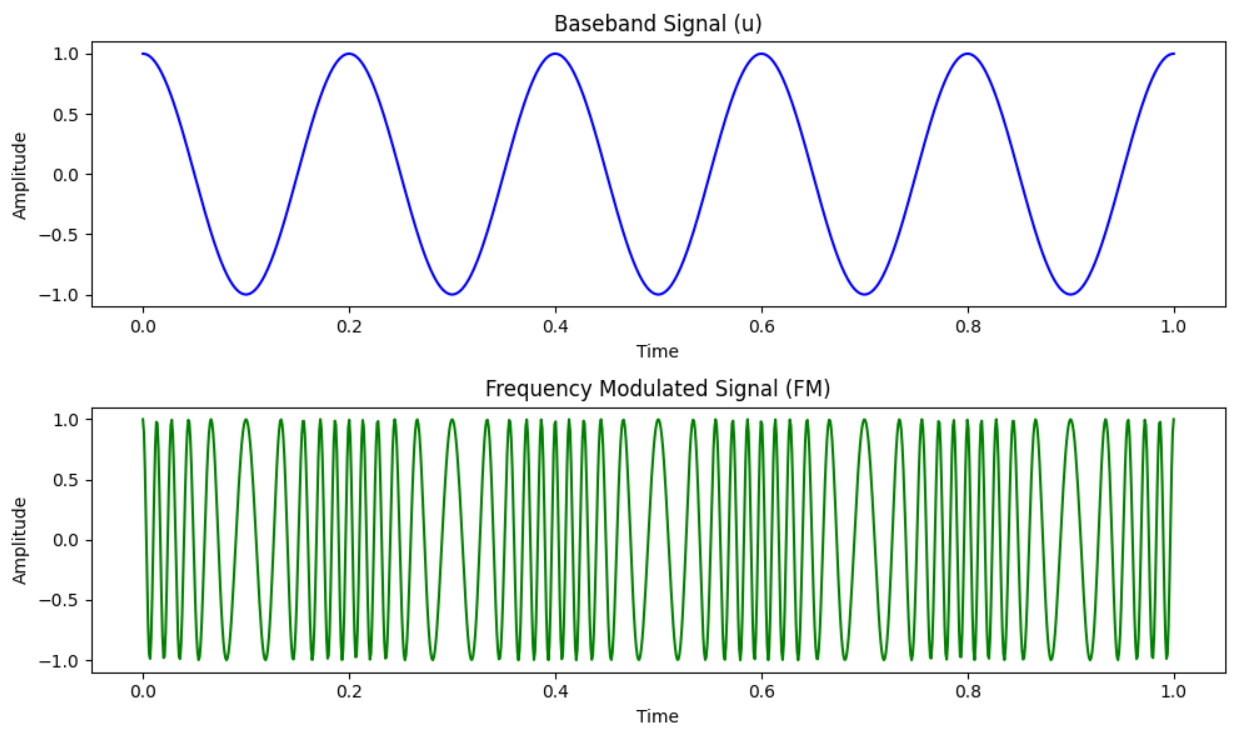
\includegraphics[scale=0.5]{images/FM_mod.PNG}
\caption{Exemple de modulation en fréquence}\label{term2}
\end{figure}

\subsection{Modulation en phase}

La modulation en phase (\textit{Phase Modulation, PM)} permet généralement d'obtenir une meilleur utilisation de la bande passante que les autres modulations car les variations de phase peuvent encoder plus d'informations, ce qui augmente la quantité de données transmises. La modulation en phase est associée à celle en fréquence. En effet les concpets sont liées par leur dépendance à $\phi_i(t)$ . Peu importe l'argument de la fonction de modulation choisi, il n'est plus une fonction linéaire du temps.

Soient $u(t)$ un baseband signal et $v(t)$ un carrier signal, le signal modulé en phase $s_{pm}(t)$ est le résultat suivant :

\begin{align}
    u(t) &= \sin(2\pi f_{u}t) \\
    v(t) &= \cos(2\pi f_{c}t + \phi_{c}) \\
    s_{pm}(t) &= \cos\left(2\pi f_{c}t + K_{p} \cdot u(t)\right)
\end{align}

\vspace{0.1cm}

Prenons par exemple

\vspace{0.1cm}

$u(t)$ = $sin(2\pi f_{u}t)$ avec $f_{u}$ = 5 Hz,

$v(t)$ = $cos(2\pi f_{c}t + \phi_{c})$ où $f_{c}$ = 50 Hz.

\vspace{0.1cm}

La Figure \ref{term3} montre le signal modulé $s_{pm}(t)$ en phase pour une phase initale ddu carrier signal $\phi_{c}$ = 0 avec un index de modulation de phase $K_{p}$ = 8.


\begin{figure}[h]
\centering

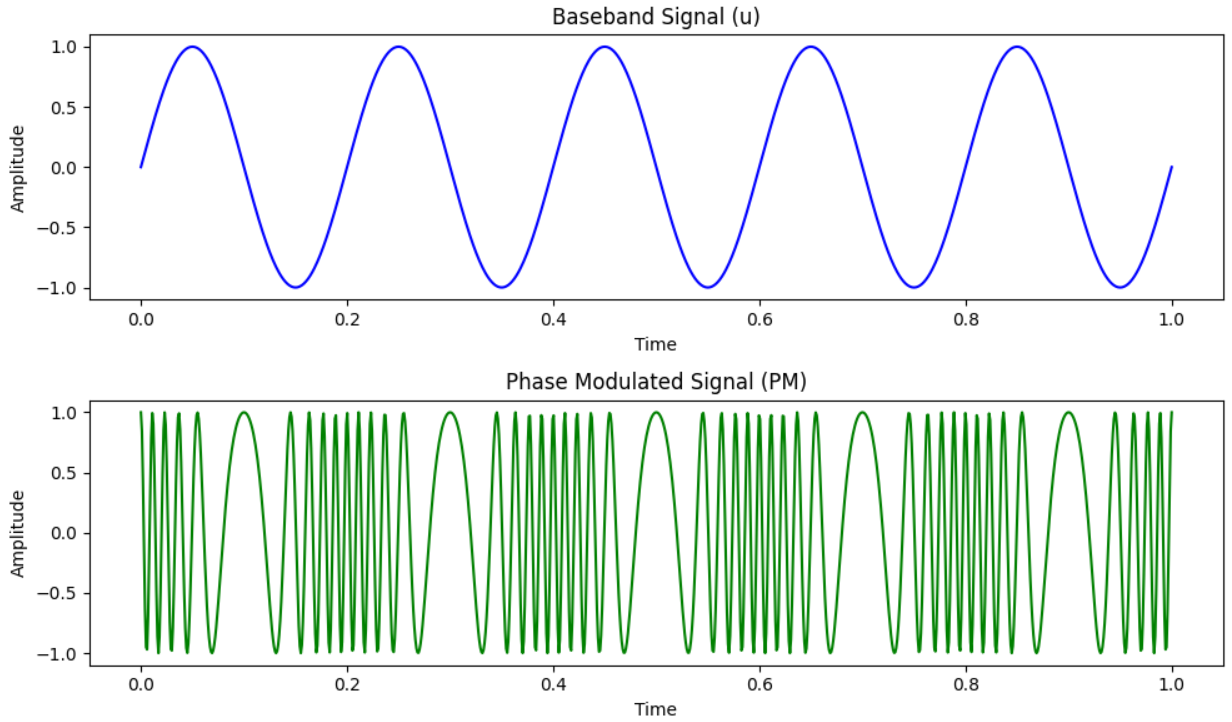
\includegraphics[scale=0.5]{images/PM_mod.PNG}
\caption{Exemple de modulation en phase}\label{term3}
\end{figure}

On constate que pour un signal sinusoidal il est assez difficile de différencier la modulation en fréquence de celle en phase. La différence a lieue à l'emplacement des variations de la vitesse d'oscillation. Pour la modulation en fréquence, on constante que l'oscillation accélère jusqu'à atteindre le maximum quand l'amplitude du signal en bande de base est maximale, et inversément quand l'amplitude est au minimum. Les concepts de modulation de phase et de frénquences sont généralement regroupés sous le terme de modulation angulaire (source : \href{http://www.telecom.ulg.ac.be/teaching/notes/total1/elen008/node39_mn.html}{http://www.telecom.ulg.ac.be/teaching/notes/total1/elen008/node39mn.html})


\subsection{Gestion du bruit}

L'un des attributs cités concerne le bruit. Un signal est toujours affecté de petites fluctuations plus ou moins importantes, et dont les origines peuvent être diverses. Ces perturbations, appelée bruit ou \textit{noise} en télécommunication se définissent par l'altération non souhaitée de l'intégrité d'un signal. Le bruit peut prendre différentes formes, des perturbations essentiellement impulsionnelles engendrées par des commutations de courants ou alors du bruit de fond généré dans les câbles et les composants électroniques en raison
des mécanismes statistiques de la conduction électrique. Il est possible de réduire voir éliminer l'influence des perturbations impulsionelles. En revanche, le bruit de fond est lui irreductible. Tout signal sans bruit n'existe pas, même à l'émission. Il est cependant possible que le bruit devienne invisible si son niveau est très faible. L'attribut SNR est donc un critère de la qualité du signal.


\subsection{Transformée de Fourier}

Les notations sont également reprises du livre \textit{An introduction to analog and digital communication} de S. Haykin\cite{book1}.

\vspace{0.1cm}

Pour effectuer une analyse de signal, sa représentation est capitale. Les Figure 1 et 2 représentent des signaux en fonction du temps écoulé, soit dans le domaine temporel. Il est possible de représenter des signaux selon une autre composante, la fréquence, c'est à dire dans le domaine fréquenciel.

\vspace{0.1cm}

La transformée de Fourier est un outil fondamental utilisé pour analyser et décomposer des signaux complexes en composantes fréquentielles. En transformant un signal dans le domaine temporel en sa représentation dans le domaine fréquentiel, la transformée de Fourier révèle les différentes composantes fréquentielles présentes dans le signal.

\vspace{0.1cm}

Pour les signaux continus, la \textit{CFT} (Transformée de Fourier continue ou juste Tranformée de Fourier) convertit une fonction du temps en fonction de la fréquence en intégrant le signal par rapport aux sinusoïdes de toutes les fréquences possibles. Cette transformation fournit les informations d'amplitude et de phase pour chaque composante de fréquence présente dans le signal. La Transformée de Fourier Continue peut être calculée de la manière suivante :  

\begin{equation}\label{eq11}
G(f) = \int_{-\infty}^{\infty} g(t)e^{-j\omega t} dt
\end{equation}

où : $G(f)$ est la Transformée de Fourier du signal $g(t)$ à la fréquence $f$. $\omega$ représente la fréquence angulaire $(2 \pi f)$.
Il est également possible de revenir dans le domaine temporelle, grâce à la Transformée de Fourier inverse (IFT) :

\begin{equation}\label{eq12}
g(t) = \int_{-\infty}^{\infty} G(f)e^{j\omega ft} df
\end{equation}
Les deux équations \ref{eq11} et \ref{eq12} sont les complexes conjugués l'une de d'autre.

\vspace{0.1cm}

Reprenons la modulation en amplitude de la section \ref{mod}. En utilisant la CFT sur les trois signaux (bande de base, porteuse et modulé) de la figure \ref{term1}, la figure \ref{term8} montre leurs CFT respectives.

\begin{figure}[h]
\centering

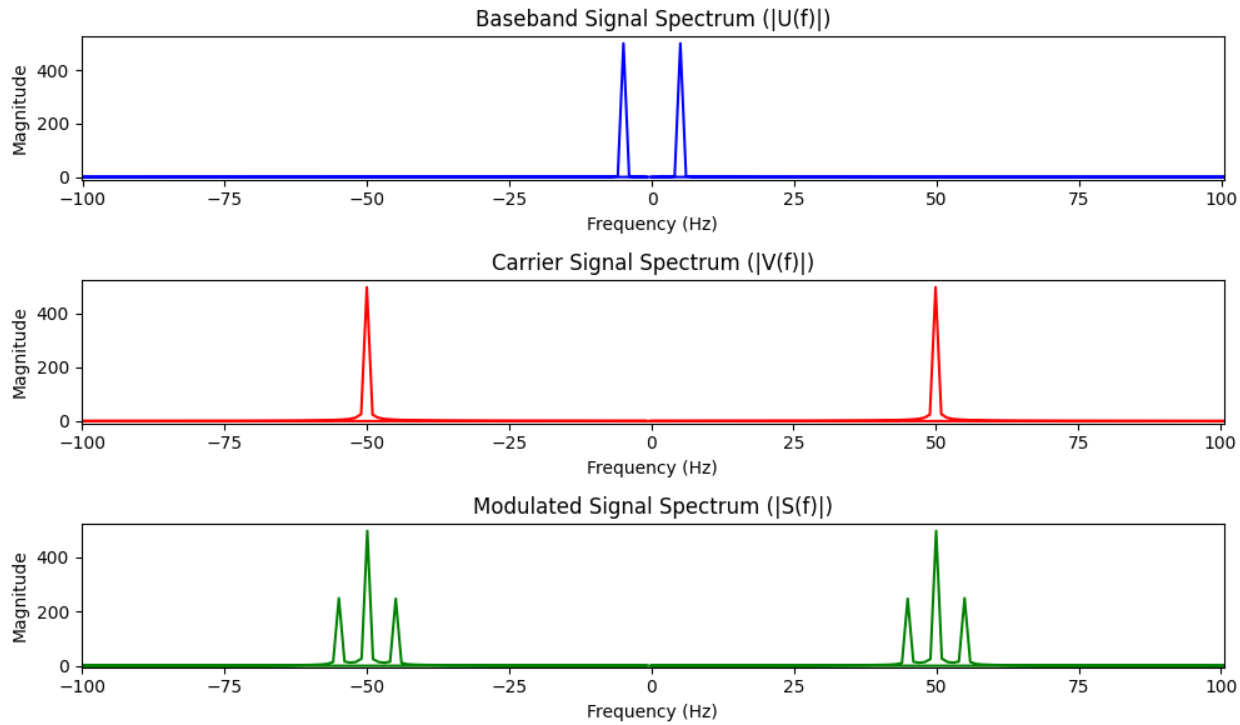
\includegraphics[scale=0.5]{images/CFT.PNG}
\caption{Exemple de CFT}\label{term8}
\end{figure}

La première chose que l'on constate, c'est que pour le singal en bande de base et la porteuse, on observe pour chacun d'entre eux deux pics. Ces pics correspondent à la fréquence des différents signaux (pour rappel $f_u$ = 5Hz et $f_v$ = 50Hz) mais aussi à leur fréquence négatives. Cette duplication est due au fait que la Tranformée de Fourier produit un spectre symétrique par rapport à l'origine (dans notre cas, le centre où la fréquence vaut 0Hz). La CFT d'un signal réel possède deux valeurs (positives et négatives) pour chaques composantes du signal. On constate également que sur la CFT du signal modulé il y a 4 pics. Ces pics sont expliqués par un décalage en fréquence du à la modulation. En effet le troisième signal est un produit de deux signaux, dans le domaine fréquenciel ce produit apparait comme un décalage de la fréquence du signal en bande de base de part et d'autre de la fréquence du signal de la porteuse. C'est le théorème de la modulation. Pour des signaux $u(t)$ et $v(t)$ ayant pour CFT respectives $U(f)$ et $V(f)$, alors leur relation peut être exprimée de la manière suivante :

\begin{equation}
u(t)v(t) = \int_{-\infty}^{\infty} U(f)V(t - f) df
\end{equation}

Ainsi, par l'identité trigonométrique \ref{eq114}, le signal modulé possède un pic à 50 - 5 Hz et à 50 + 5 Hz selon le signal en bande de base. Comme le signal est réel, les mêmes pics sont observés à l'opposé du centre de la symétrie.

\vspace{0.1cm}

Pour les signaux discrets et échantillonnés, la \textit{DFT} (Transformée de Fourier discrète) calcule un ensemble fini de composantes de fréquence. Il est calculé à l’aide d’un nombre fini d’échantillons, ce qui donne des composantes de fréquence discrètes. Il existe un méthode optimisée pour les signaux discrets appelé \textit{FFT (Fast Fourier Transform)}\cite{fft}. Il s'agit d'un moyen plus rapide et moins couteux de calculer la transformée de Fourier, en particulier pour les signaux numériques comportant un grand nombre de points de données. La DFT calcule la transformé de Fourier pour une séquence de N échantillons en $O(N^2$) tandis que la FFT optimise le temps de calcul en $O(N log N)$ pour la même séquence. Il existe diverses variante de la FFT (par example le Cooley-Tukey FFT\cite{fft1}) ce qui peut légèrement faire varier les performances dépendant de l'algorithme utilisé. Les logiciels utilisés pour l'analyse de signaux dans la section \ref{fft} utilisent des algorithmes de FFT pour leurs affichages dans le domaine fréquenciel.

\newpage

\section{LoRa}

\textit{LoRa} (Long Range) est une technologie de communication sans fil qui permet de transmettre des données sur de longues distances avec une faible consommation d'énergie. Elle a été développée par la société française Cycleo (qui a été racheté par Semtech en 2012 \cite{sitesemtech}) et est maintenant gérée par la fondation LoRa Alliance, qui regroupe plusieurs entreprises et organisations du monde entier. Toutes les informations de base concernant LoRa sont disponibles sur le site LoRa Alliance (\href{https://lora-alliance.org}{https://lora-alliance.org})

\begin{figure}[h]
\centering

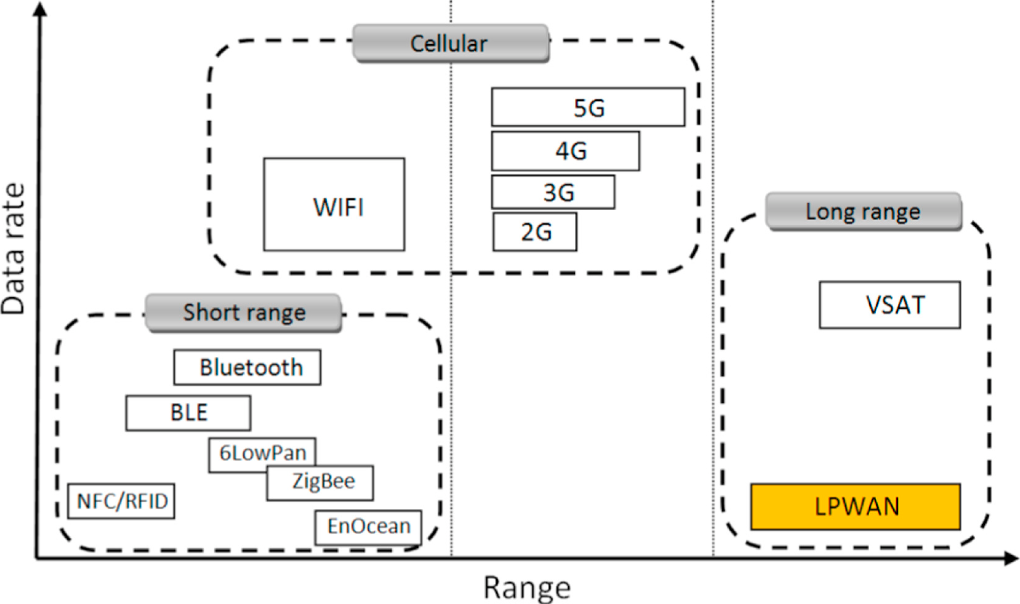
\includegraphics[scale=0.5]{images/lpwan.png}
\caption{Spectre des technologies sans fil}\label{term101}
\end{figure}


LoRa est principalement utilisée dans l'IoT. Elle se distingue par sa portée étendue, qui peut atteindre plusieurs kilomètres en milieu urbain et plusieurs dizaines de kilomètres en milieu rural, ainsi que par sa faible consommation d'énergie, qui permet de prolonger la durée de vie des appareils connectés. Lora fait partie des technologies appelées \textit{LPWAN (Low Power Wide
 Area Network)}. La figure \ref{term101} montre le spectre des technologies sans fil actuelles. Cette image est reprise du document \textit{A comparative study of LPWAN technologies for large-scale IoT deployment}\cite{lpwan1}. Une longue portée avec un puissance limitée induit un débit de transmission plus faible que les autres technologies sans fil (le Wifi, la 4G, Bluetooth etc).

\vspace{0.1cm}

LoRa utilise une bande de fréquences qui varie selon les régions du monde où LoRa est déployée :

\vspace{0.1cm}

\begin{itemize}
\item en Europe, la bande de fréquences autorisée est comprise entre 863 et 870 MHz, ce qui correspond à l'\textit{ISM radio band}, une bande dédiée aux recherches qui ne nécessite pas de license d'émission.
\item aux États-Unis, elle se situe entre 902 et 928 MHz,
\item en Chine, la fréquence autorisée varie entre 779 et 787 MHz,
\item les régions restantes ont elles aussi une fourchette unique.
\end{itemize}

\vspace{0.1cm}

La technologie LoRa utilise la modulation appelé \textit{Chirp Spread Spectrum Modulation} (CSS). La modulation CSS utilise un signal chirp, c'est à dire un signal modulé linéairement en fréquence. Ce signal a une amplitude constante mais balaie tout le spectre de la bande passante de manière linéaire dans une période de temps définie. Cette technique de modulation est détaillée à la section \ref{css}

\vspace{0.1cm}

La technologie LoRa utilise également une technique de multiplexage en temps partagé (\textit{Time Division Multiple Access}) pour permettre à plusieurs appareils de partager la même bande de fréquences de manière à maximiser l'utilisation de la capacité de transmission. Elle utilise également une technique de diffusion de données (\textit{multicast}) pour envoyer les mêmes données à plusieurs appareils simultanément, ce qui permet de réaliser des économies de bande passante et d'énergie (source : \href{https://resources.lora-alliance.org/technical-trainings/lorawan-device-to-device-multicast-communications}{LoRa Alliance : https://resources.lora-alliance.org/technical-trainings/lorawan-device-to-device-multicast-communications})

\vspace{0.1cm}

En plus de sa portée étendue et de sa faible consommation d'énergie, LoRa se distingue par sa sécurité de transmission via LoRaWAN, qui est assurée grâce à l'utilisation de codes de sécurité uniques et à la possibilité de chiffrer les données transmises. Lora n'est pas exclusivement lié au protocole LoRaWAN. Ce protocole est décrit en détails à la section \ref{lorawan}. Si LoRa opère à un niveau plus bas que la plupart des protocoles réseau, LoRaWAN via son infrastructure (notament les \textit{gateways}) permet entre autre aux appareils LoRa de pouvoir servir d'intermédiaire avec différents protocoles et d'être compatibles avec un grand nombre de protocoles de communications comme \textit{TCP/IP (transport layer protocol), HTTP (hypertext transfer protocol ou MQTT(message queuing telmetry transport)}.

\vspace{0.1cm}

Toutes ces  particularités font de LoRa une technologie complémentaire à celles déja existantes plutot que rivale.
LoRa se compose de deux éléments principaux : la couche physique de la technologie et LoRaWAN, la couche MAC (\textit{Media Access Control}), une sous couche de la couche liaison de données dans le modèle OSI (\textit{Open Systems Interconnection}). La couche physique de LoRa gère la fréquence radio ainsi que la modulation. LoRaWAN gère les aspects réseaux comme la sécurité, la propagation, l'adressage et la sécurité.

\subsection{Couche physique de LoRa}

\subsubsection{Découpage de la couche physique}

\begin{figure}[h]
\centering

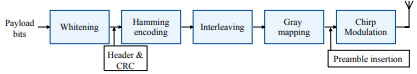
\includegraphics[scale=1]{images/physical_lora_rx.PNG}
\caption{Etapes de la transformation des données dans un émetteur LoRa\cite{loraphy}}\label{term4}
\end{figure}


Les étapes de la conception de l'envoi de données dans la couche physique de LoRa sont montrés dans la figure \ref{term4}. Cette analyse a été faite en \textit{Reverse Engeneering} par Alexandre Marquet, Nicolas Montavont et Georgios Z. Papadopoulos \cite{lorareverse}. Le rétro engineering consiste à analyser un produit ou un système afin de comprendre comment il fonctionne ou d'identifier ses principes de conception. Dans le contexte de LoRa, le reverse engineering examine la technologie derrière LoRa afin de comprendre ses principes de base et sa conception. Les principales étapes de la conceptions de la couche physique LoRa sont les suivants :

\vspace{0.1cm}

\begin{itemize}
\item le blanchiment de canal (\textit{channel withening)}.
Cette technique consiste à utiliser une transformation aléatoire ou pseudo-aléatoire des données avant de les transmettre, de manière à répartir le spectre des fréquences de la transmission sur une large gamme de fréquences. C'est une technique mathématique qui consiste a effectuer une transformation linéaire des données avec une matrice de covariance en un nouveau set de données. Le but du blanchiment est de réduire la corrélation entre les différentes composante fréquencielles et assurer que le signal possède une puissance similaire tout le long de son spectre.
\item Le codage de canal (\textit{channel coding}) est une technique utilisée dans les systèmes de communication sans fil pour améliorer la robustesse et la fiabilité de la transmission des données. Dans le cas de LoRa, le codage de canal utilise le \textit{Forward Error Correction (FEC)} pour corriger les erreurs causées par du bruit. La méthode FEC ajoute de l'information redondante sur les données.
\item Le mélange(\textit{interleaving}) suit le codage de canal.  
Cette technique consiste à réarranger les bits ou les symboles de données en les dispersant sur plusieurs canaux (ici on fait référence à des streams ou a des bandes de fréquences spécifiques plutôt qu'à des canaux physiques). Cela permet de réduire l'impact de \textit{burst errors}, des erreurs consécutives.
\item Le \textit{Gray mapping}. Le code de Gray est une méthode d'ordonnancement de symboles. Le principe de cette méthode est que dans la séquence ordonnée, chaque symbole ne diffère du précedent que d'un seul bit. Utiliser le code de Gray permet de réduire les erreurs dues au bruit ou aux interférences. Les erreurs les plus probables sont celles en deux symboles voisins, soit un bit d'erreur.
\item La modulation CSS est l'étape principale de LoRa. En effet, les étapes précédentes sont communes à de nombreuses technologies, mais la particularité de LoRa provient de la modulation. Cette étape est détaillée dans la section \ref{css}.
\end{itemize}

\vspace{0.1cm}

Chacune des étapes décrites doit être inversément réalisée pour le récepteur. Ainsi pour la récupération de données à l'arrivée, l'appareil récepteur gère la démo \\ dulation, le déblanchiment, le démellement et le décodage.

\subsubsection{Modulation CSS}\label{css}

Le principe de la modulation LoRa est détaillé en profondeur dans l'article \textit{Frequency Shift Chirp Modulation: The LoRa Modulation}\cite{loraCSS} de Lorenzo Vangelista.

\vspace{0.1cm}

La modulation LoRa repose sur le principe de \textit{Frequency Shift Chirp Modulation (FSCM)}, qui est une combinaison de la modulation \textit{Frequency Shift Keying (FSK)} et \textit{Chirp Spread Spectrum (CSS)}.
La modulation CSS étale le signal sur une large bande de fréquences tandis que la modulation FSK décale la fréquence périodiquement dans le temps. Le signal modulé est composé de chirps. Un chirp est un signal dont la fréquence change en continue tout en conservant une amlitude constante. Il existe deux types de chirps : les $upchirps$ et $downchirps$.
Dans un upchirp la fréquence augmente avec le temps tandis que dans un downchirp la fréquence diminue. Soit $s_{chirp}(t)$ un signal chirp avec

\begin{equation}\label{eq3}
s_{chirp}(t) = sin(2\pi(f_0 + (\frac{f_1 - f_0}{2T_s})t)t)
\end{equation}

alors la figure \ref{term5} montre $s_{chirp}$ en fonction du temps où $f_0$ = 10Hz, $f_1$ = 100Hz et $T$ = 1 seconde. On observe que le signal oscille de plus en vite plus vite au fur et à mesure que le temps augmente.

\begin{figure}[h]
\centering

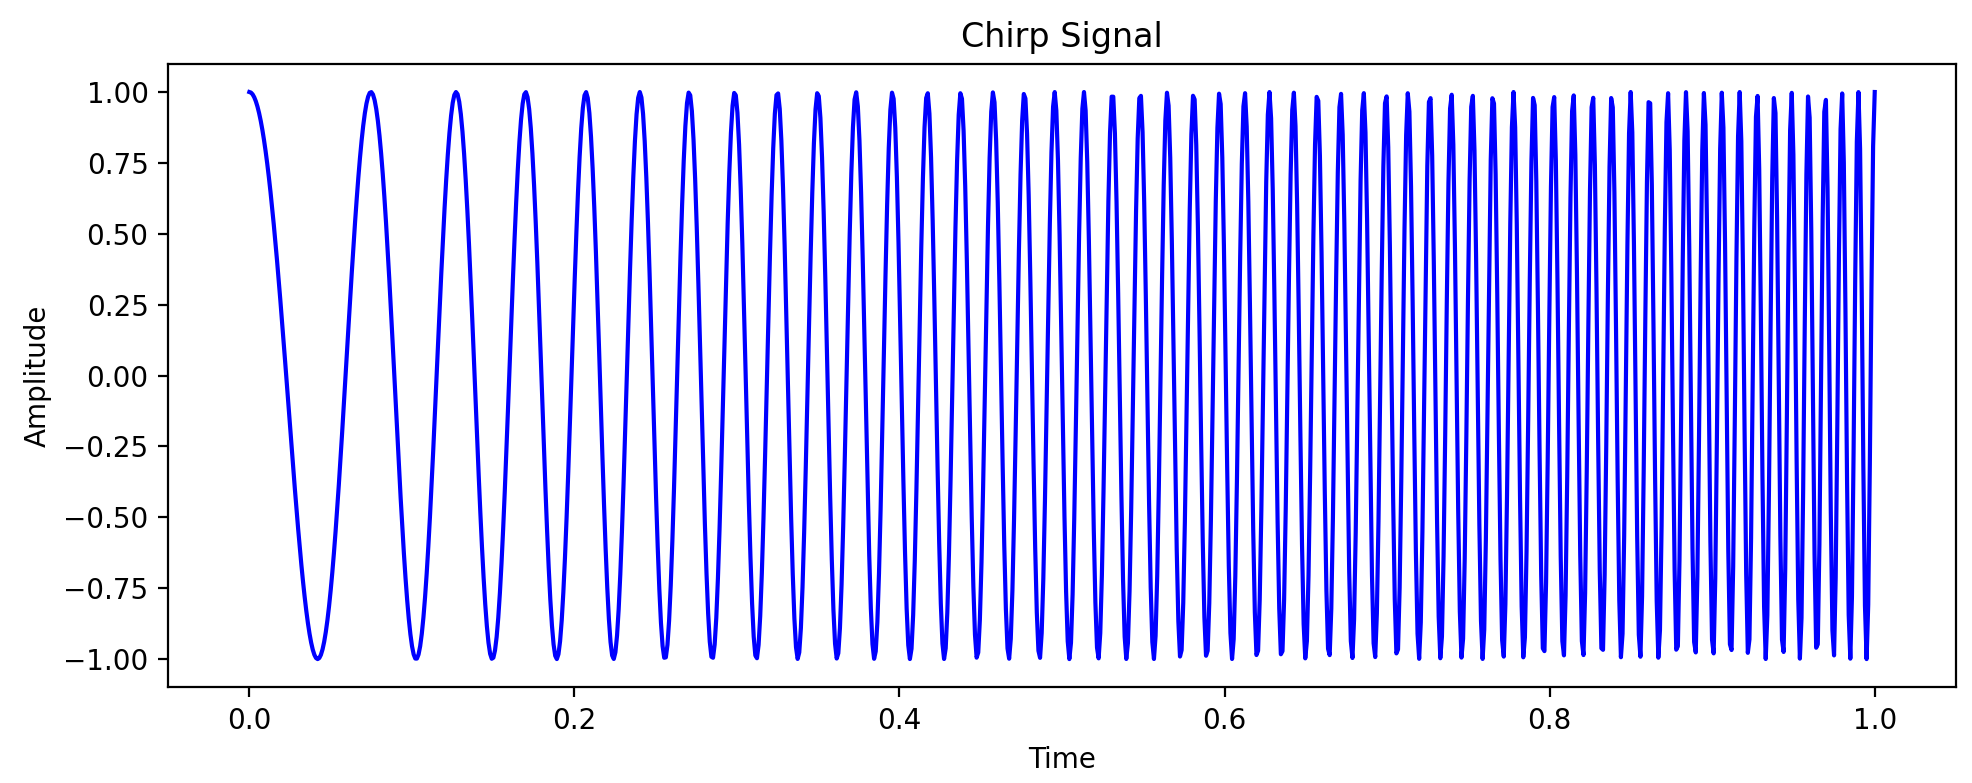
\includegraphics[scale=0.18]{images/CSSupchirp.png}
\caption{Example d'un upchirp}\label{term5}
\end{figure}

\vspace{0.1cm}

Supposons que la bande passante du canal soit $\beta$, LoRa impose qu'un échantillon soit transmis tout les $T$ = $\frac{1}{\beta}$. Un symbole $s(nT_s)$ est envoyé a l'entré de la modulation tout les $T_s$ = $\frac{2^{SF}}{B}$ où \textit{SF (spreading factor)} est le facteur d'étalement. le symbole $s(nT_s$) est un nombre réel formé en utilisant un vecteur de chiffres binaires du facteur d'étalement. Les valeurs de SF pour LoRa sont comprises entre 7 et 12. Lora utilise donc au total $2^{SF}-1$ symboles. L'onde transmise en bande de base pour une durée $T_s$ pour un certain $s(nT_s)$ vaut :

\begin{equation}
c(nT_s + kT) = \frac{1}{\sqrt{2^{SF}}} e^{j2\pi ((s(nT_s) +k )mod 2^{SF})kT \frac{\beta}{2^{SF}}}
\end{equation}
pour $0 \leq k \leq 2^{SF}-1$ et $0 \leq s(nT_s) \leq 2^{SF}$.
Le signal modulé est donc une onde composée de chirps. Chaque fragment de l'onde diffère de l'onde possèdant une fréquence initiale à 0, par un décalage de fréquence $s(nT_s)$. Cette caractéristique est la raison de l'appellation FCSM.


\subsubsection{Spreading factor}

LoRa permet d'envoyer des paquets sur une longue distance à faible puissance. Selon l'environnement dans lequel les appareils LoRa sont présents, il peut être utile de pouvoir ajuster certaines capacités.

\vspace{0.1cm}

Le facteur d'étalement permet de déterminer le taux de variation de fréquence pour un signal. Modifier le spreading factor ajuste diffé \\ rentes propriétés de la communications (source : The Thing Network\cite{thethingsnetworkSF}). Par exemple, si on augmente le spreading factor, les quatre conséquences principales sont :

\vspace{0.1cm}

\begin{itemize}
\item l'augmentation de la portée. En effet augmenter le SF réduit le bitrate et augmente le \textit{processing gain} (l'augmentation de la puissance du signal atteint en l'étalant sur une plus large bande).
\item Augmentation de la résistance aux interférences. Comme le signal est étalé sur une bande plus large, il y a moins de risque de subir des interférences.
\item Plus petit débit de données. Le spreading factor contrôle le taux de chirp, et du coup la vitesse de transmission de donnée. Augmenter le speading factor signifie ralentir la vitesse d'émission des chirps. Pour chaque augmentation du spreading factor, le taux de transmission de donnée est réduit de moitié.
\item Plus grande consommation. Les données transmises à un taux plus faible, la durée de transmission est donc plus longue ce qui prolonge le cout pour envoyer l'information.
\end{itemize}

Diminuer le spreading factor engendre l'effet inverse \cite{thethingsnetworkSF}.


\subsubsection{Structure d'un paquet LoRa}\label{packetlora}

\begin{figure}[h]
\centering

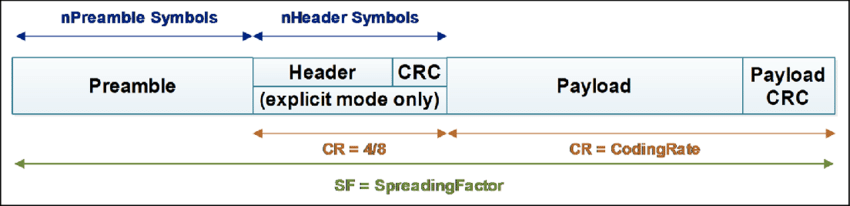
\includegraphics[scale=0.4]{images/lorapacket.png}
\caption{Structure d'un paquet Lora\cite{lorapacket}}\label{term6}
\end{figure}


La figure \ref{term6} montre la structure d'un paquet Lora. Un paquet LoRa contient 3 parties différentes \cite{loraphy} :

\vspace{0.1cm}

\begin{itemize}
\item Le \textit{preamble}. La première partie du paquet, composée d'un nombre variable d'upchirps. La valeur par défaut est fixée à 8 upchirps minimum. L'émetteur radio ajoute à cela un peu plus de 4 symboles (4,25), qui contiennent l'identificateur réseau ainsi que deux downchirps de synchronisation de fréquence. Ceci fixe le préambule à 12,25 symboles.
\item Le \textit{header} du paquet. Les informations sur la taille du paquet, le code rate, la présence d'un CRC (\textit{cyclique redundancy check}) et la checksum sont incluses dans l'en-tête.
\item Le \textit{payload}. La dernière partie du paquet qui contient les données à transmettre. La taille maximale du payload est de 255 octets. En plus des données, le payload peut également contenir un CRC pour la détection d'erreurs. La longueur du CRC est par défaut de 16 bits.
\end{itemize}

\newpage
\subsection{LoRaWAN}\label{lorawan}

LoRaWAN est un protocol de type \textit{Low Power Wide Area Network (LPWAN)} conçu pour la communication longue portée. Ce protocole opère avec la technologie LoRa et lui fournit une infrastructure capable de maintenir une communication à longue portée et à faible cout dans l'IoT.

\subsubsection{Aspects généraux de la technologie}

Le coeur de LoRaWAN réside dans la gestion de l'énergie, permettant aux appareils de fonctionner avec une consommation d'énergie minimale, prolongeant leur durée de vie tout en garantissant une fonctionnalité à long terme. Elle est également efficace dans différents environnements. Le signal est capable de pénétrer diverses terrains et structures. Cela rend la technologie efficace aussi bien milieu rurale qu'urbain.
Le déploiment d'une infrastructure LoRa ne nécessite pas de license, et son réseau peut être public ou privé.

\vspace{0.1cm}

LoRaWAN opère sur une bande de fréquence qui ne nécessite pas de license d'émition, par exemple sur la bande ISM pour \textit{Industrial, Scientific, and Medical}. Les bandes ISM, (868 MHz en Europe ou 915 MHz aux USA) sont disponibles pour l'utilisation de différentes technologies, incluant LoRaWAN.

\vspace{0.1cm}

LoRaWAN possède des capacités de géolocalisation, permettant au réseau de détecter et de localiser précisément les appareils au sein de son domaine. LoRaWAn utilise différentes méthodes pour localiser ses appareils comme \textit{Received signal strengh indication (RSSI)}, \textit{Time difference on Arrival (TDOA)}, une triangulation ou alors une combinaison de plusieurs des méthodes. Certaines de ses méthodes seront détaillées dans la section \ref{identification}

\vspace{0.1cm}

LoRaWAN utilise des protocoles de sécurité \textit{end-to-end}, aussi bien dans un réseau public intégré que dans un réseau privé. L'architecture LoRaWAN (décrite en détails dans la section \ref{topolora}) contient plusieurs couches de sécurité. Au niveau des \textit{end devices}, une routine d'identification est imposée avant l'accès au réseau. Seul les appareils de confiance sont donc autorisés à communiquer. Ensuite, une fois la communication commencée, les données sont chiffrées avant d'être transmises dans le réseau. Le framework sécuritaire de LoRa ne se limite pas à l'autentification et au chiffrement. LoRaWAN gère également les mise à jour en continu par les airs, ainsi qu'une supervision continue sur d'éventuelles intrusions. Les caractéristiques générales de LoRaWAN sont disponibles sur le site The Thing Network (\href{https://www.thethingsnetwork.org/docs/lorawan/}{https://www.thethingsnetwork.org/docs/lorawan/}).

\vspace{0.1cm}

Avec toutes ces caractéristiques, LoRaWAN s'est développé dans de nombreux domaines aussi bien environementaux qu'industriels. Les principales utilisations de LoRaWAN actuelles sont les suivantes (liste des applications : \href{https://www.semtech.com/lora/lora-applications}{https:// \\ www.semtech.com/lora/lora-applications}):

\vspace{0.1cm}

\begin{itemize}

\item la surveillance environementale en général \cite{lorauc1}. LoRaWAN peut être déployé pour surveiller des niveaux de températures, d'humidité, de bruits ou encore d'autres paramètres dans n'importe quel milieu. Une compagnie Hollandaise, Sensoterra (\href{https://www.sensoterra.com/technology/global-lorawan-networks/}{https://www.sensoterra.com/techno \\ logy/global-lorawan-networks/}), utilise notamment LoraWan pour surveiller la qualité des sols.
\item Les \textit{smart cities} \cite{lorauc2}. LoRaWAN est actif sur différents aspects comme la gestion intelligente de l'éclairage, la gestion des déchets, la surveillance, etc.
\item L'embarqué industriel \cite{lorauc3}. La maintenance et la surveillance de matériel et de l'équipement peut être gérée par LoRaWAN. TataSteel (\href{https://consulting.tatasteel.com/our_expertise/plant-infrastructure-and-logistics/}{https://cons \\ ulting.tatasteel.com/ourexpertise/plant-infrastructure-and-logistics/}), une compagnie indienne, utilise LoRaWAN pour ces équipements industriels.
\item La prévention de catastrophe naturelle. Que ce soit en prévision\cite{lorauc41} ou après\cite{lorauc43} d'éventuelles catastrophes naturelles, la longue portée et la surveillance en temps réel sont des atoux cruciaux pour ce genre d'évènement.
\end{itemize}

\vspace{0.1cm}

Cependant, toutes ses caractéristiques entrainent un certain nombre de limitations. La restriction de la fréquence en fonction de la région peut rendre le déploiment d'une même infrastructure à différents endroits dans le monde plus difficile. Cela peut aussi entrainer des problèmes de compatibilité entre régions, notament pour des chaines logistiques ou d'approvisionement qui en traversent plusieurs.

\vspace{0.1cm}

Une faible consommation de puissance avec une grande portée a un impact sur la taille et la vitesse de l'information. La taille du payload d'un message est limitée entre 51 et 241 octets. La vitesse de transmission est également peu élevée, atteignant un maximum de 5.5kbps sur une largeur de bande de 125kHz pour un facteur d'étalement SF = 7.

\vspace{0.1cm}

La communication au sein d'un réseau LoRaWAN se fait en grande partie de manière asynchrone. La synchronisation dépend de la classe de l'appareils, qui est détaillé dans la section \ref{topolora}. C'est un avantage pour maintenir une grande autonomie de batterie pour les appareils. LoRaWAN possède un système pour limiter les collisions entre messages si plusieurs appareils communiquent simultanénent. Ce système est basé sur une combinaison entre \textit{Listen before talk (LBT)} et des delais aléatoires\cite{loracolision}. Il est néamoins possible que dans un environement très dense des collisions puissent encore se produire. La communication asynchrone et le système d'évitement de collision entrainent une augmentation du temps entre les envois et la réception de messages.

\subsubsection{Topologie de LoRaWAN}\label{topolora}

\begin{figure}[h]
\centering

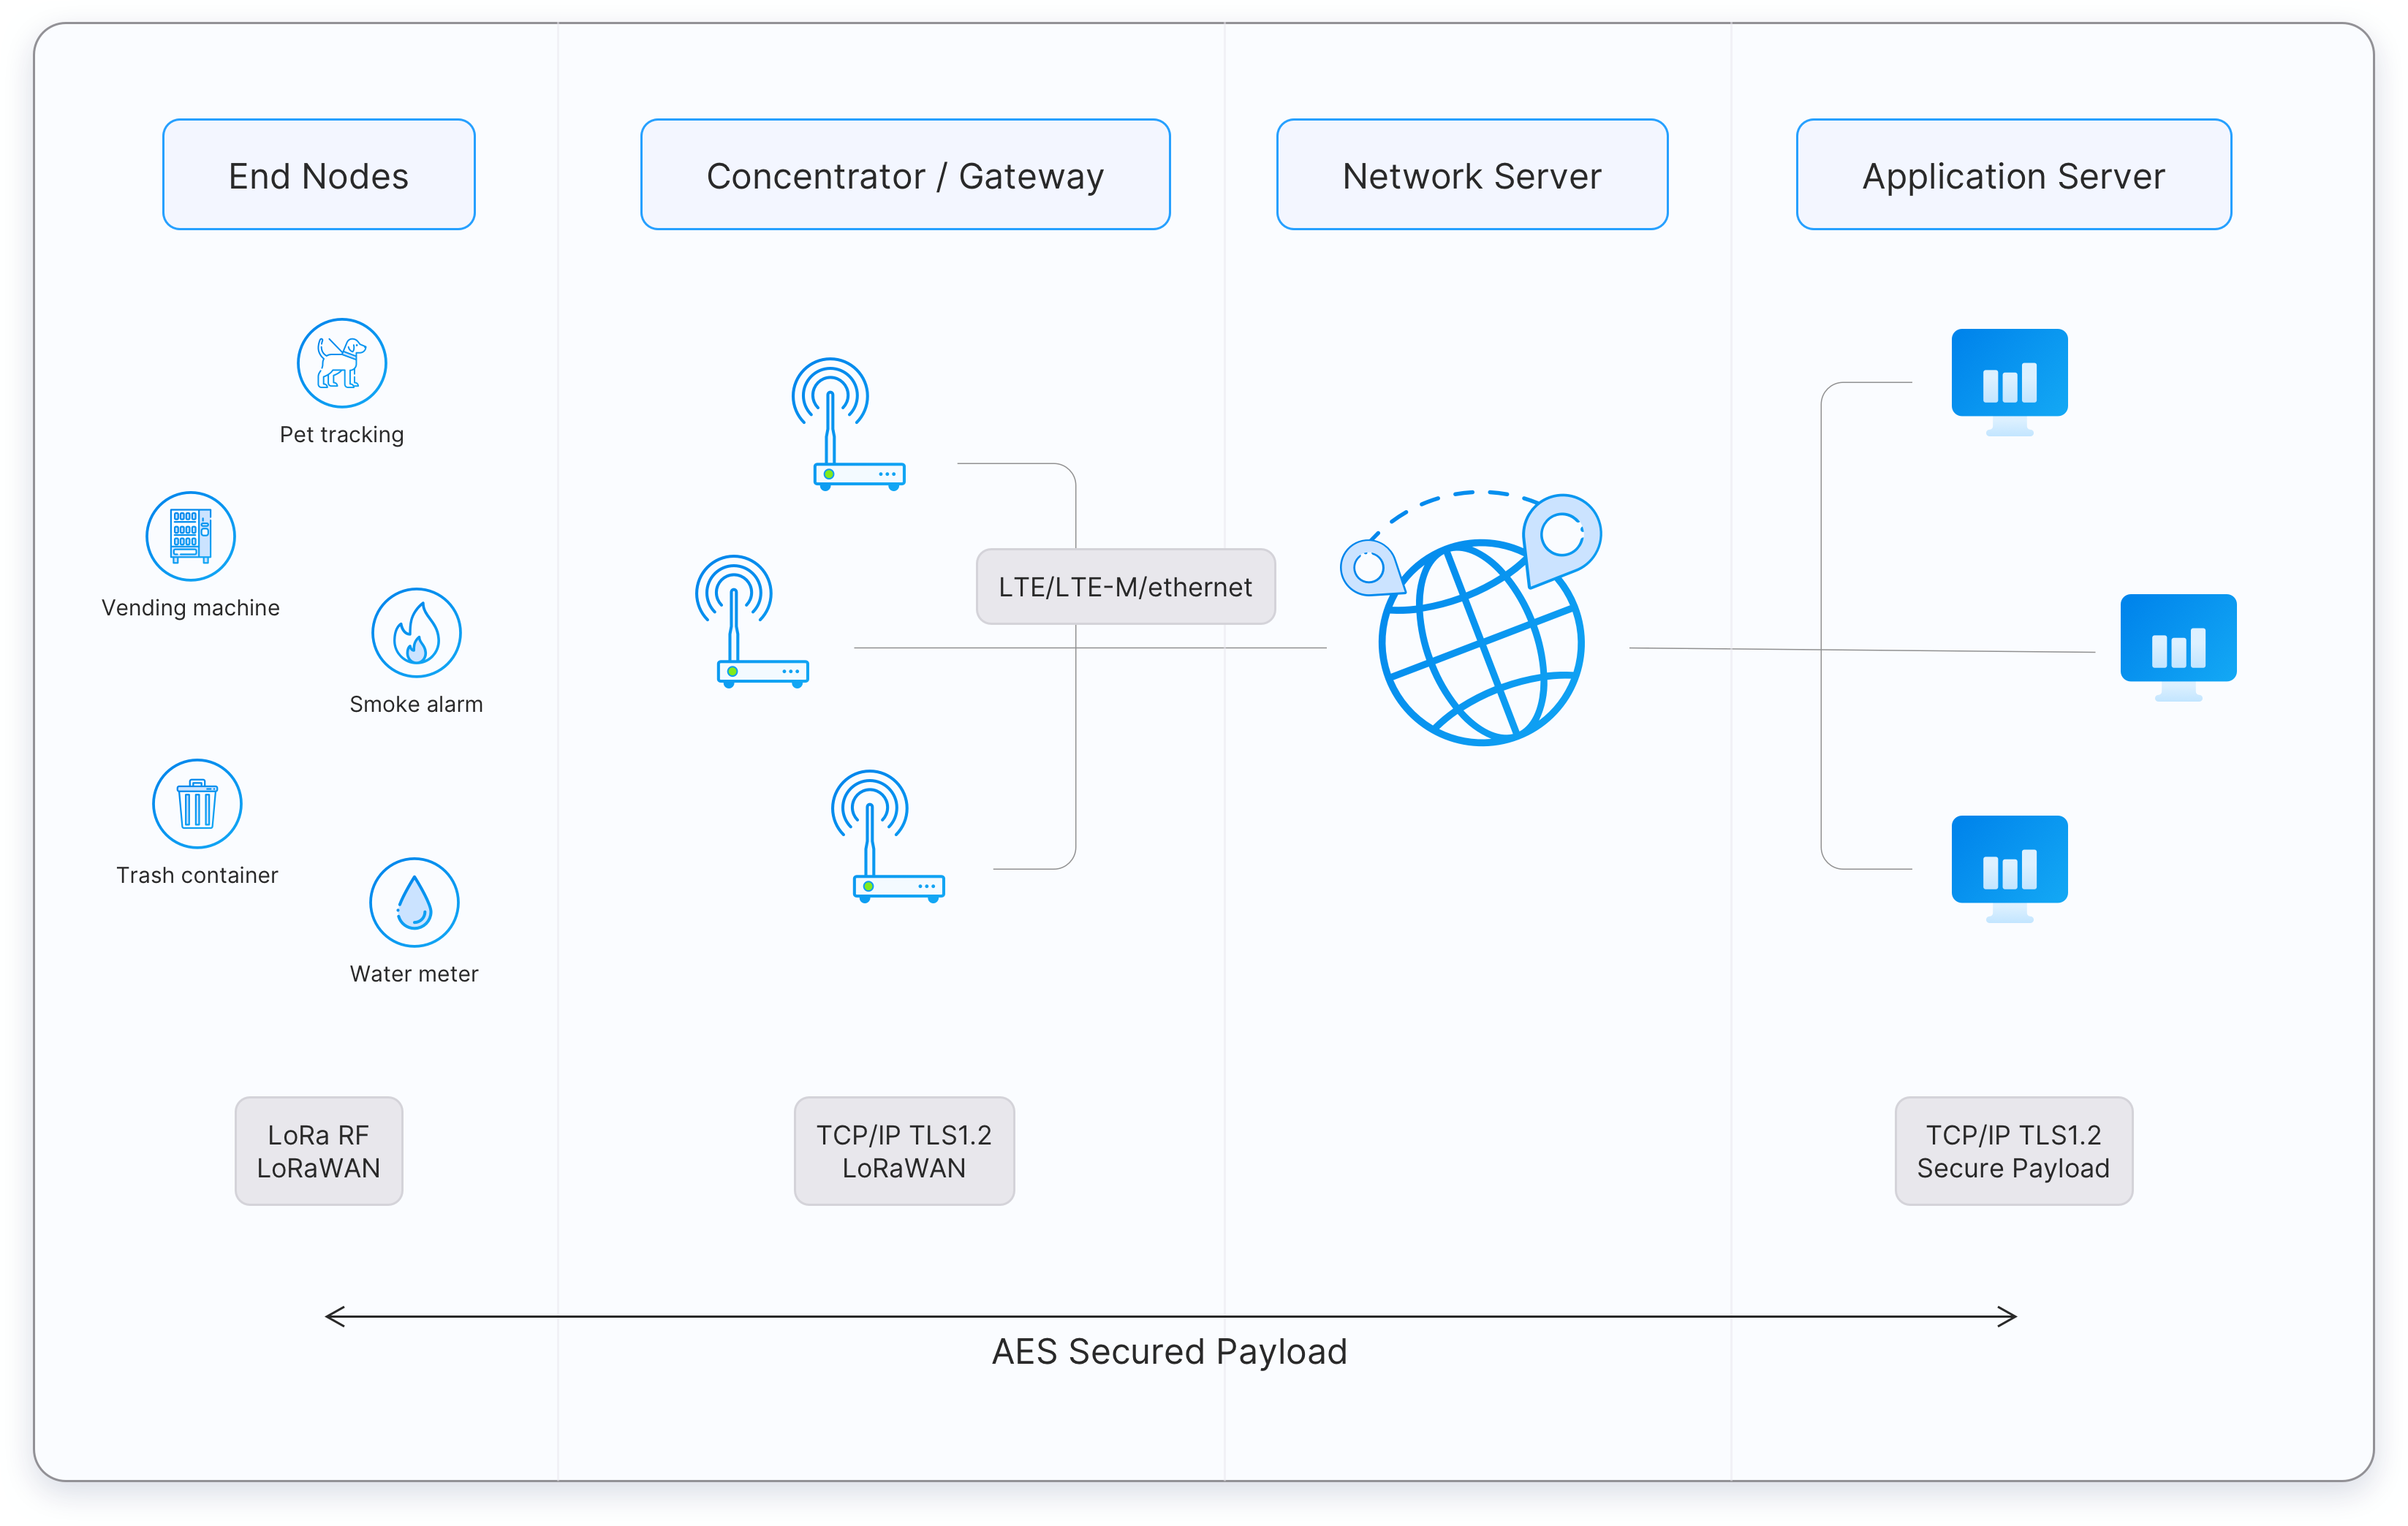
\includegraphics[scale=0.1]{images/architecture.png}
\caption{Topologie de l'infrastructure LoRaWAN (source : \href{https://www.thethingsnetwork.org/docs/lorawan/architecture/}{The Thing Newtork})}\label{term7}
\end{figure}

La figure \ref{term7} montre les 4 types d'appareils qui composent la topologie d'un infrastrucure LoRaWAN.
Les end devices sont les noeuds qui collectent les informations à envoyer à travers le réseau. Ils sont catégorisés en trois sous classes : A, B et C. Les appareils de classe A sont les plus économes en énergie. Ils ont été créés pour conserver leur énergie et communiquent exclusivement en comunication asynchrone. Les appareils de classe A écoutent les messages provenant des serveurs uniquement après avoir eux-même transmis un message. Les appareils de classe B sont assez similaires à ceux de classe A, mais sont occasionellement synchronisés avec les serveurs du réseau. Ils possèdent des capacités supérieures de réception leur permettant de se synchroniser avec le scheduler des serveurs, ce qui augmente considérablement l'efficacité du temps de réponses dans le réseau. Finalement, les appareils de classe C sont en écoute permanente de messages provenant des serveurs. Ils sont les plus réactifs mais également les plus énergivores. Les end devices sont donc classés selon deux paramètres : leur réactivité et leur consomation d'énergie. En fonction de leur classe, ils ont également la possibilité de recevoir des messages server après avoir transmis de l'information. L'envoie d'un message d'un end devices vers les serveurs est appelé \textit{uplink message} et l'envoie d'un message depuis les serveur vers les end devices est appelée \textit{downlink message}.

\vspace{0.1cm}

Les gateways jouent le role d'intermédiaire entre les end devices et le serveur réseau. Ils reçoivent les transmissions depuis les end devices dans leur zone de couverture
et forwardent les messages vers le serveur réseau. Les gateways peuvent écouter plusieurs fréquences simultanénent (\textit{multichanneling}) là où les end devices n'écoutent qu'une seule fréquence. Les gateways gèrent la communication radio avec les end devices en utilisation la modulation de LoRa.

\vspace{0.1cm}

Le serveur réseau est la composante centrale de l'infrastructure. Il gère tout le réseau, que ce soit les données reçues des gateays, l'identification et l'activation des end devices dans le réseau, le routing ou encore l'adapation du data rate. Le serveur réseau supervise également l'aspect sécurité au sein du réseau en gèrant les clés de chiffrement et les protocoles de sécurité.

\vspace{0.1cm}

Le serveur application de LoRaWAN reçoit les données forwardées depuis le serveur réseau. C'est l'interface entre le réseau de LoRaWAN et les différents services ou applications d'utilisateurs finaux. Les utilisateurs intéragissent avec le serveur d'application pour n'importe quelle action à effectuer sur le réseau ou pour la récupération de données du réseau. Les données reçues par le serveur réseau sont traduites par le server d'application avant d'être interprétée par l'utilisateur final.

\subsubsection{Sécurité}

La sécurité dans l'architecture LoRaWAN se concentre sur trois axes principaux :

\begin{itemize}
\item l'authentification : qui communique avec qui.
\item L'intégrité : les données ne sont pas altérées entre l'émetteur et le recepteur.
\item La confidentialité : les données ne sont visibles par personne au sein du réseau hormi l'émetteur et le récepteur. 
\end{itemize}

\vspace{0.1cm}

La sécurité repose sur le chiffrement des données. Les données sont chiffrées en utilisant l'algorithme de cryptographie AES (\textit{Advanced Encryption Standard}). La taille des clés est de 128 bits. Ce choix est motivé par un équilibre entre une sécurité suffisante et une consommation réduite des ressources\cite{loraes}.

\vspace{0.1cm}

Il y a deux types de clés utilisées dans LoRaWAN. La \textit{root key} est la clé partagée entre un end device et le serveur réseau. Cette clé est utilisée pour l'authentification initiale et l'établissement d'une communication entre deux éléments du réseau. Cette clé n'est jamais transmise par les airs, elle est stockée dans un \textit{join server}. Un join server est un server dédié au contenu sensible à l'activation du matériel dans un réseau LoRaWAN. Il authentifie le réseau et les application du servers. Il gère les root keys. il génère également le second type de clés de LoRaWAN, les \textit{session keys}.

Les session keys sont des clés générées dynamiquement par le join server et utilisées durant l'échange de données pendant une session. Il y a deux session keys différentes, la \textit{AppSKEY} pour le chiffrement des payloads d'application, et la \textit{nwkSKEY} pour les fonctionalités du réseau (le chiffrement à la couche MAC, les vérifications d'integrité, etc).

\subsubsection{Session}

L'établissement d'une session entre un end devices et le réseau LoRaWAN peut se faire de deux façons différentes. Le procédé des session est disponibles sur le site The Thing Network : \href{https://www.thethingsnetwork.org/docs/lorawan/end-device-activation/}{https://www.thethingsnetwork.org/docs/lorawan/end-device-activation/}

La première méthode est une méthode dynamique appelée \textit{Over the Air Activation (OTAA)} et se déroule de la façon suivante: 
\begin{itemize}
\item Le device possède initialement deux indentificateurs, un DevEUI et un appEUI.
\item La requête pour rejoindre le réseau est initiée par le end device. Il en envoir un message \textit{join request} au serveur réseau. La join request contient ses identificateurs, ainsi qu'un nombre aléatoire généré par le device. La requête contient également le \textit{Message Integrity Code}(MIC), un code calculé à partir de tous les champs de la join request.
\item Le serveur réseau accepte (ou décline) la requête et vérifie les identifiants du device dans ses enregistrements.
\item Si la requête est acceptée, le server génère ensuite un nombre aléatoire appelé \textit{DevNonce} et renvoie un message \textit{join accept} contenant le DevNonce, l'adresse du device ainsi que les clés (NwkSKey et appSKey) de session. Le serveur utilise AES en mode ECB pour chiffrer le message de join accept. Si le serveur a refusé le join request, il n'y a pas de réponse envoyée au device.
\item le end device reçoit le message join accept. Il extrait les clés envoyées et calcule ses propres clés de session avec ses paramètres (les clés envoyé par le join server ainsi que le devNonce).
\item le device fait maintenant parti du réseau. Il possède les informations additionelles suivantes : la DevAddr (son adresse assigné par le serveur réseau), la NwkSKey (utilisée pour calculer le MIC pour garantir l'intégrité des messages) et l'AppSKey (pour chiffrer et déchiffrer les payloads d'application dans les message pour garantir la confidentialité).
\end{itemize}
        
\vspace{0.1cm}
        
La seconde méthode est hardcodée et permet à un end device de rejoindre directement le réseau sans passer par l'identification. cette méthode est appelée \textit{activation by personalisation (ABP)}. Voici la procédure de la session :
\begin{itemize}
\item Le device possède à l'avance son adresse ainsi que ses clés de session.
\item Le device est déployé au préalable dans la zone de couverture du réseau LoRaWAN.
\item Sans devoir initialiser de procedure \textit{join request}, le end device transmet directement ses données au serveur en utilisant ses clés préconfigurées. L'échange de clés avec le serveur n'a pas lieu.
\end{itemize}

Cette seconde procèdure a comme avantage d'être plus rapide à exécuter car toute la partie d'initialisation est passée. Le processus d'initialisation peut être contraignant en ressource ce qui rend la méthode ABP moins énergivore. Cependant l'utilisation de clés hardcodées directement dans les devices est une pratique moins sécuritaire. Comme pour la taille de clés, il y a un équilibre entre consommation d'énergie et sécurité.


\chapter{Expérimentations}


\renewcommand{\leftmark}{EXPERIMENTATIONS}

\section{Matériel}

\subsection{Radio logicielle}

La radio logicielle ou \ac{SDR} est une technologie qui permet de mettre en œuvre des systèmes de radio à l'aide de logiciels plutôt que de matériels. Le site RTL-SDR \footnote{RTL-SDR : \href{https://www.rtl-sdr.com/about-rtl-sdr/}{https://www.rtl-sdr.com/about-rtl-sdr/}} donne des informations sur le fonctionnement des radios logicielles, et mentionne également les SDRs utilisées pour ce travail.

\vspace{0.1cm}

Dans les systèmes de radio traditionnels, les différentes fonctions de la radio, comme l'accord sur une fréquence spécifique, la modulation et la démodulation du signal, et le filtrage du bruit, sont mis en œuvre à l'aide de composants matériels tels que des oscillateurs, des amplificateurs et des filtres. En revanche, les systèmes \ac{SDR} utilisent des logiciels pour effectuer ces fonctions, ce qui les rend beaucoup plus flexibles car chaque composante est reconfigurable. Les radios logicielles sont capables d'opérer sur une large portée de fréquences, aussi bien très basses que hautes fréquences.
Les \ac{SDR}s peuvent jouer le rôle d'émetteur ou de récepteur ou les deux. Différentes radios logicielles sont testées pour ce travail, ce qui est motivé par plusieurs raisons. Cela permet tout d'abord d'observer certaines variations (comme la qualité du signal, la distance) entre les différents récepteurs pour une même expérience et ainsi définir la \ac{SDR} la plus adéquate. Ensuite, la diversité de radios logicielles permet d'approfondir l'apprentissage de cette technologie et de comprendre plus aisément le fonctionnement d'une radio logicielle. Une version plus simple permet d'assimiler les bases de la pratique avec une \ac{SDR}, mais pouvoir utiliser des versions plus abouties permet d'expérimenter de manière plus précise les expériences.

\newpage

\subsubsection{RTL SDR DVB-T}\label{dvbt}

La \textit{RTL SDR DVB-T} est la version la moins chère des radios utilisées. Cette radio est initialemnt utilisée pour recevoir des signaux \ac{DVB-T} télévisés. La figure \ref{term31} montre la radio, qui est un device \ac{USB} qui inclut un \textit{chipset RTL2832U} et un \textit{RF tuner chip}.

\begin{figure}[h]
\centering

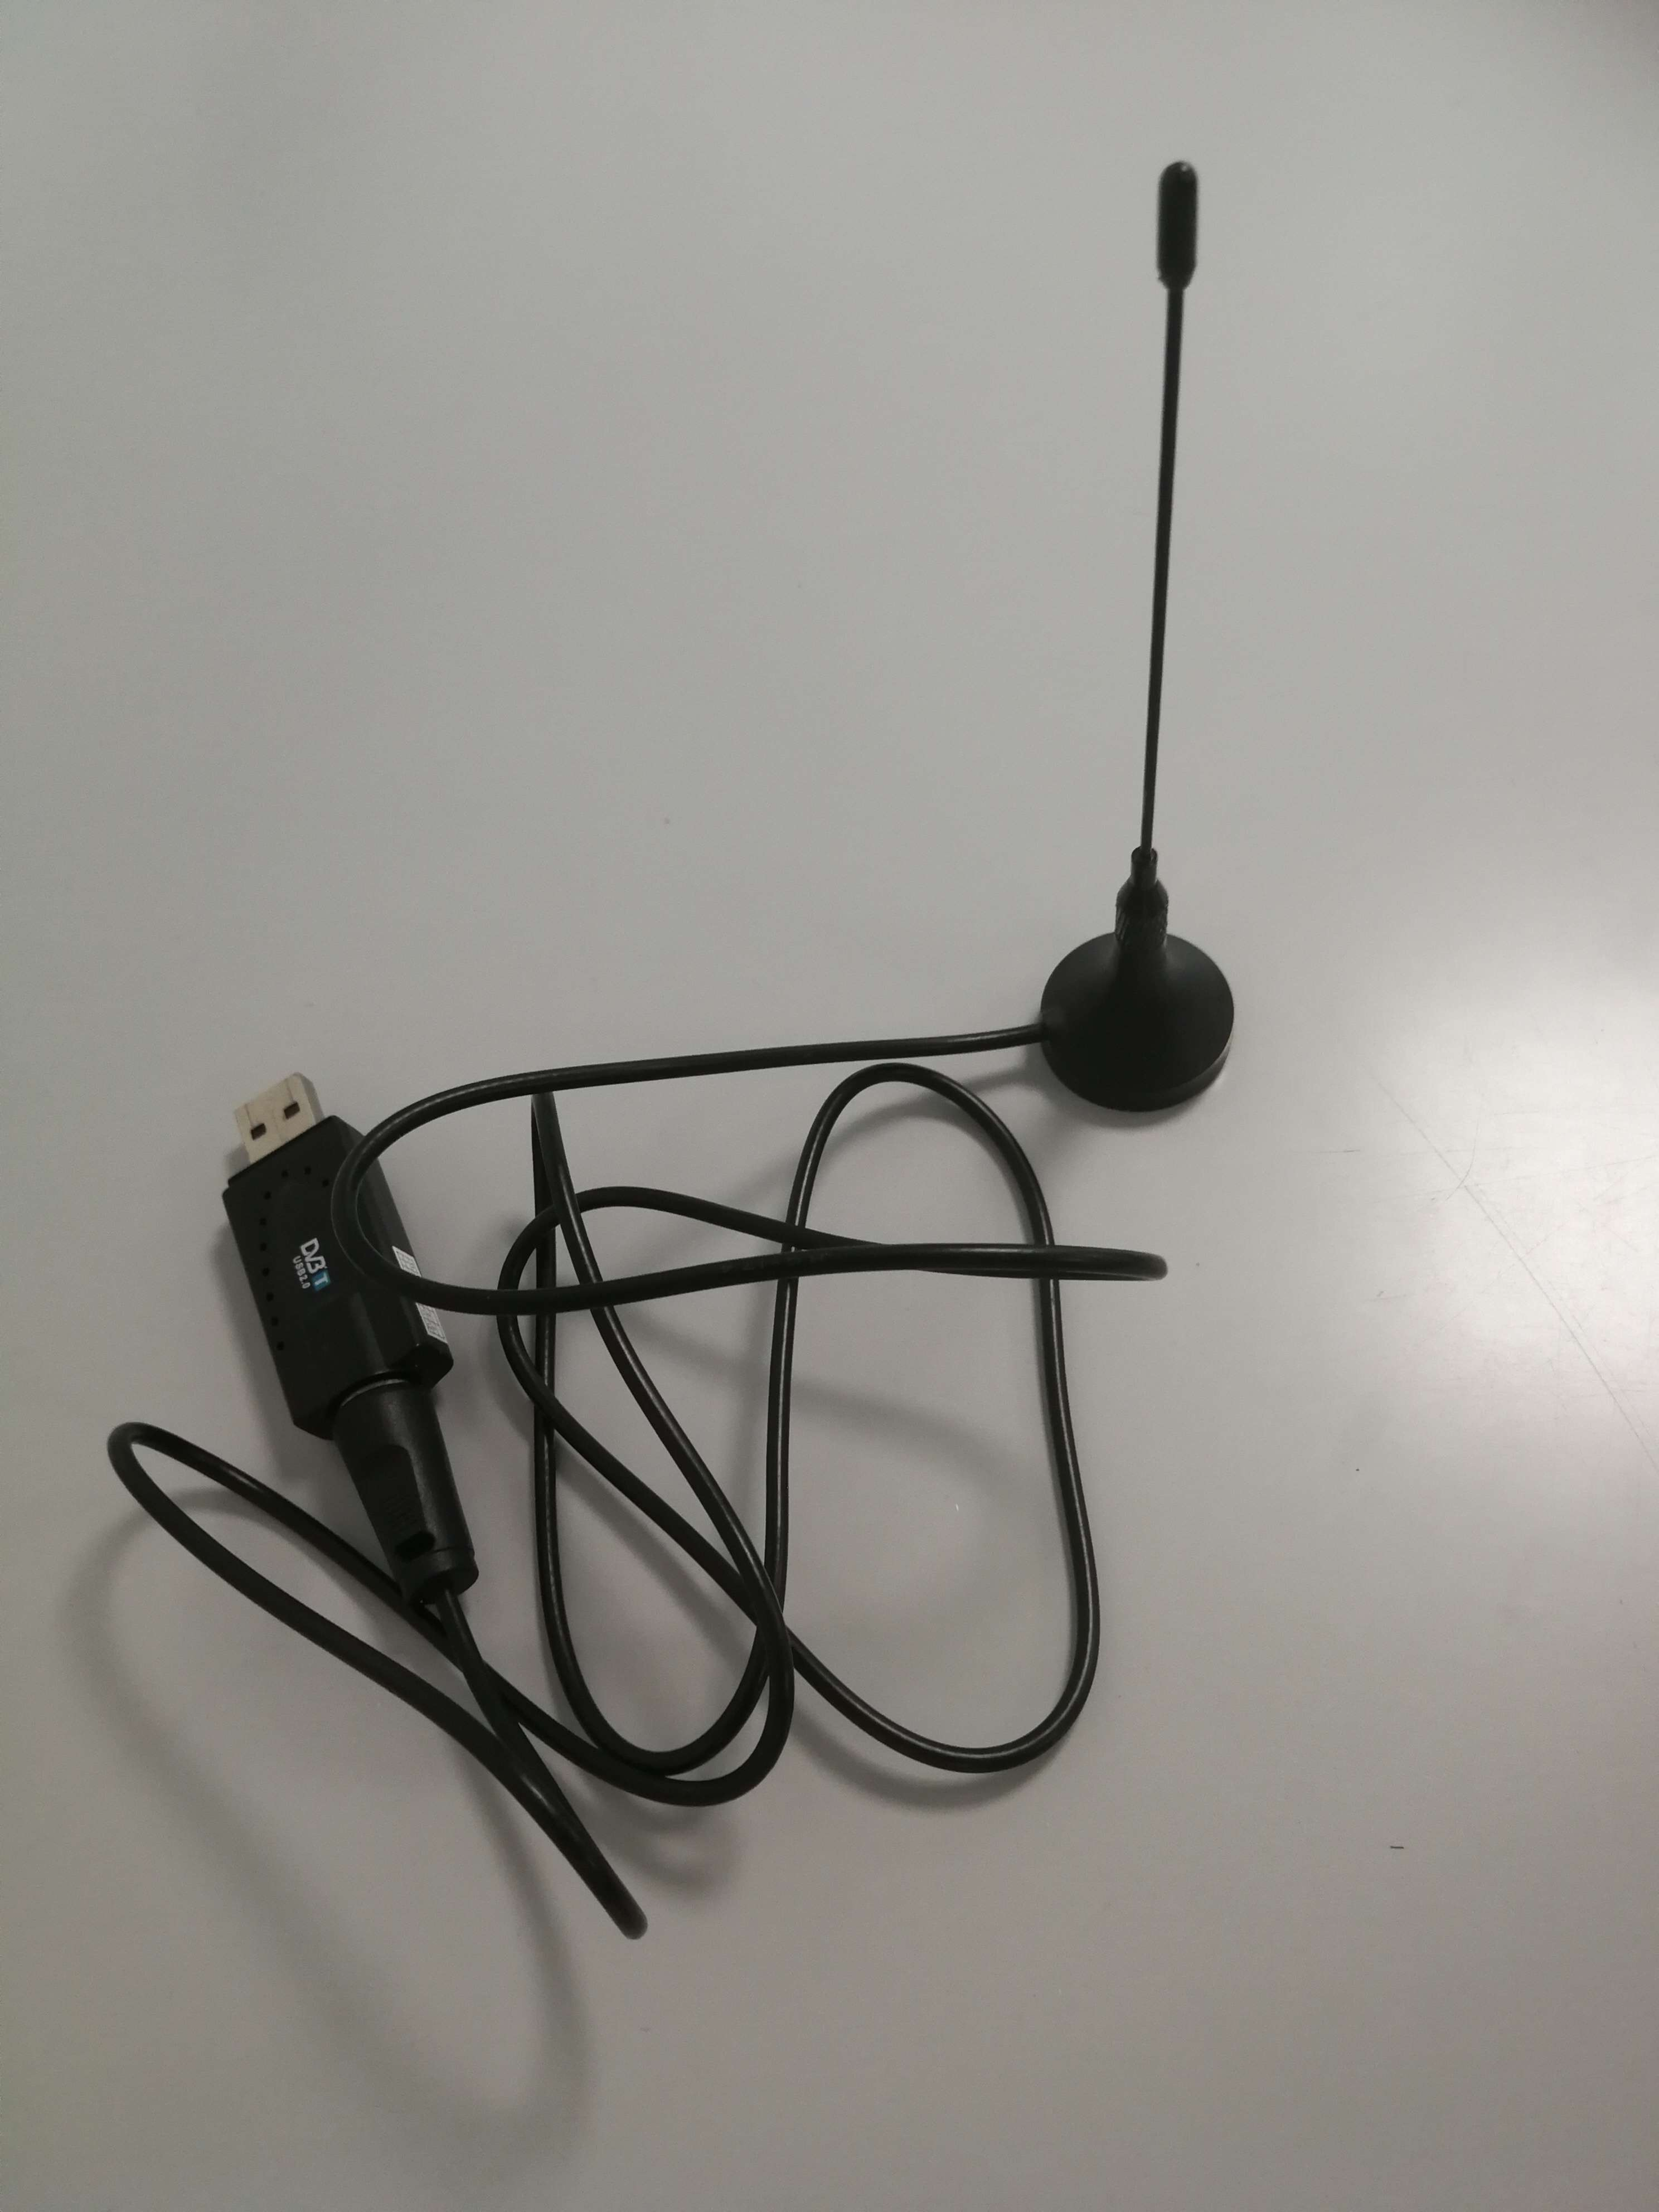
\includegraphics[scale=0.08]{images/dvbt.png}
\caption{RTL SDR DVB-T dongle}\label{term31}
\end{figure}

Le chipset RTL2832U digitalise les signaux RF et les envoie à l'ordinateur. Le tuner permet d'ajuster la fréquence pour couvrir une large portée.
La radio est raccordée à l'ordinateur via le port \ac{USB}. Le site RTL SDR \footnote{RTL-SDR : \href{https://www.rtl-sdr.com/about-rtl-sdr/}{https://www.rtl-sdr.com/about-rtl-sdr/}} ajoute quelques informations sur l'origine de l'utilisation de \ac{DVB-T} tuner en tant que \ac{SDR}. Le schéma bloc de la \ac{SDR} est représenté sur la figure \ref{term3000}. 

\newpage

\begin{figure}[h]
\centering

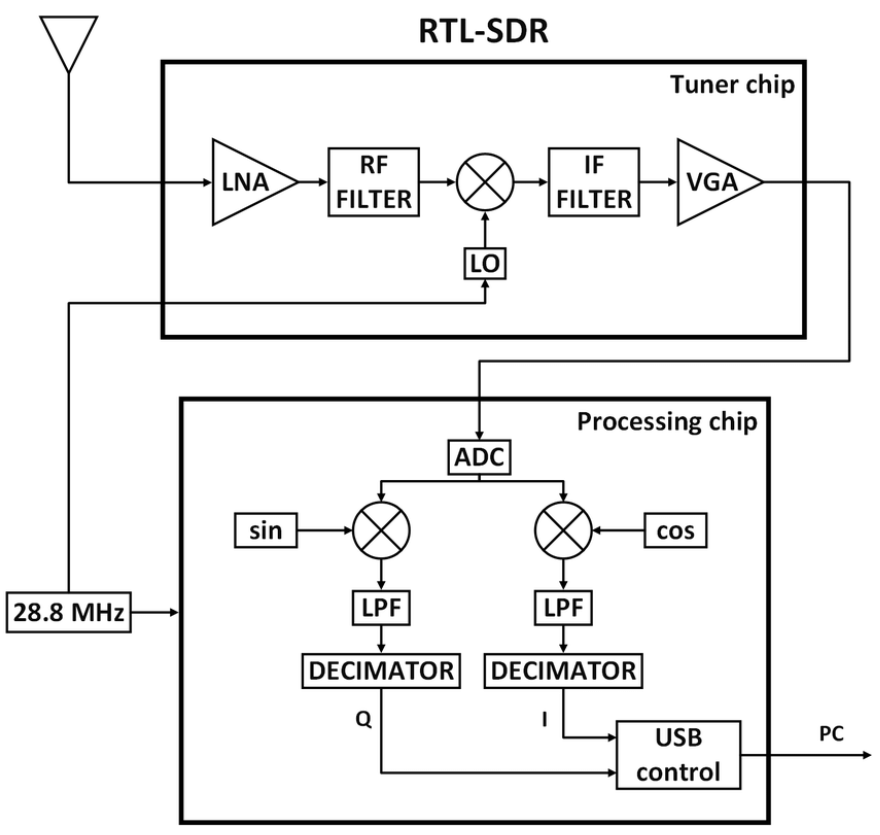
\includegraphics[scale=0.5]{images/SB-rtlsdr.png}
\caption{Schéma bloc de la RTL SDR\cite{SBrtlsdr}}\label{term3000}
\end{figure}


Le tuner comporte les éléments suivants:
\begin{itemize}
\item \textbf{\ac{LNA}}. le \ac{LNA} amplifie le signal tout en minimisant l'ajout de bruit, afin de maintenir un \ac{SNR} faible.
\item \textbf{\ac{RF} Filter}. Le filtre permettant d'isoler la fréquence désirée.
\item \textbf{\ac{LO}}. La fréquence du \ac{LO} n'est pas fixe, mais elle est contrôlée par un circuit \ac{PLL} qui utilise une horloge de référence de 28.8 MHz. Cela permet à la \ac{SDR} d'opérer sur une plage de fréquence approximative entre 24 MHz et 1.7 GHz. L'utilisation de l'oscillateur local, réglable par le \ac{PLL}, couplée au signal reçu, produit un signal à une fréquence intermédiaire.
\item \textbf{\ac{IF} Filter}. Ce filtre permet d'isoler le signal à fréquence intermédiaire. L'utilisation d'une fréquence intermédiaire est importante pour pouvoir opérer sur le signal. Par exemple, la démodu\-lation est bien plus abordable sur un signal possédant une fréquence réduite que sa valeur originale.
\item \textbf{\ac{VGA}}. Le \ac{VGA} ajuste l'amplitude du signal pour maintenir un niveau constant.
\end{itemize}

\vspace{0.1cm}

Le chipset contient les éléments suivants :
\begin{itemize}
\item \textbf{\ac{ADC}} Le signal sortant du tuner est échantillonné par l'ADC à une fréquence d'échantillonnage de 28.8MHz. L'\ac{ADC} permet de convertir un signal analogique en signal numérique.
\item \textbf{\ac{DDC}} Le signal est ramené en bande de base grâce au DDC. Le Digital Down Converter mixe le signal avec une sinusoïde complexe et applique ensuite un filtre \ac{LPF}. 
\item \textbf{Decimator}. La dernière étape utilise la décimation pour réduire le taux d'échantillonnage du signal.
\item \textbf{\ac{USB}} control. Le signal est réduit uniquement aux échantillons complexes \ac{I/Q}. Ils sont récupérés depuis l'\ac{USB} de la \ac{SDR}.
\end{itemize}

\vspace{0.1cm}

Une description détaillée du déroulement de la récupération du signal par la \ac{SDR} est disponible sur le site \textit{Ajoo's blog}\footnote{Ajoo's blog : \href{https://ajoo-github-blog-old.pages.dev/intro-to-rtl-sdr-part-i-principles-and-hardware}{https://ajoo-github-blog-old.pages
.dev/intro-to-rtl-sdr-part-i-principles-and-hardware}}.




\subsubsection{RTL-SDR R820T2}

\begin{figure}[h]
\centering

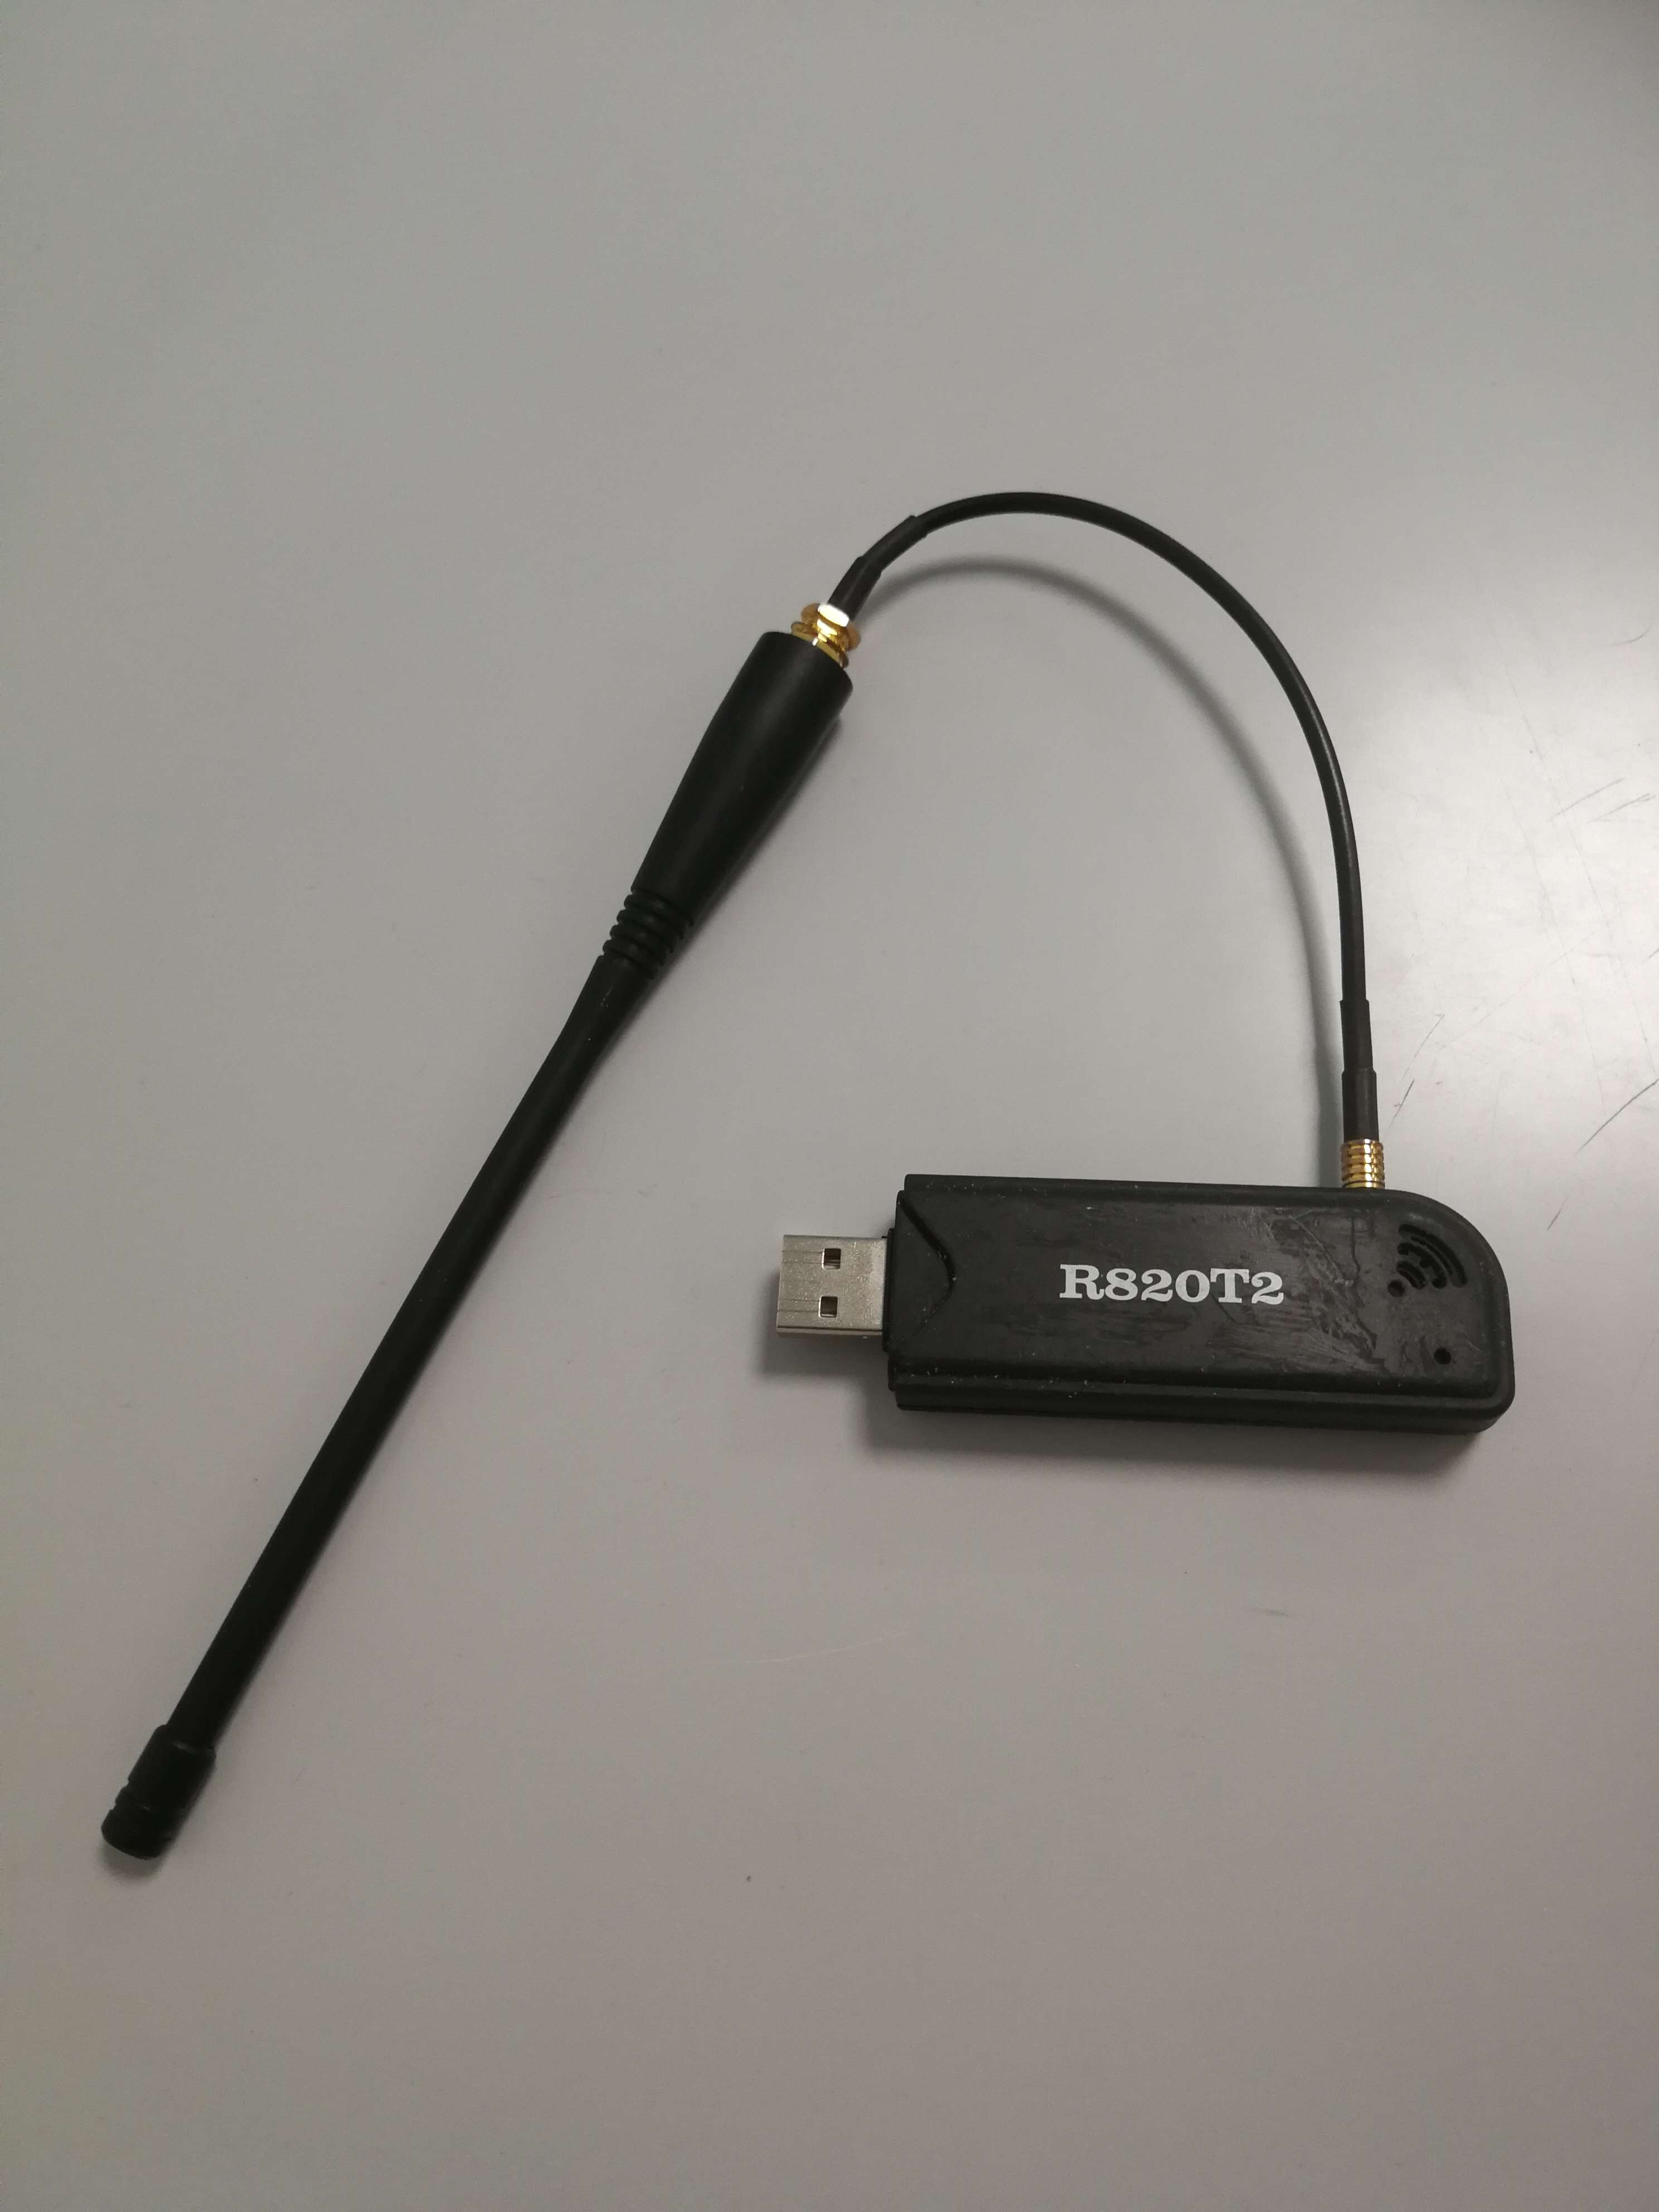
\includegraphics[scale=0.08]{images/r820t2.png}
\caption{RTL SDR R820T2}\label{term32}
\end{figure}

La deuxième radio logicielle utilisée est la \textit{RTL SDR R820T2}. Il y a deux différences majeures avec la radio \ac{DVB-T}. L'antenne de cette radio logicielle est de meilleure qualité et le tuner chip de cette \ac{SDR} est un R820T2. Cette version est une version améliorée du tuner qui se trouve dans la \ac{DVB-T}, ce qui a pour impact une réduction du bruit, une meilleure sensibilité et une couverture de fréquence plus large. La figure \ref{term32} montre la \ac{SDR} en question. Le schéma bloc de la \ac{SDR} présentée à la section \ref{dvbt} est le même que pour celui-ci. En effet la différence entre le tuner T et T2 n'est pas visible sur la description du schéma. Une description détaillée de la RTL-SDR R820T2 est disponible sur le site RTL-SDR \footnote{Datasheet R820T2 : \href{https://www.rtl-sdr.com/wp-content/uploads/2013/04/R820T_datasheet-Non_R-20111130_unlocked1.pdf}{https://www.rtl-sdr.com/wp-content/uploads/2013/04/R820T-datasheet-Non-R-20111130-unlocked1.pdf}}


\subsubsection{HackRF One}

La dernière radio logicielle utilisée est la \textit{HackRF One}. Au-delà du prix plus élevé, cette dernière radio est différente des deux autres. Elle est notamment capable de gérer la transmission et la réception de signaux, les deux autres sont uniquement des récepteurs. Si la R820T2 offrait déjà une qualité de signal supérieure à la \ac{DVB-T}, celui de la HackRF est encore plus net. La figure \ref{bothimages} montre la \ac{SDR} avec l'antenne utilisée montée sur un trépied.

\begin{figure}[h]
\centering
\begin{subfigure}{0.4\textwidth}
  \centering
  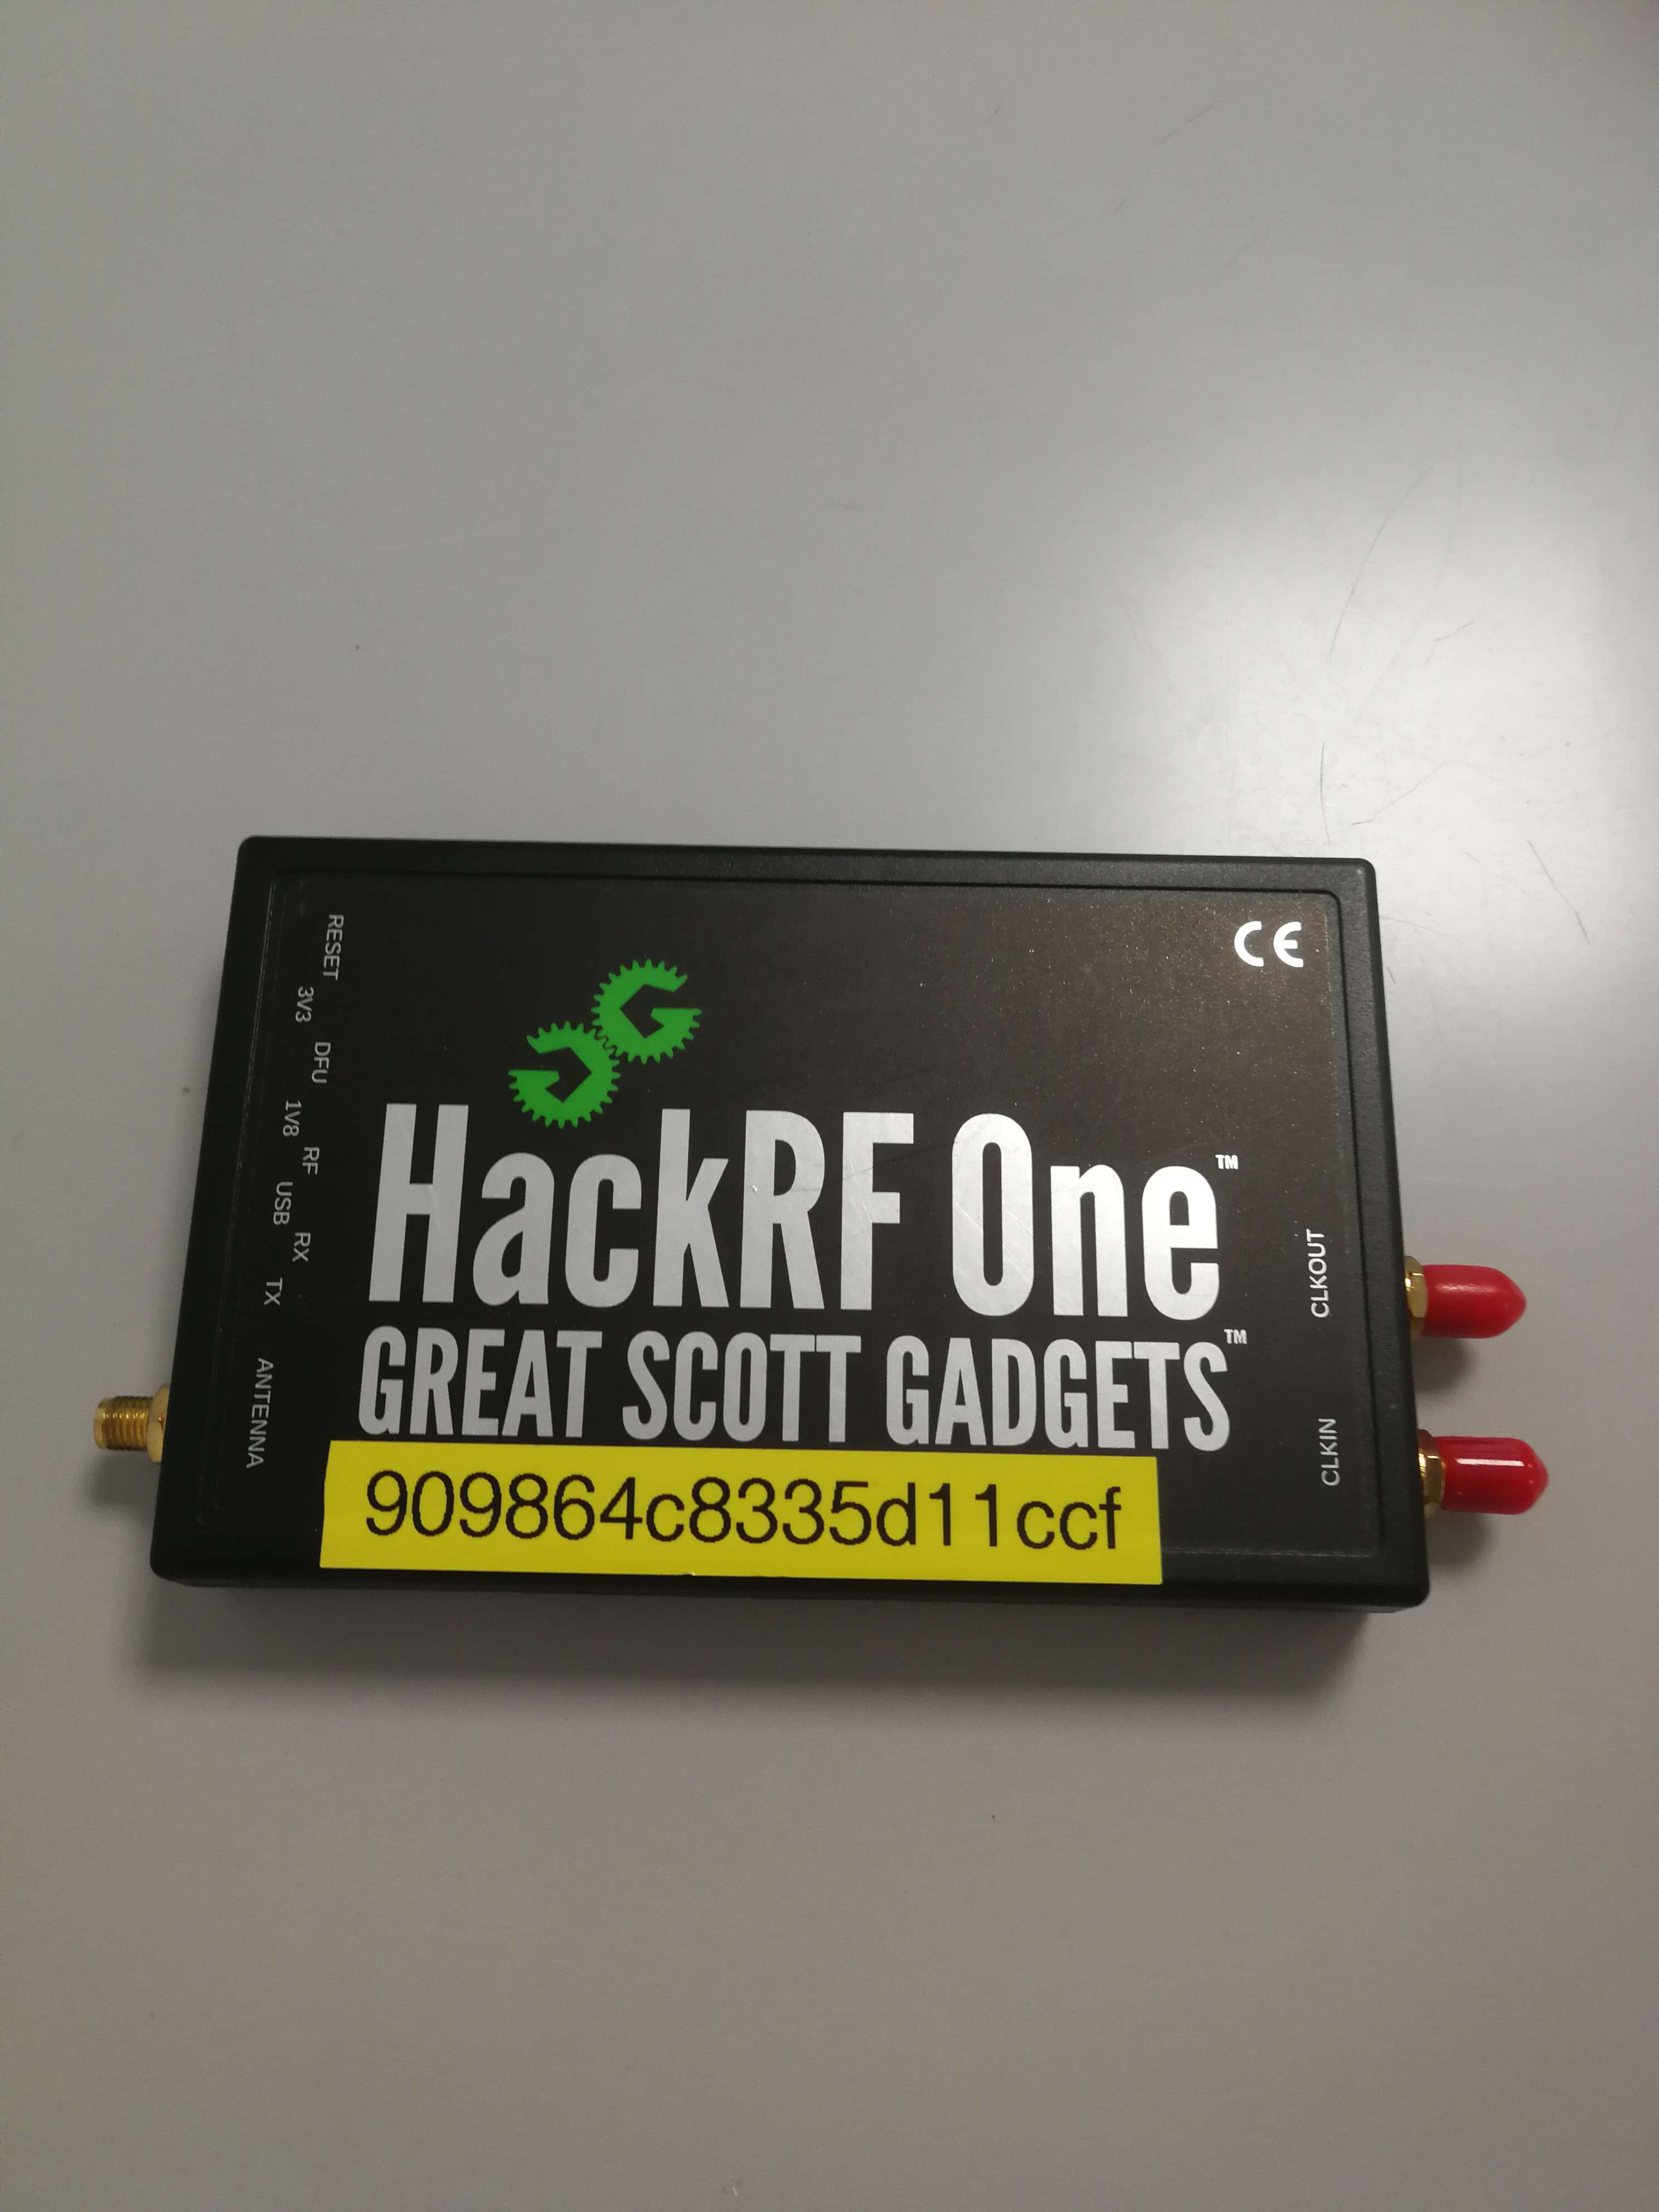
\includegraphics[width=\textwidth]{images/hackrf.png}
  \caption{SDR HackRF One}
  \label{term330}
\end{subfigure}
\hspace{0.5cm} % Adjust the horizontal space between the subfigures
\begin{subfigure}{0.4\textwidth}
  \centering
  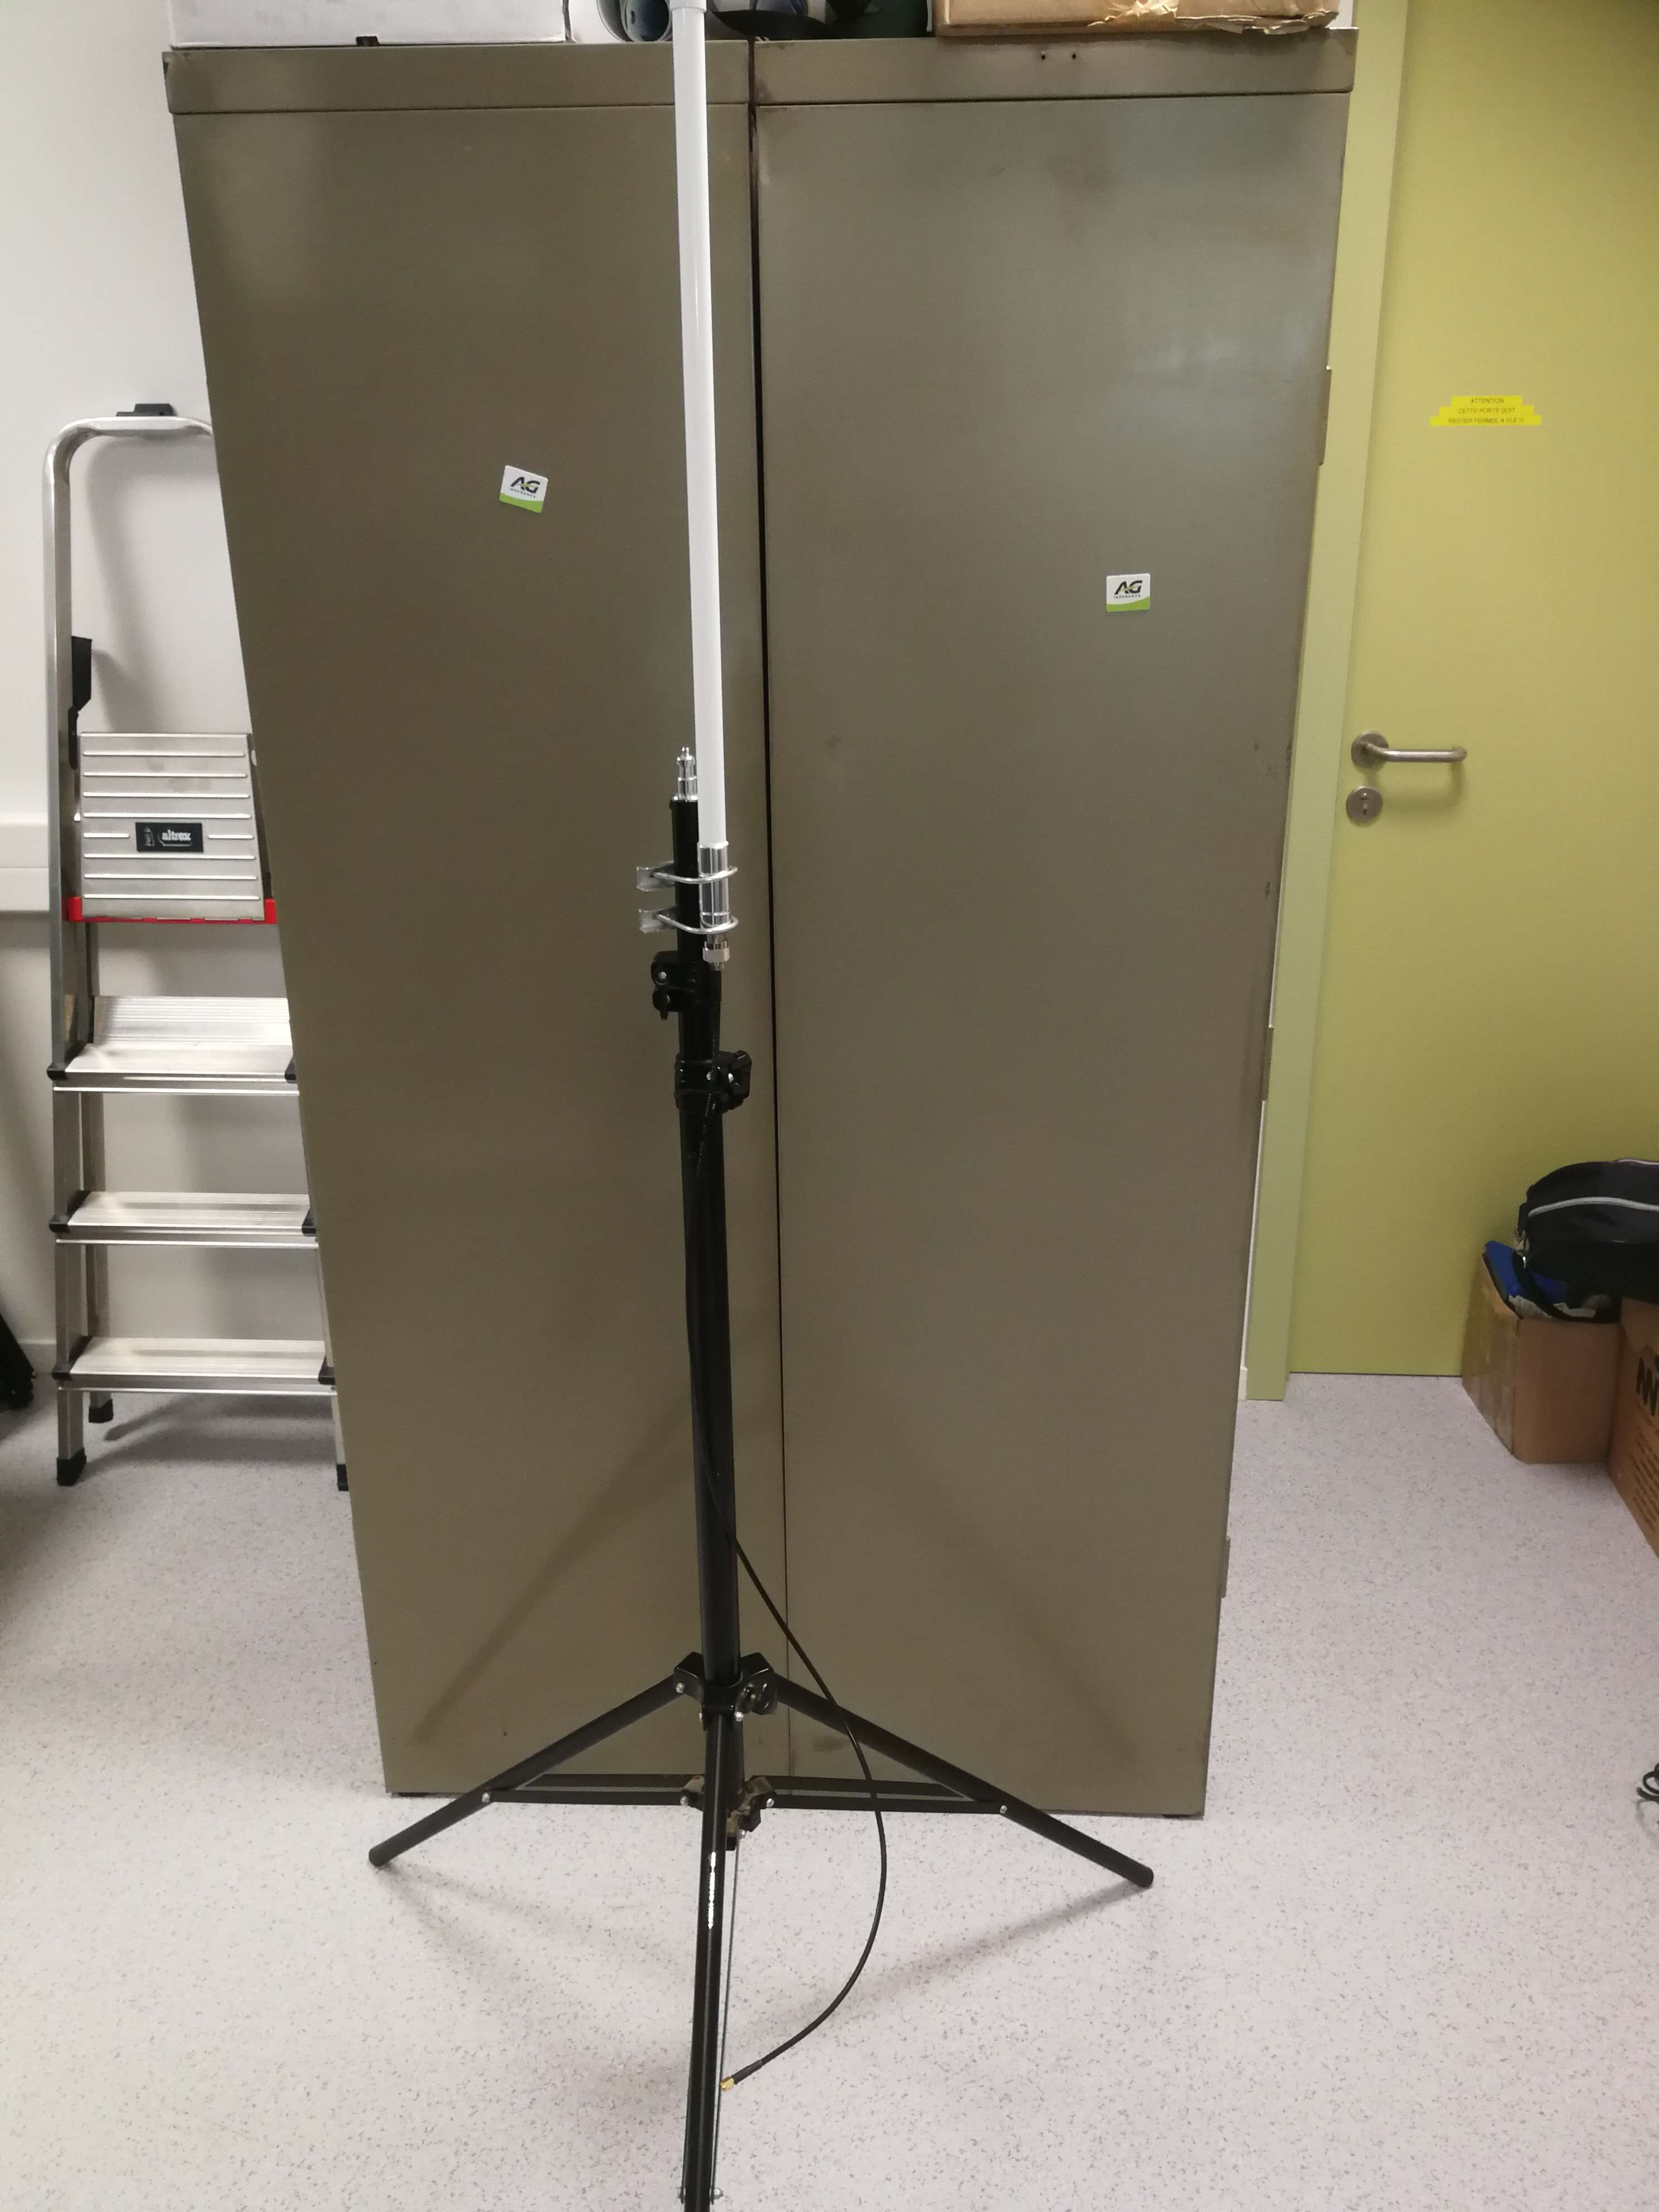
\includegraphics[width=\textwidth]{images/pied.png}
  \caption{Antenne}
  \label{term340}
\end{subfigure}
\caption{SDR HackRf One avec son antenne}
\label{bothimages}
\end{figure}


Le schéma bloc de la \ac{SDR} est affiché sur la figure \ref{term3001}. Ce dernier est beaucoup plus complexe que celui de la RTL-SDR. La HackRF est un transceiver (transmitter and receiver), donc elle possède les étapes nécessaires à l'émission que la RTL-SDR ne possède pas. Ensuite, il y a plusieurs étapes de fréquences intermédiaires. L'architecture de la HackRF \footnotemark[10] permet d'utiliser plusieurs étapes de mixeur pour atteindre la fréquence désirée. Chaque étape possède sa fréquence intermédiaire.

\begin{figure}[h]
\centering

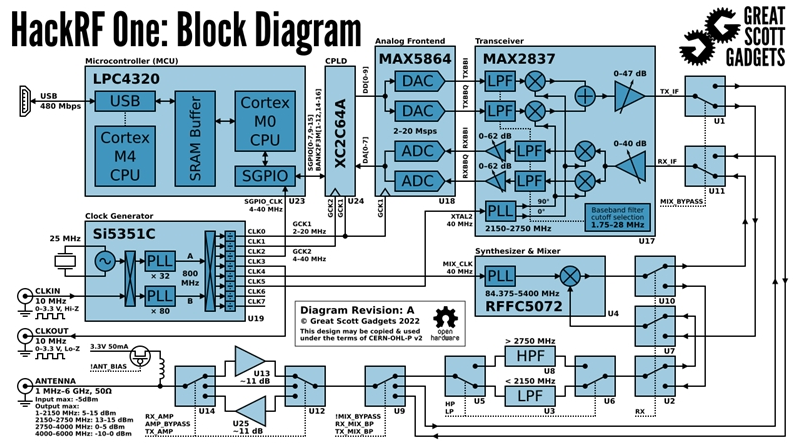
\includegraphics[scale=0.8]{images/SBhackrf.png}
\caption{Schéma bloc de la HackRF One\protect\footnotemark[10]}\label{term3001}
\end{figure}

\footnotetext[10]{HackRF One : \href{https://www.hb9afo.ch/articles/HackRF/default.htm}{https://www.hb9afo.ch/articles/HackRF/default.htm}}
 
La table \ref{table1} résume les différents critères pertinents pour les trois radios logicielles. Ces critères permettront de sélectionner la \ac{SDR} la plus adéquate pour les expérimentations.


\begin{table}[h]
\centering
\begin{adjustbox}{width=1\textwidth}
\begin{tabular}{|c|c|c|c|}
\hline
\multicolumn{1}{|c|}{} & \multicolumn{1}{c|}{RTL SDR DVB-T} & \multicolumn{1}{c|}{RTL SDR R820T2} & \multicolumn{1}{c|}{HackRF One}\\
\hline
Portée (Fréquence) & \multicolumn{2}{c|}{24MHz - 1.7GHz} & 1MHz - 6GHz \\
\hline
Taux d'échantillonnage & \multicolumn{2}{c|}{jusqu'à 3.2MHz} & jusqu'à 20MHz \\
\hline
Largeur de bande & \multicolumn{2}{c|}{jusqu'à 2.4MHz} & jusqu'à 20MHz  \\
\hline
Résolutions de l'ADC & \multicolumn{3}{c|}{8 bits} \\
\hline
RX & \multicolumn{3}{c|}{oui} \\
\hline
TX & \multicolumn{2}{c|}{non} & oui \\
\hline
Compatibilié logicielle & \multicolumn{3}{c|}{oui, notamment avec ceux décrits dans la section \ref{fft}} \\
\hline
Qualité du signal & mauvaise &\multicolumn{2}{c|}{très bonne}\\
\hline
Prix & $+-$ 20 euros & $+-$ 30 euros & $>$ 250 euros \\
\hline
\end{tabular}
\end{adjustbox}
\caption{Table comparative des radios logicielles utilisées}
\label{table1}
\end{table}



\subsection{Module d'émission Lora}

La transmission de signaux via la technologie \ac{LoRa} est un aspect essentiel du travail. Afin de garantir la meilleure qualité de transmission possible, différents modules sont testés. Cela permet de distinguer les variations de performance et de capacité entre les modules. Certains modules sont plus facilement configurables que d'autres, et d'autres nécessitent des composants hardware ou software spécifiques.

\subsubsection{Module RN2483}

\begin{figure}[h]
\centering

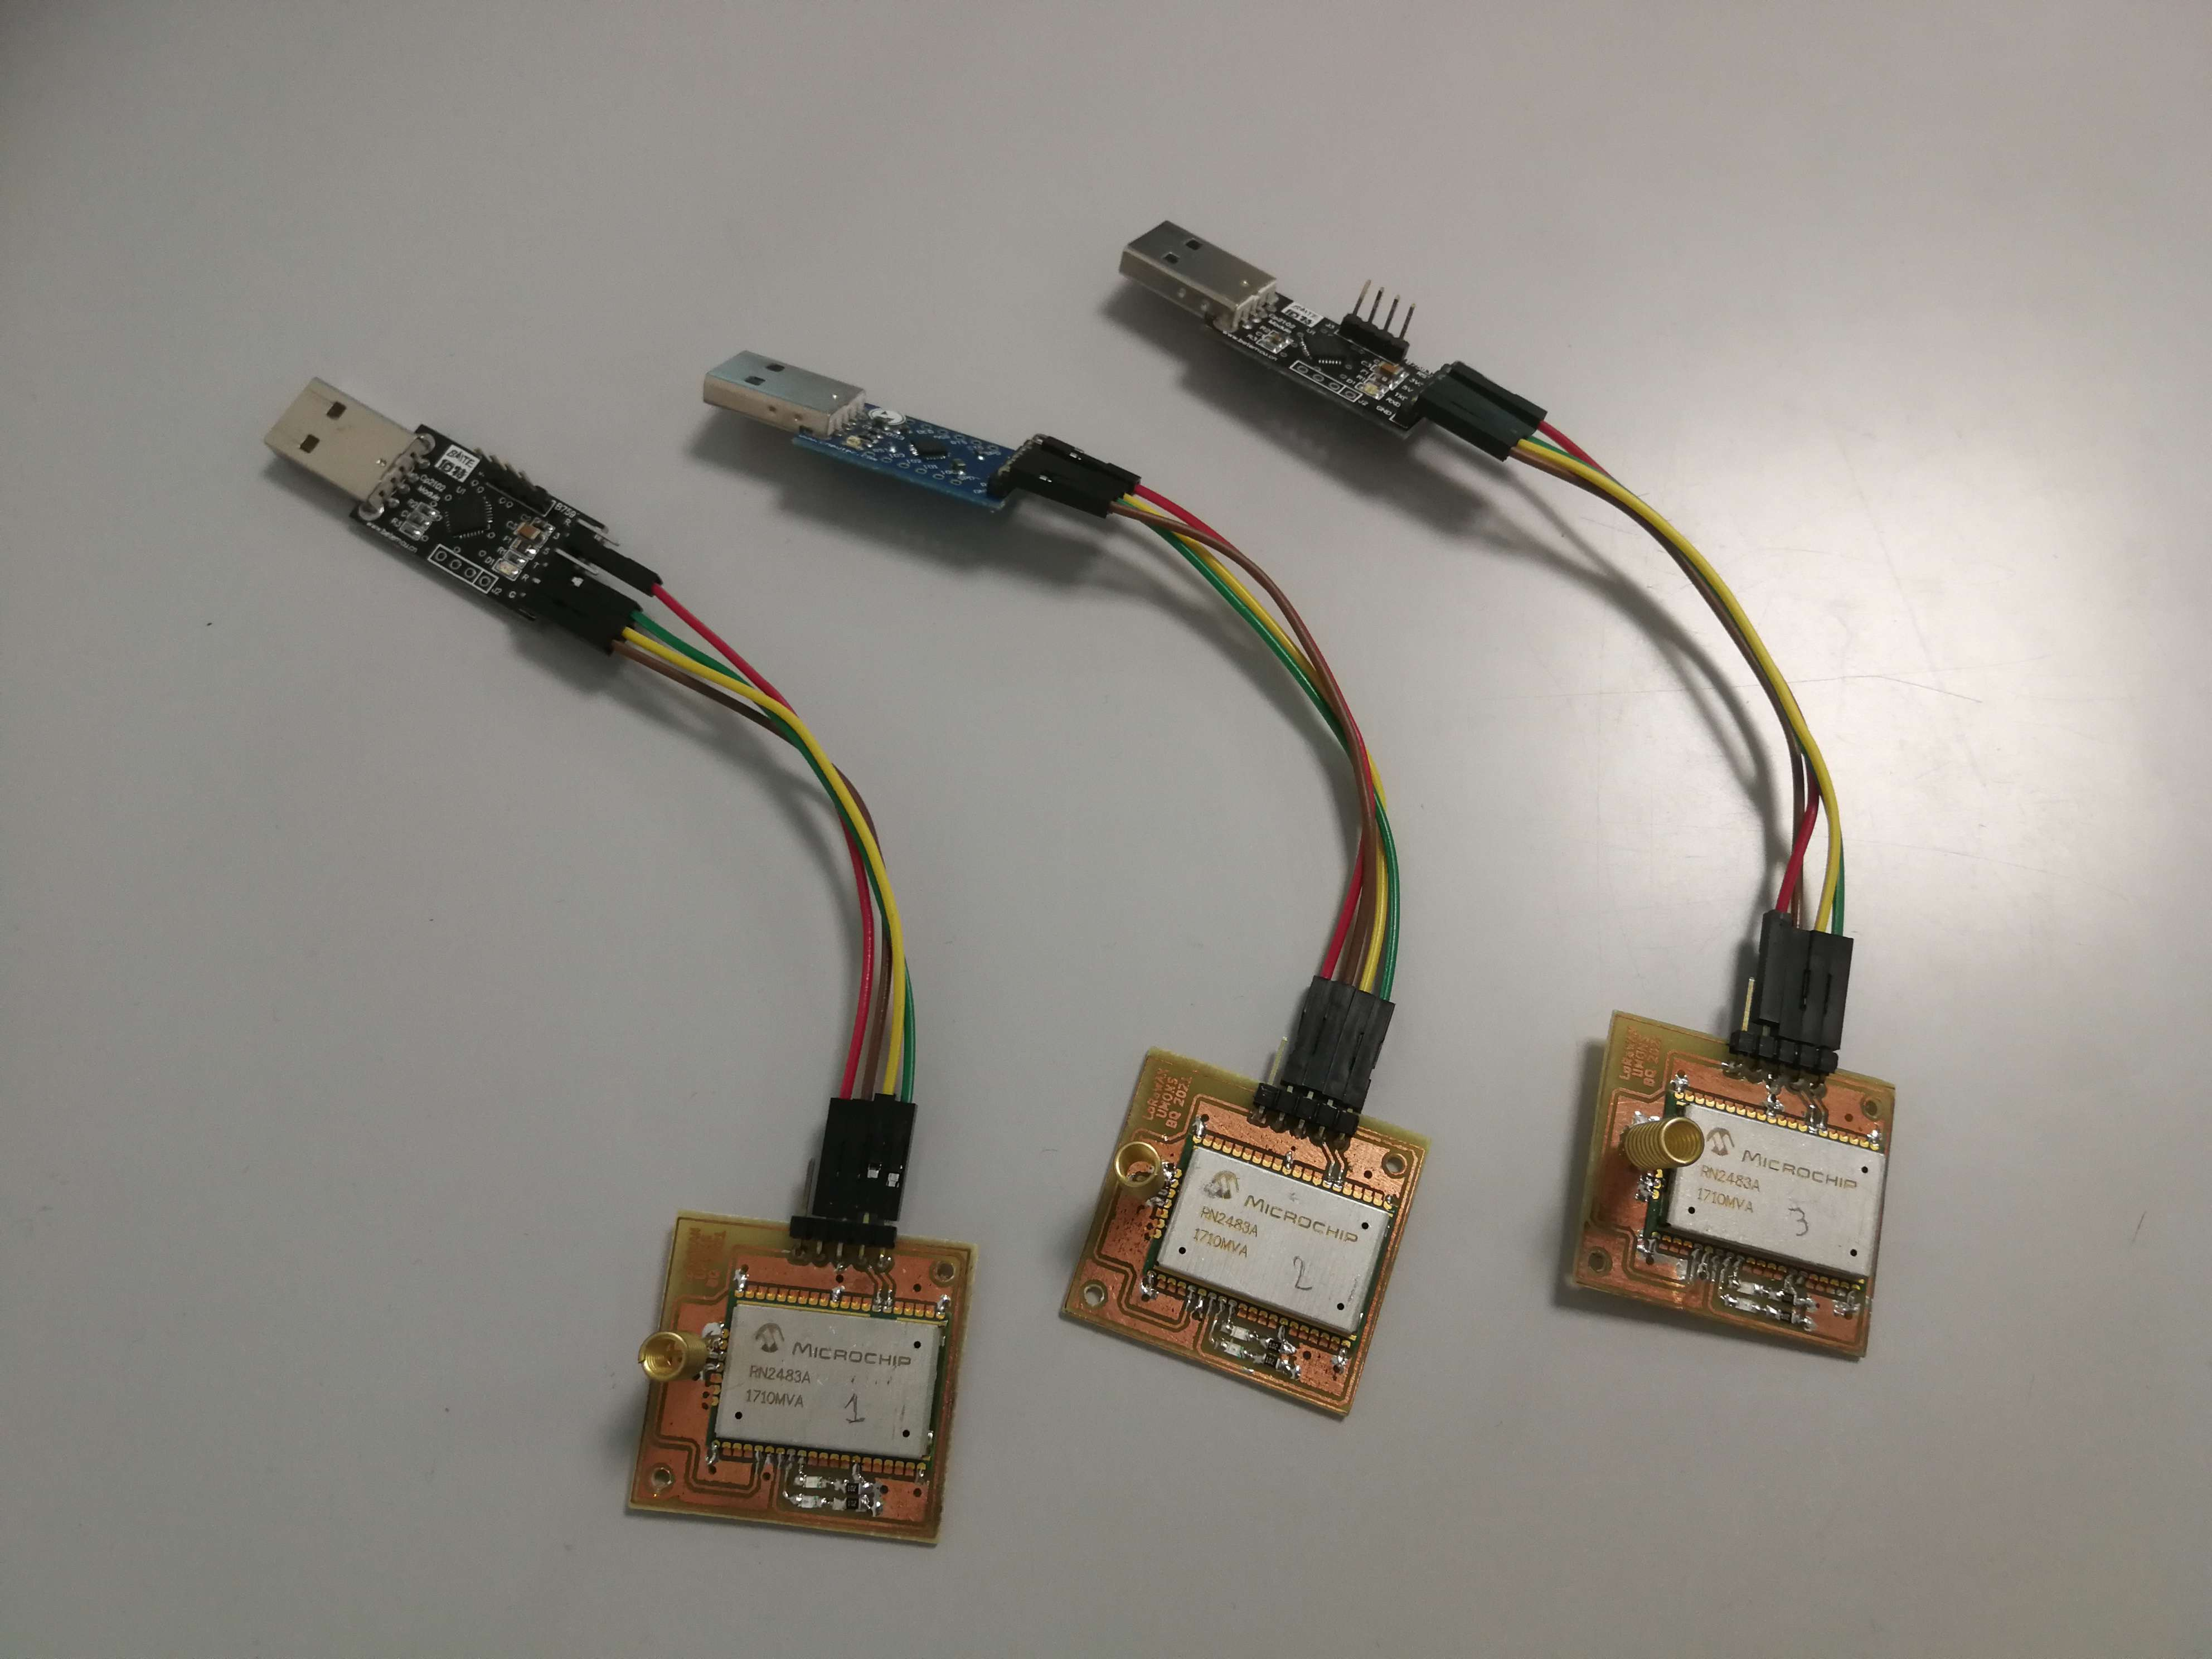
\includegraphics[scale=0.08]{images/rn2483.png}
\caption{3 modules RN2483}\label{term34}
\end{figure}


Le microchip RN2483\footnote{Datasheet RN2483 :\href{https://ww1.microchip.com/downloads/en/DeviceDoc/40001784B.pdf}{https://ww1.microchip.com/downloads
/en/DeviceDoc/}} est un module de technologie spécifique à LoRa permettant de communiquer à longue portée et à faible coût. Le Schéma bloc \footnote{Shéma bloc RN2483 : \href{https://www.mouser.be/new/microchip/microchip-rn2483-module/}{https://www.mouser.be/new/microchip/microchip-rn2483-module/}} du module est représenté à la figure \ref{term3002}. Le module RN2483 de la figure \ref{term34} est un simple transceiver radio de type SX127x couplé à un micro-contrôleur. Les informations relatives à ce type de transceivers sont disponibles sur le site de Semtech \footnote{Semtech : \href{https://www.semtech.com/products/wireless-rf/lora-connect/sx1278}{https://www.semtech.com/products/wireless-rf/lora-connect/sx1278}}.


Voici quelques spécificités du module:
\vspace{0.1cm}

\begin{itemize}
\item il comprend la technologie de modulation \ac{LoRa}, ce qui lui donne son atout de faible consommation et de longue portée. Il gère également les modulations \ac{FSK} et \ac{GFSK}.
\item Une faible consommation induit une faible puissance, le module possède un amplificateur de puissance maximale de 14dBm.
\item Les bandes de fréquences disponibles sont compatibles avec la bande \ac{ISM}. Le module couvre de 863MHz à 870MHz pour la région européenne.
\item Le data rate maximum en modulant avec LoRa est de 27343.75 bps (bits par seconde) pour un largeur de bande de 125KHz et un facteur d'étalement de 7.
\item Tous les paramètres TX sont configurables.
\end{itemize}


\begin{figure}[h]
\centering

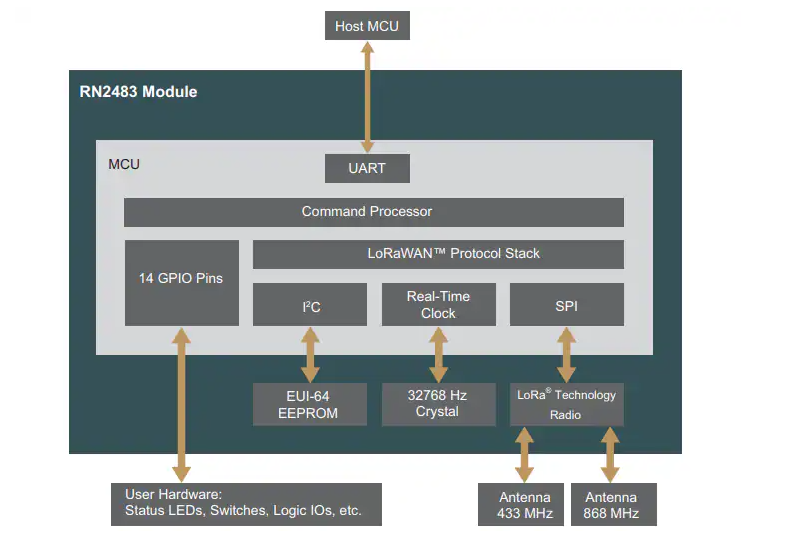
\includegraphics[scale=0.8]{images/SBrn2483.png}
\caption{Schéma bloc du module RN2483}\label{term3002}
\end{figure}

L'utilisation du module RN2483 est détaillée dans la section \ref{signallora}.

\subsubsection{Module Pycom LoPy}



Le module Pycom LoPy \footnotemark[11] est un appareil programmable en micro Python. Il comprend un micro-contrôleur ainsi qu'une série de pins digitaux input/output,  des composantes de connectivité sans fil et un port micro \ac{USB}. La figure \ref{term35} montre le module  connecté à une antenne.

\newpage

\begin{figure}[h]
\centering

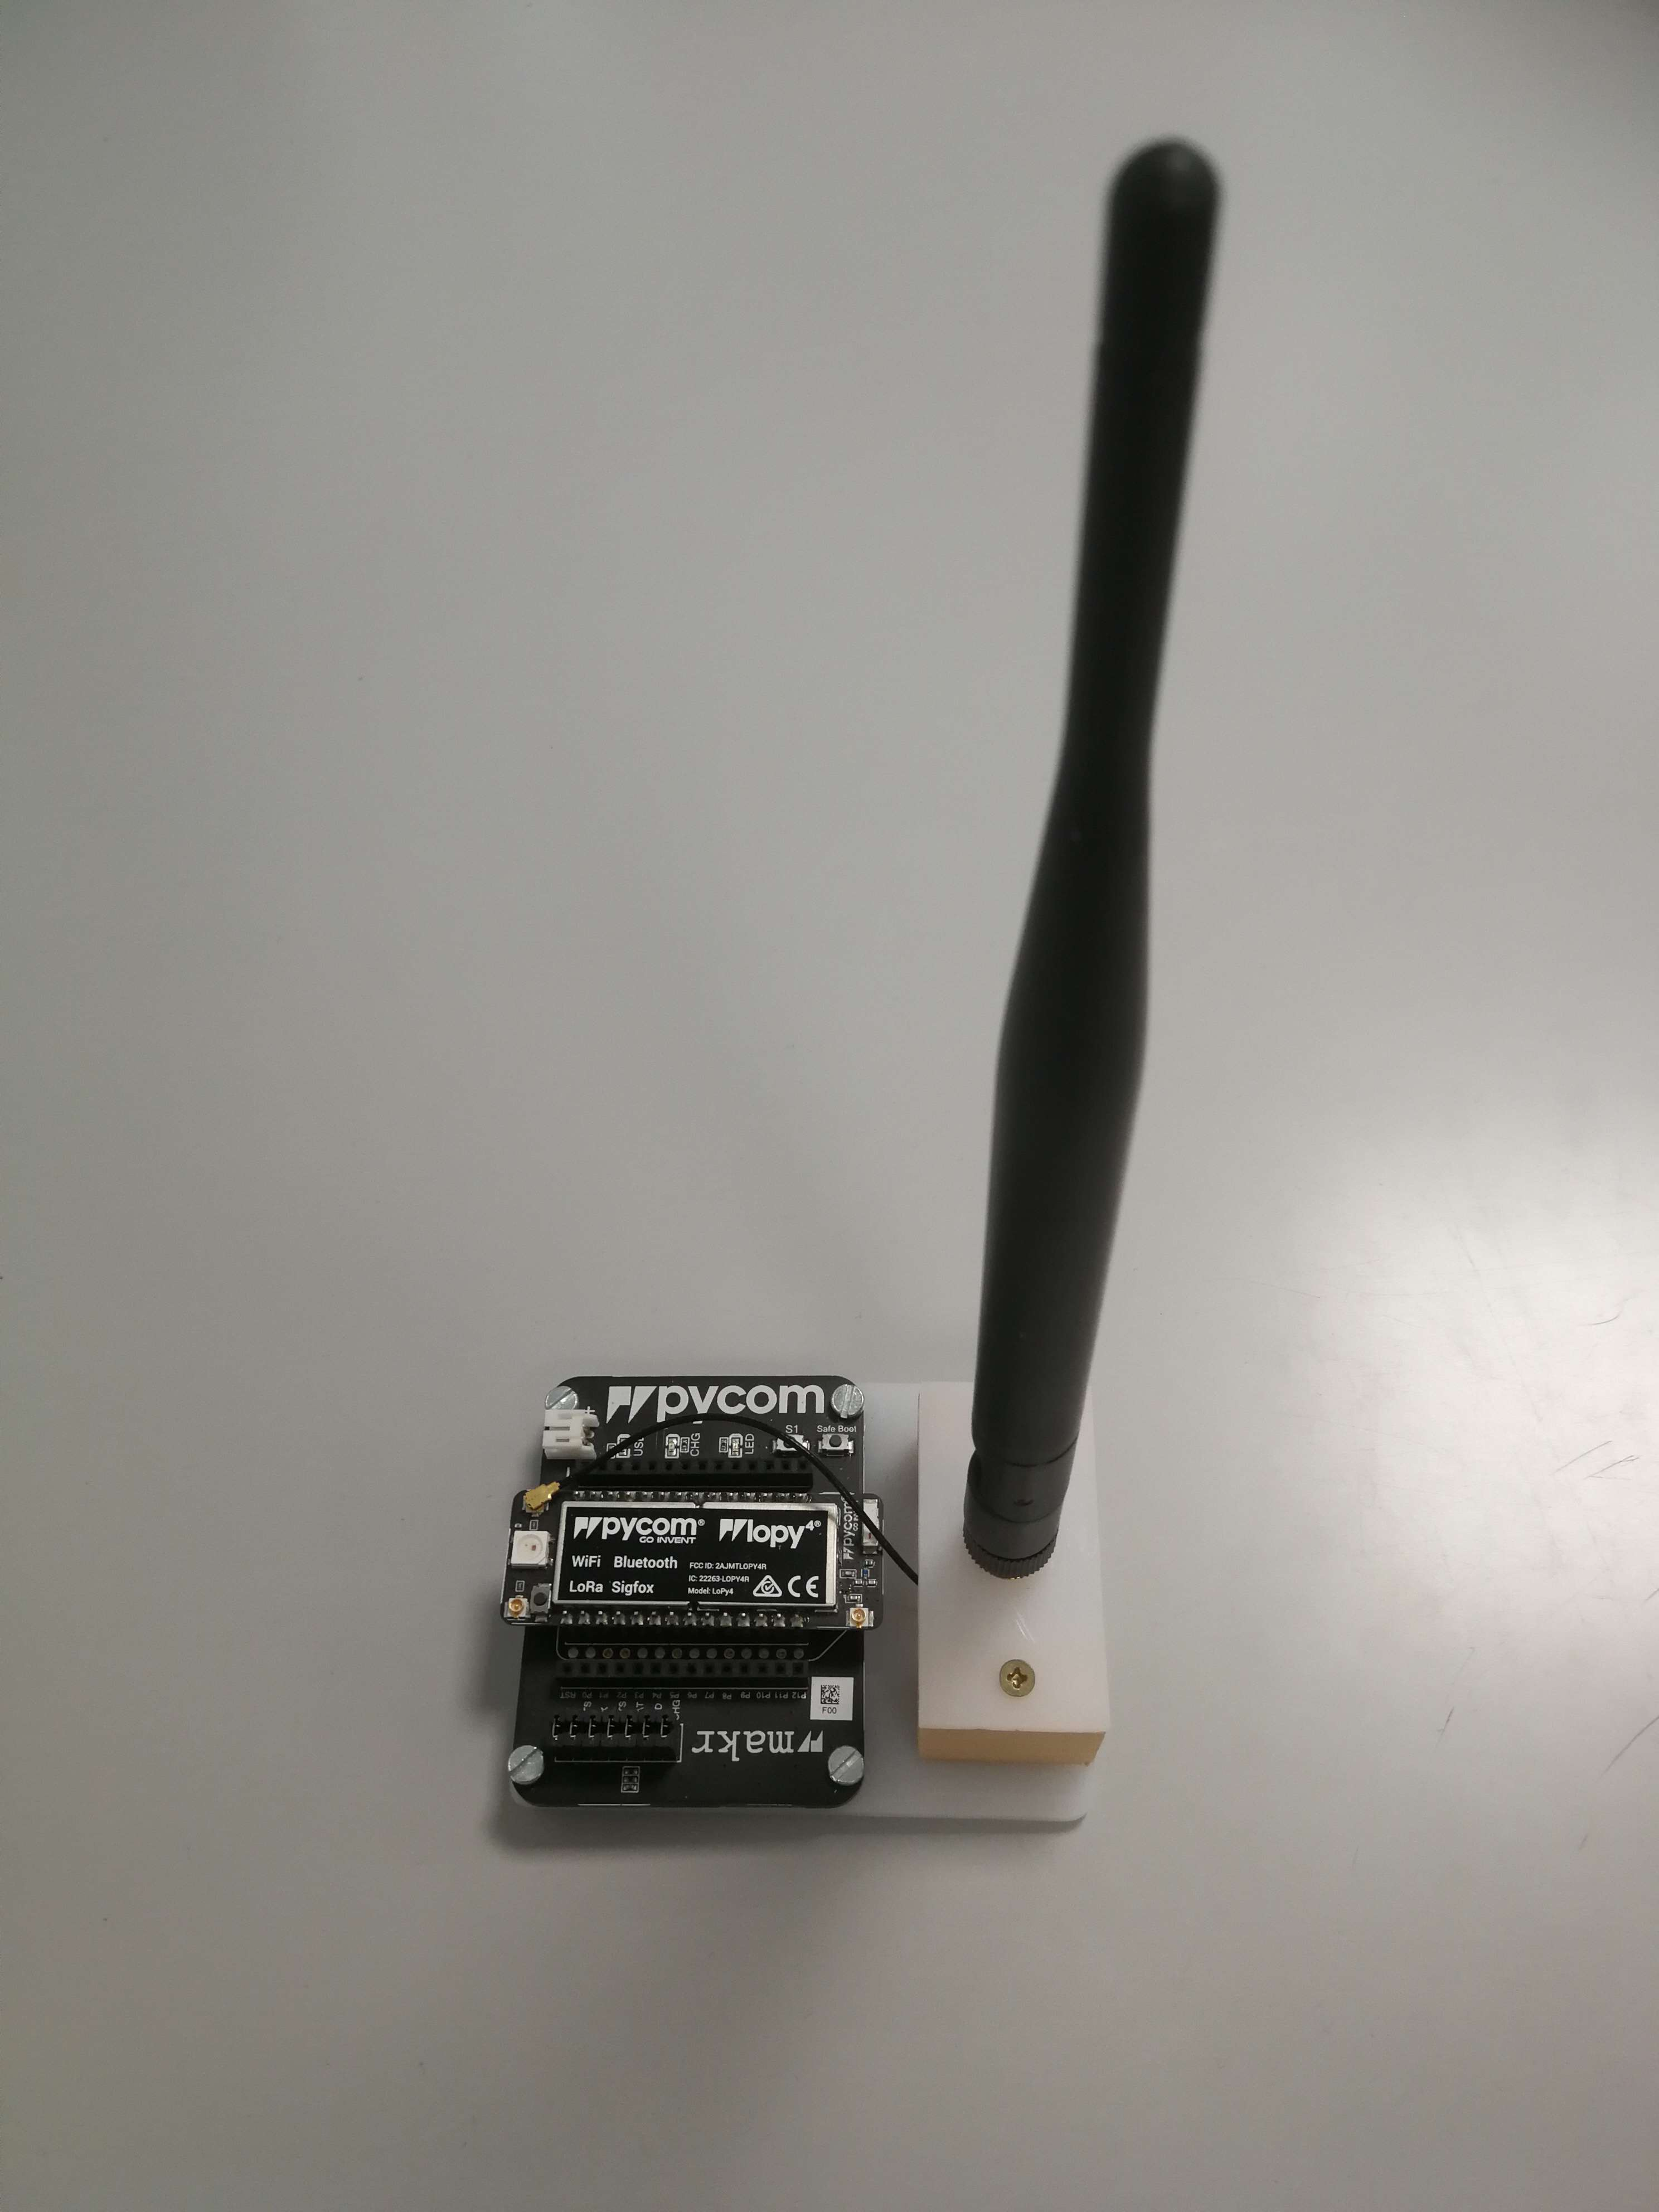
\includegraphics[scale=0.08]{images/lopy.png}
\caption{Un module Pycom lopy avec une antenne}\label{term35}
\end{figure}


Le shéma bloc \footnotemark[11]  est représenté à la figure \ref{term3003}. Contrairement au module RN2483, on remarque que le module LoPy possède des fonctions supplémentaires 
(qui ne sont pas intéressantes pour l'expérimentation) comme une connexion Wifi ou Bluetooth. Le micro-contrôleur possède aussi plusieurs interfaces autres que UART (qui est la seule disponible sur le module RN2483).

\newpage

\begin{figure}[h]
\centering

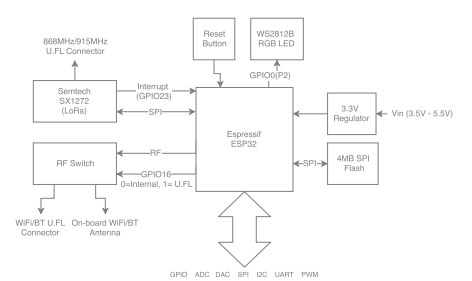
\includegraphics[scale=1]{images/SBlopy.png}
\caption{Schéma bloc du module Pycom LoPy \protect\footnotemark[11]}\label{term3003}
\end{figure}

\footnotetext[11]{Datasheet Pycom LoPy : \href{https://docs.pycom.io/gitbook/assets/specsheets/Pycom_002_Specsheets_LoPy_v2.pdf}{https://docs.pycom.io/gitbook/assets/specsheets/Pycom002SpecsheetsLoPyv2.pdf}}

\subsubsection{Module Arduino couplé à un transceiver LoRa}\label{arduino}

\begin{figure}[h]
\centering

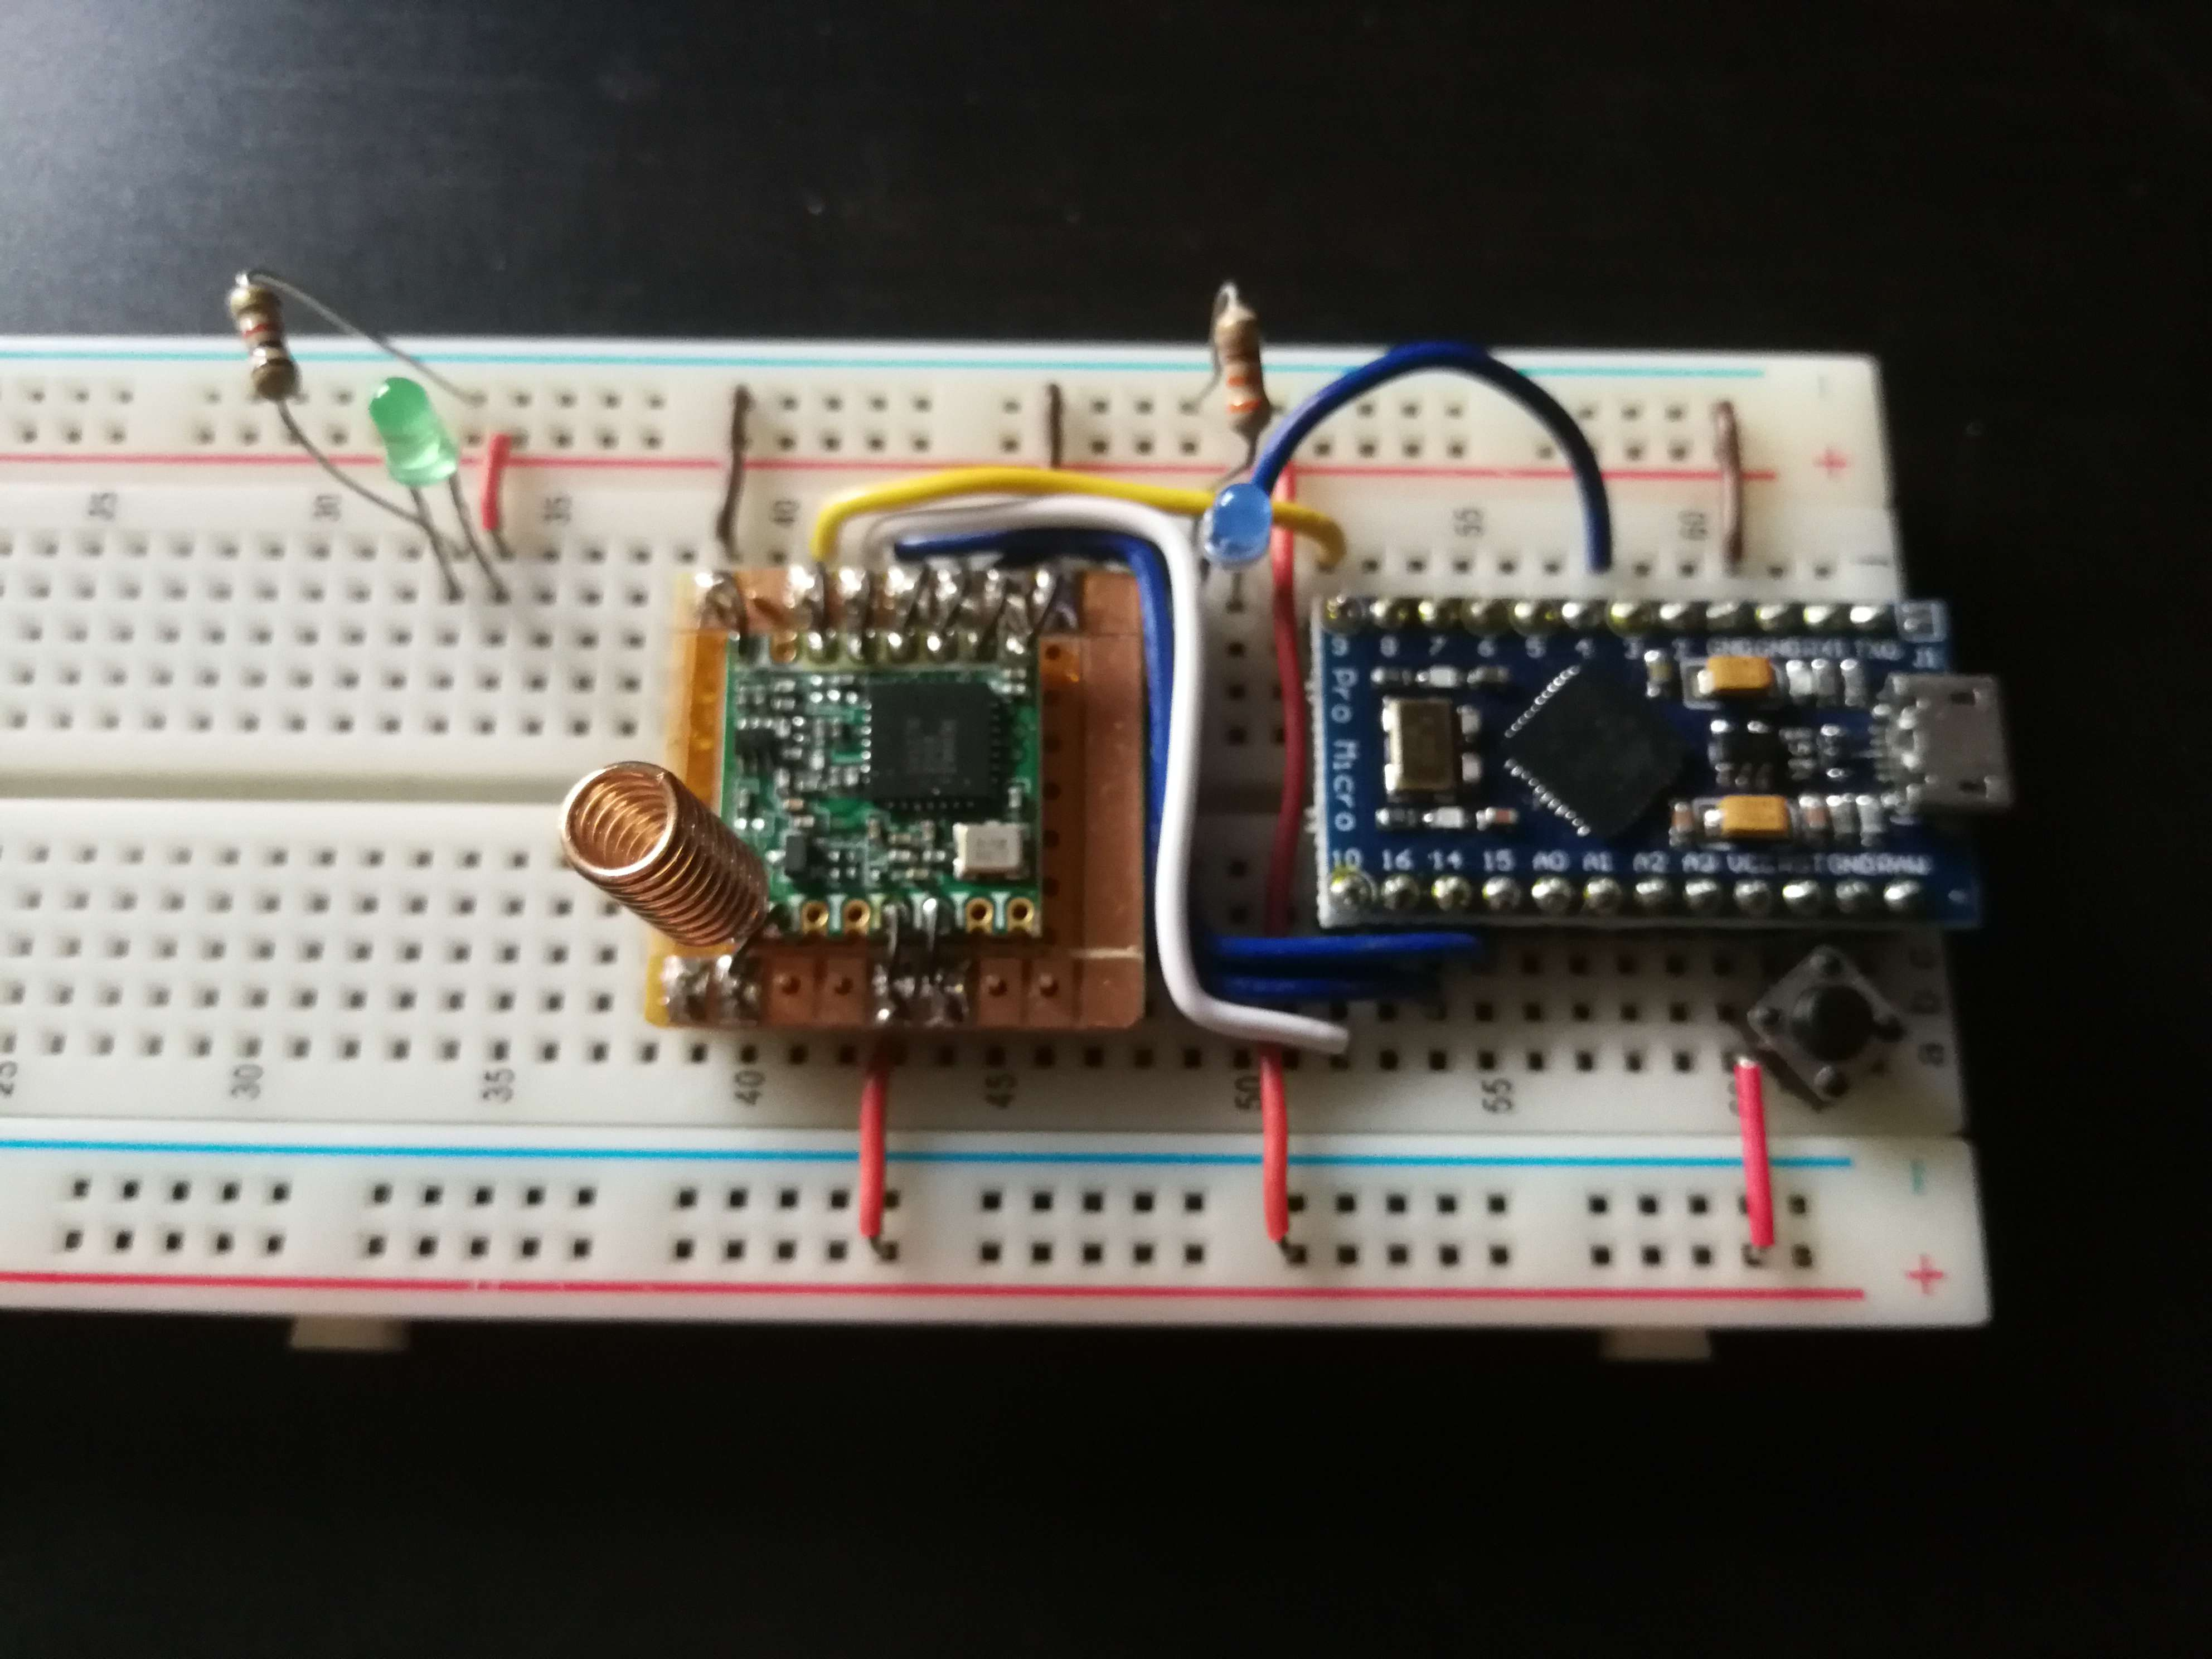
\includegraphics[scale=0.07]{images/arduino.png}
\caption{Un module Arduino}\label{term36}
\end{figure}

L'avantage principal du module Arduino \footnote{Arduino Pro Micro : \href{https://docs.arduino.cc/retired/boards/lilypad-arduino-usb/}{https://docs.arduino.cc/retired/boards/lilypad-arduino-usb/}} est qu'il est possible de configurer une largeur de bande bien plus faible qu'avec les autres modules. Les modules RN2483 ou LoPy ont une largeur de bande minimale de 125KHz, tandis qu'avec l'Arduino il est possible de descendre jusqu'à 7.8KHz. Il est également possible de réduire le facteur d'étalement en dessous de la valeur imposée par LoRa (minimum de LoRa SF = 7, ici SF = 6 possible). Pour rappel, une largeur de bande plus faible permet un \ac{TOA} plus grand, ce qui est très utile pour analyser les signaux. Le transceiver est de type SX127x (comme celui du RN2483).

\vspace{0.1cm}

L'utilisation de l'\ac{IDE} Arduino 2.2.1 est nécessaire pour la configuration du module Arduino décrit dans la section \ref{arduino}. L'\ac{IDE} permet d'uploader le code  dans le module. Le code est disponible dans l'annexe \ref{codearduino}.

\subsection{Logiciels}\label{fft}

Une fois les différents appareils choisis, il faut les accompagner avec les softwares adéquats. Ainsi il faut des logiciels d'analyse de signaux compatibles avec les différents modules et radios logicielles.

\subsubsection{GQRX}

Le premier logiciel choisi est GQRX \footnote{GQRX : \href{https://www.gqrx.dk}{https://www.gqrx.dk}}. C'est un logiciel open source d'analyse de fréquences radio pour les \ac{SDR}. La figure \ref{term37} montre comment configurer le logiciel.

\begin{figure}[h]
\centering
\begin{subfigure}{0.35\textwidth}
  \centering
  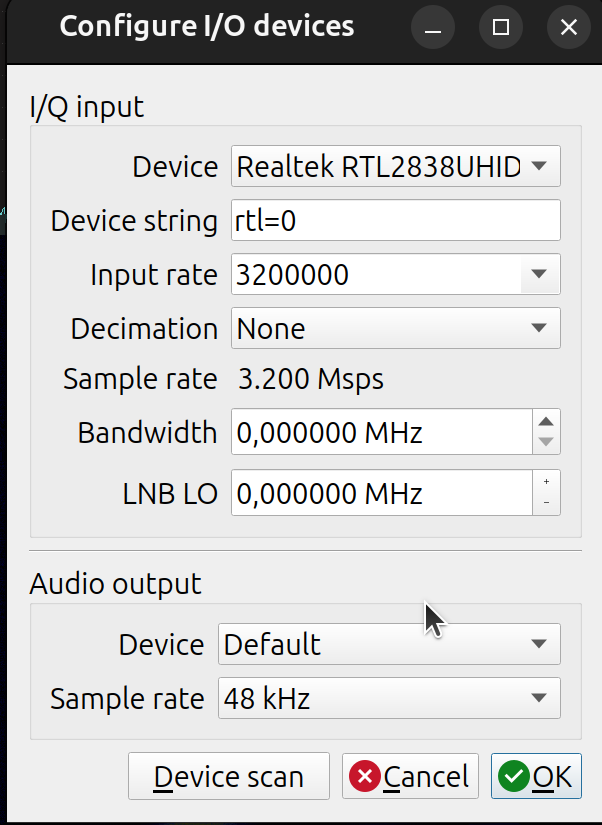
\includegraphics[width=\textwidth]{images/gqrx2.png}
  \caption{SDR input}
  \label{term331}
\end{subfigure}
\hspace{0.5cm} % Adjust the horizontal space between the subfigures
\begin{subfigure}{0.35\textwidth}
  \centering
  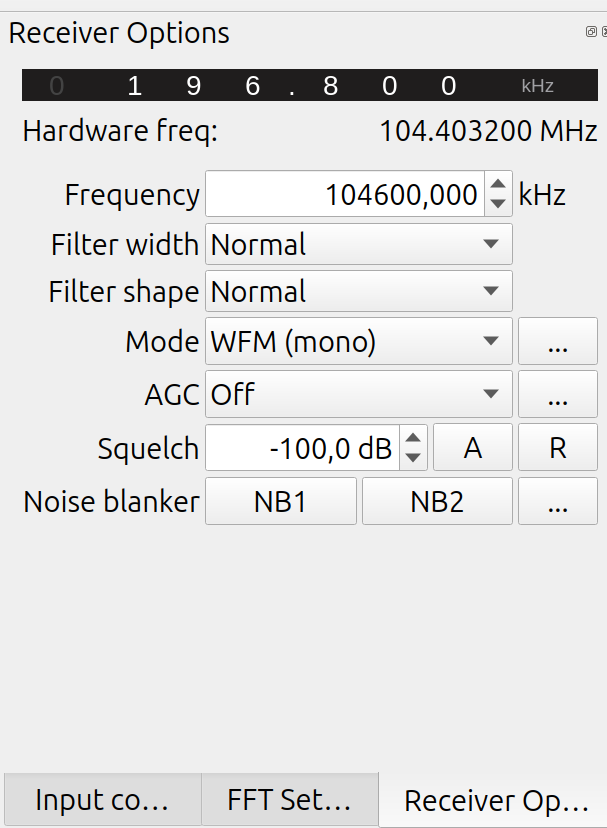
\includegraphics[width=\textwidth]{images/gqrx3.png}
  \caption{Receiver options}
  \label{term341}
\end{subfigure}
\caption{Configuration de GQRX}
\label{term37}
\end{figure}

La figure \ref{term331} demande de compléter les paramètres suivants:

\vspace{0.1cm}

\begin{itemize}
\item \textbf{Device}: il faut sélectionner la \ac{SDR} dans la liste des appareils. Le Device String fait référence à cet appareil dans GQRX.
\item \textbf{Input rate}: le taux d'échantillonnage capturé par la \ac{SDR}, il apparît plus bas comme sample rate.
\item \textbf{Decimation}: c'est un procédé qui permet de réduire le nombre d'échan\-tillons gérés par le logiciel, pour économiser des ressources.
\item \textbf{\ac{BW}}: la largeur de bande supplémentaire que peut gérer la \ac{SDR}.
\item \textbf{\ac{LNB LO}}: ce paramètre est spécifi\-que à la réception satellite et représente le frequency offset appliqué par l'oscillateur local dans un LNB downconverter.
\item L'\textbf{Audio output} concerne la sortie sonore du signal.
\end{itemize}

\vspace{0.1cm}

La figure \ref{term341} ajoute des paramètres pour le récepteur, c'est-à-dire pour l'interface de GQRX :

\vspace{0.1cm}

\begin{itemize}
\item \textbf{Frequency}: la fréquence que l'on souhaite écouter.
\item \textbf{Filter Width}: ce paramètre permet de changer la taille de la largeur de bande du filtre appliqué au signal.
\item \textbf{Filter Shape}: contrairement au Filter Width, ce n'est pas la taille mais la forme du filtre que l'on peut modifier.
\item \textbf{Mode}: le mode de démodulation.
\item \textbf{\ac{ACG}}: l'\ac{ACG} ajuste le gain du récepteur pour maintenir un signal constant.
\item \textbf{Squelch}: c'est un threshold qui coupe la sortie sonore s'il est franchi.
\item \textbf{Noise blanker}: c'est une fonctionnalité qui permet de réduire l'impact des interférences sur le signal.
\end{itemize}

\vspace{0.1cm}

La figure \ref{term38} montre un exemple de ce qu'on observe quand on écoute la fréquence radio de Classic21. GQRX affiche le signal reçu sous deux formes différentes : en spectre et en cascade.

\vspace{0.1cm}

L'affichage du spectre fournit une représentation graphique en temps réel du spectre RF sur une gamme de fréquences.
Il montre la puissance du signal de différentes fréquences sur une plage de fréquences spécifiée.
L'axe horizontal représente la fréquence, tandis que l'axe vertical affiche la force du signal (mesurée en dB).

\vspace{0.1cm}

L'affichage en cascade est un spectrogramme qui visualise la force du signal au fil du temps.
Il montre une série de spectres instantanés empilés les uns sur les autres, où l'intensité de la couleur représente la force du signal.
Chaque ligne horizontale du tracé en cascade représente une vue du spectre capturée à un moment précis, créant ainsi un enregistrement de l'activité du signal.
L'axe horizontal représente la fréquence et l'axe vertical représente le temps.

\newpage

\begin{figure}[h]
\centering

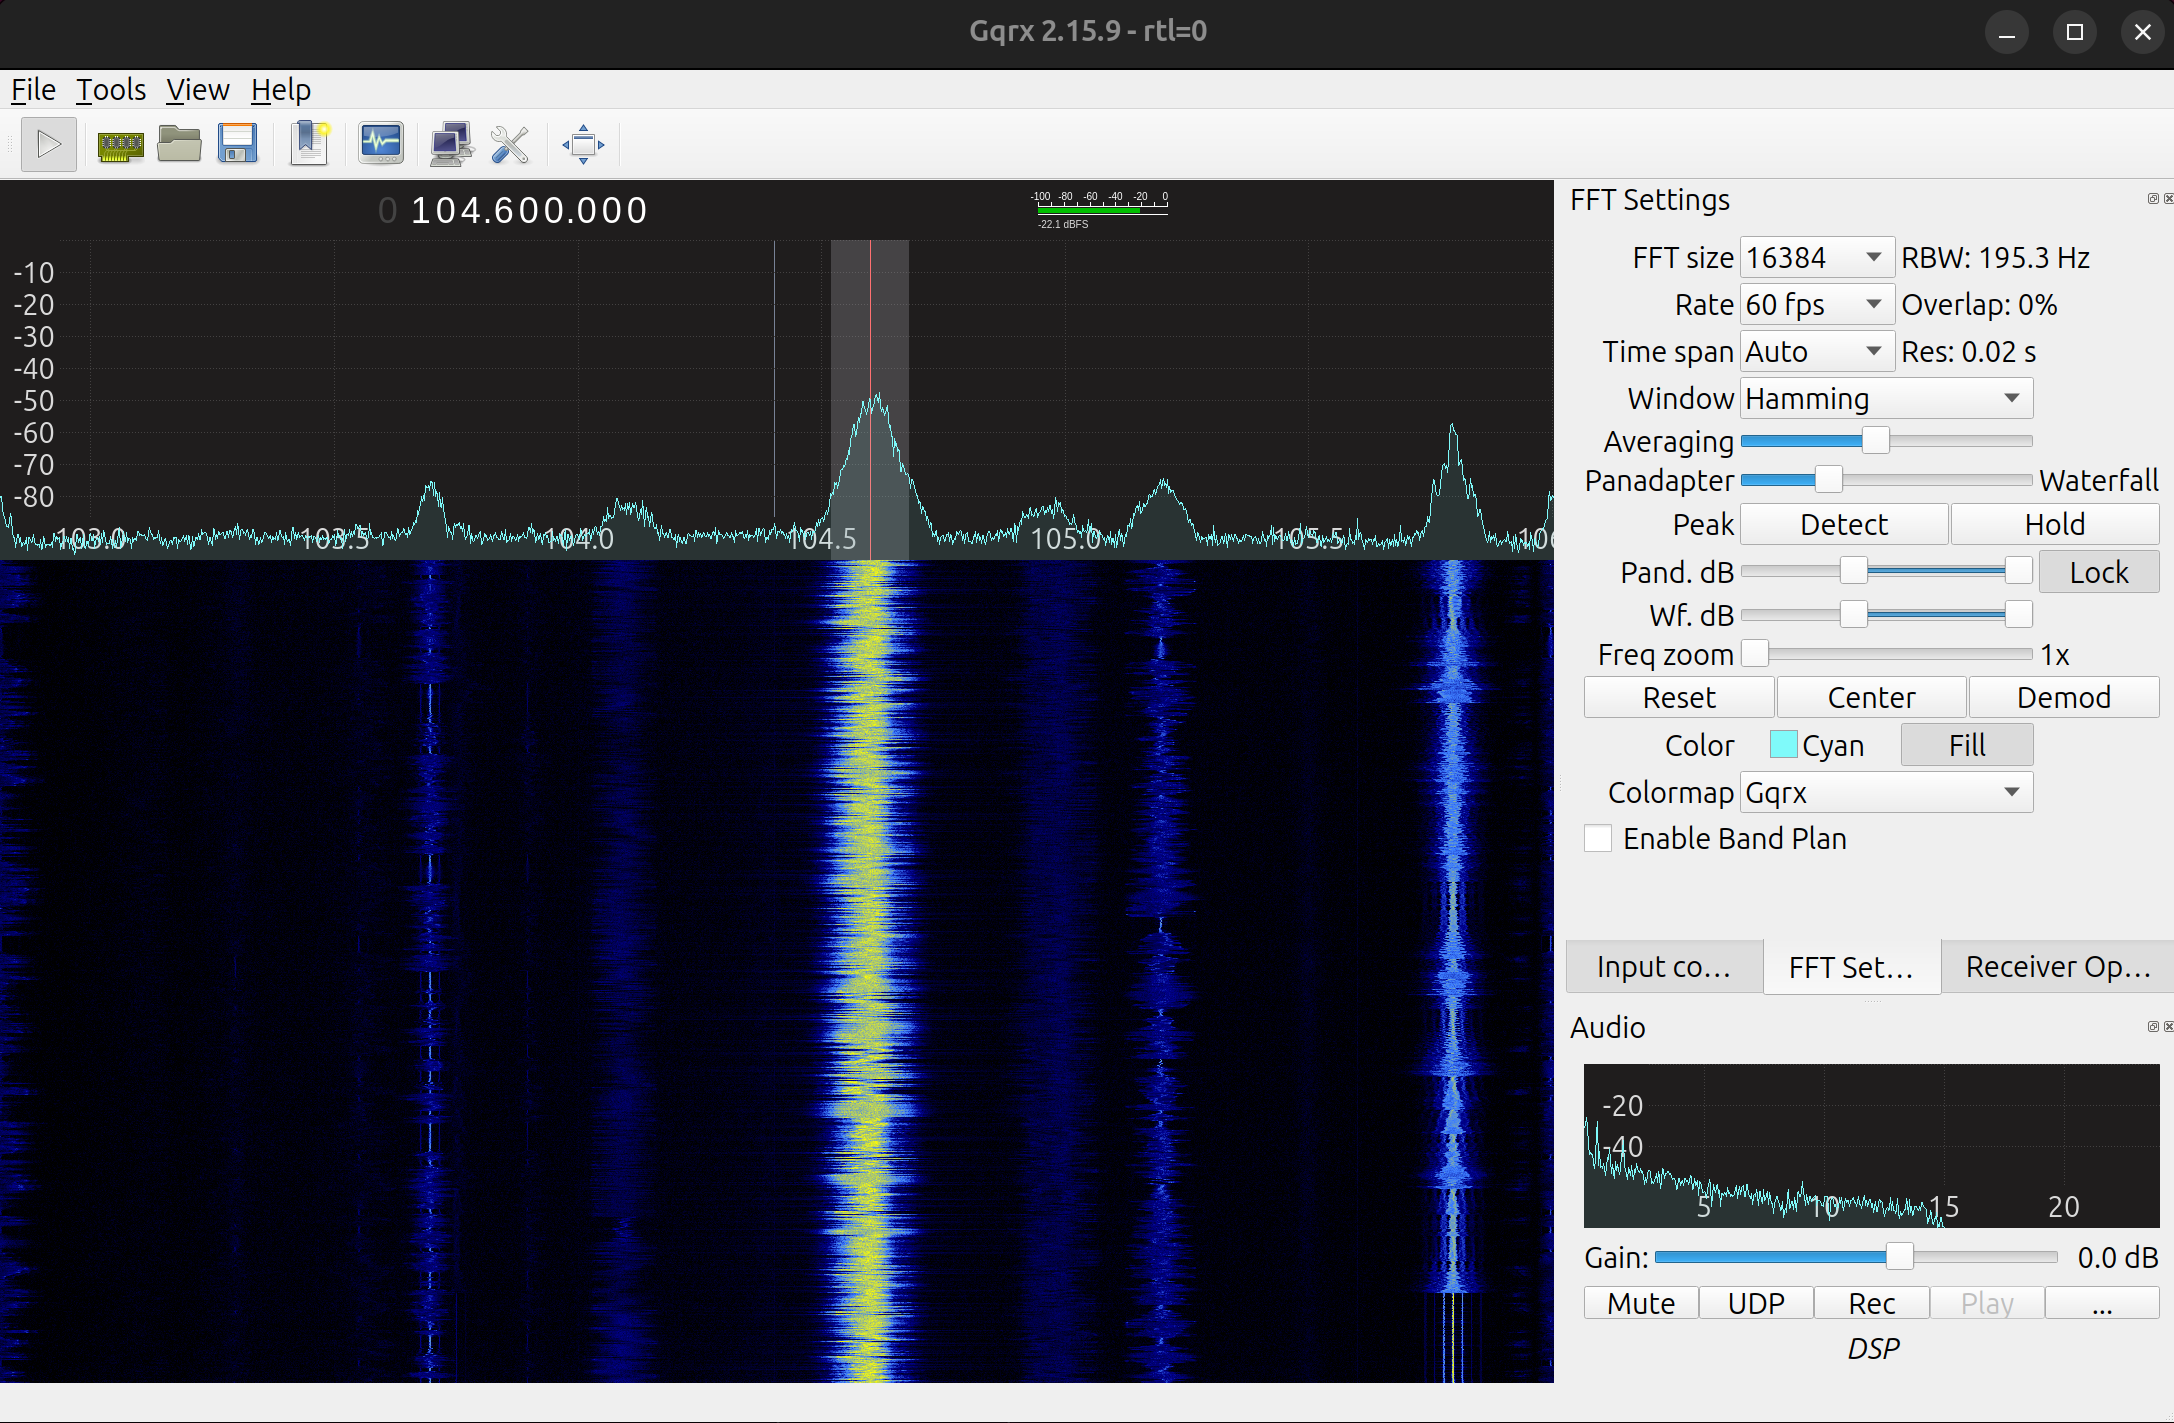
\includegraphics[scale=0.18]{images/gqrx1.png}
\caption{Réception de la station radio Classic21}\label{term38}
\end{figure}

Durant la réception du signal, il est possible de modifier l'affichage. A droite de l'affichage en spectre et en cascade sur la figure \ref{term38}, il y a différents paramètres : pour l'affichage en spectre, le paramètre \textbf{Panadapter dB} représente la force du signal des fréquences radio reçues affichées sur l'axe vertical du graphique du spectre. Pour l'affichage en cascade, le paramètre \textbf{Waterfall dB} modifie l'intensité utilisée pour afficher la force du signal, permettant ainsi d'ajuster le contraste ou la visibilité des signaux plus faibles ou plus forts. 

\vspace{0.1cm}

Les paramètres suivants sont communs et affectent les deux affichages : le paramètre \textbf{FFT size} détermine le nombre d'échantillons utilisés dans chaque calcul de la \ac{FFT}. Une valeur plus large donne un meilleure résolution, mais consomme plus de ressources. La valeur est une puissance de deux pour des raisons d'efficacité de calculs. Le paramètre \textbf{Rate} détermine le taux de rafraîchissement de l'affichage. Un taux relativement faible avec une taille de frame \ac{FFT} élevé induit un effet d'overlap, c'est-à-dire que des frames consécutives partagent des échantillons, ce qui donne un affichage plus lisse du spectre.

\newpage

\subsubsection{Universal radio hacker, URH}


\ac{URH} est un logiciel open source similaire à GQRX. Son rôle principal est l'analyse de signaux radio. Au-delà de l'écoute en temps réel, \ac{URH} peut sauvegarder des signaux et lire des enregistrements à partir de fichiers. La figure \ref{term39} montre comment enregistrer un signal. Les paramètres à configurer sont similaires à GQRX (le choix de la \ac{SDR}, la fréquence, le taux d'échantillonnage, la largeur de bande et le gain). Comme \ac{URH} est le principal outil d'analyse pour ce travail, les analyses avec ce dernier sont détaillées dans la section \ref{urh}.

\begin{figure}[h]
\centering

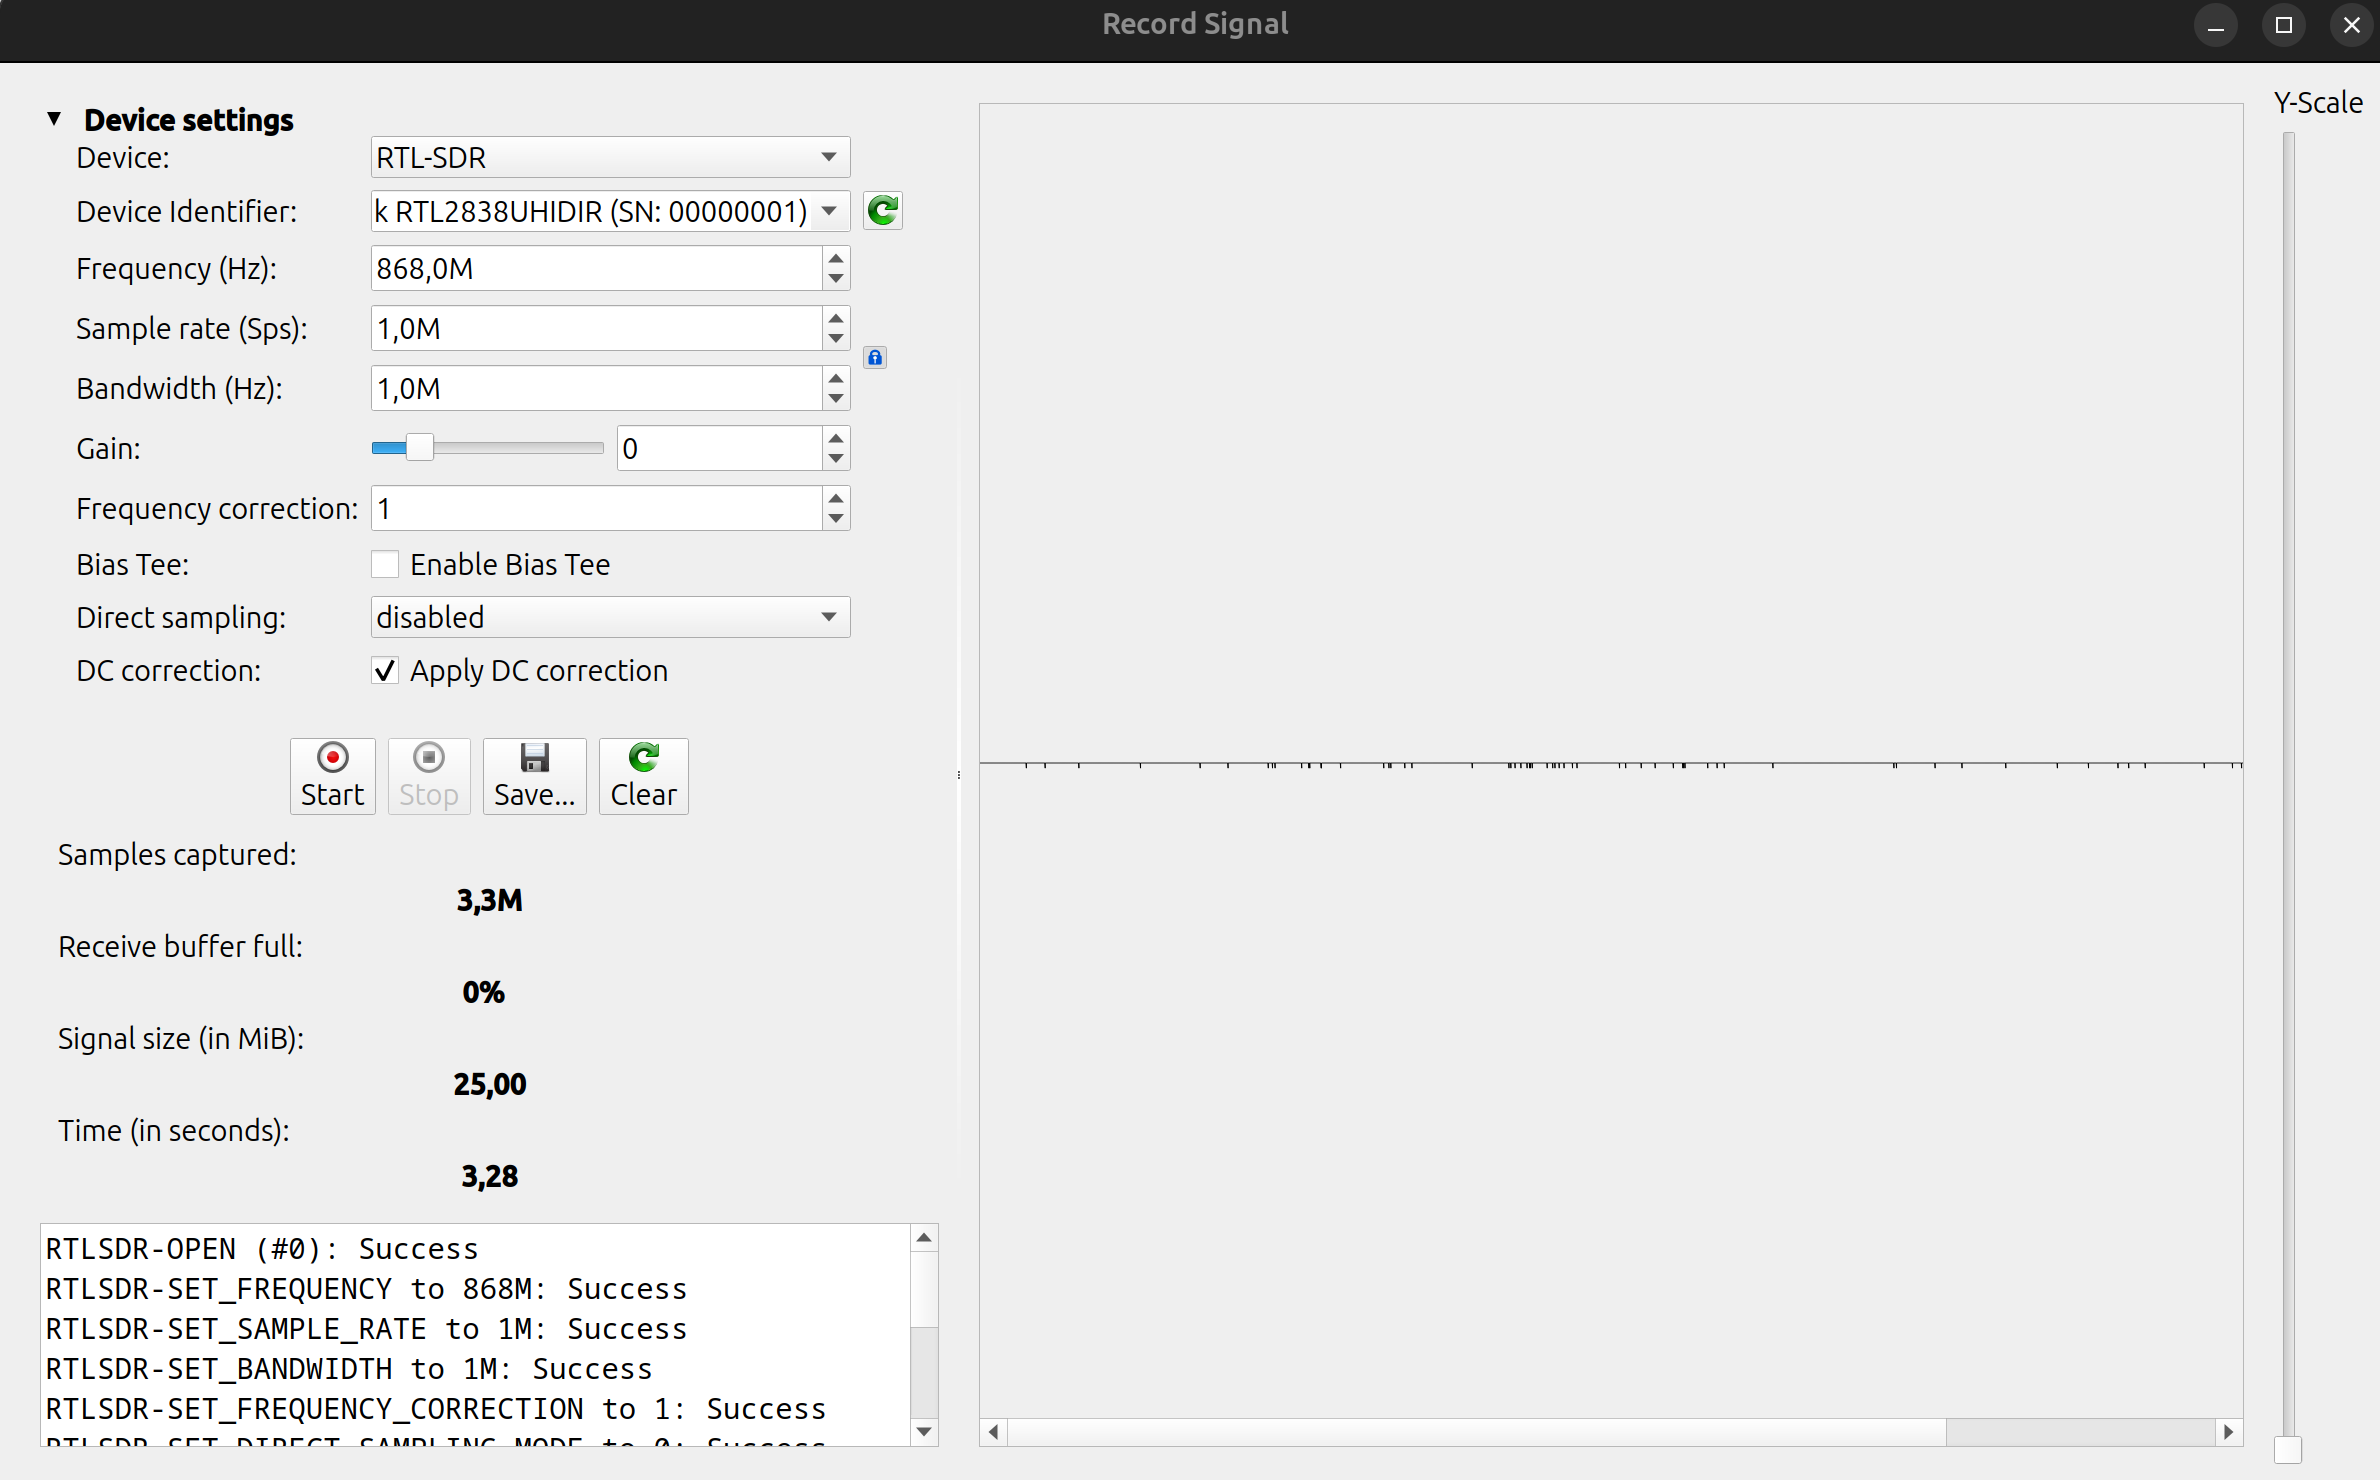
\includegraphics[scale=0.16]{images/urh1.png}
\caption{Enregistrement d'un signal avec URH}\label{term39}
\end{figure}

\newpage

Les fichiers qu'\ac{URH} peut interpréter ou enregistrer sont au format \textit{.complex}. Ce format est utilisé pour sauvegarder les signaux sous forme d'échantillons \ac{I/Q}. Il existe plusieurs variantes de ce format supportées par \ac{URH} :

\vspace{0.1cm}

\begin{table}[h]
\centering
\begin{tabular}{|c|c|c|c|}
\hline
\multicolumn{1}{|c|}{} & \multicolumn{1}{c|}{Taille I (bits)} &\multicolumn{1}{c|}{Taille Q (bits)} & \multicolumn{1}{c|}{Type}\\
\hline
.complex & 32 & 32 & float \\
\hline
.complex64 & 32 & 32 & float\\
\hline
.complex16u & 8 & 8 & unsigned int\\
\hline
.complex16s &  8 & 8 & int\\
\hline
.complex32u & 16 & 16 & unsigned int \\
\hline
.complex32s & 16 & 16 & int  \\
\hline
\end{tabular}
\caption{Table des formats supportés par URH}
\label{format}
\end{table}



\section{Python}

Le choix du langage pour l'implémentation du travail est Python (version 3.11.4). Python donne l'accès à plusieurs librairies très pertinentes pour faire du signal processing. Voici les principales librairies utilisées :

\vspace{0.1cm}

\begin{itemize}
\item Numpy. Cette librairie est fondamentale pour la gestion des arrays. Elle contient également de nombreuses fonctions et formats mathématiques utiles au projet.
\item Matplotlib. Cette librairie permet d'effectuer des plots de données de manière simple et efficace.
\item PyRTLSDR. La librairie PyRTLSDR est essentielle pour pouvoir manipuler la \ac{SDR} R820T2. Il est possible de configurer la \ac{SDR} sans devoir passer par un software tiers comme GQRX ou \ac{URH} grâce à cette librairie.
\item PyHackRF. L'équivalent de PyRTLSDR mais pour la \ac{SDR} HackRF One.
\item Datashader. Cette librairie permet la visualisation améliorée de grande quantité de données via l'ajout de gradient coloré.
\item Serial. La manipulation des modules rn2483 est possible grâce à la librairie serial. Cette librairie permet d'interagir avec les appareils connectés via USB.
\end{itemize}

\newpage

L'environnement de travail utilisé est Visual Studio Code (version 1.87.1). Cet \ac{IDE} est open source et largement populaire, ce qui permet un apprentissage très rapide pour des travaux spécifiques via Internet. L'utilisation de VSCode est motivée par son système d'extension, qui contient plusieurs extensions qui permettent de manipuler directement les modules d'émission \ac{LoRa}. Le module LoPy de Pycom est compatible avec VSCode via l'extension PyMakr. GitHub est également intégré dans VSCode, ce qui permet de simplifier la mise en ligne du travail. La table \ref{table2} donne une comparaison des différents logiciels basée sur plusieurs critères.

\begin{table}[h]
\centering
\begin{tabular}{|p{4cm}|p{2cm}|p{2cm}|p{3.5cm}|}
\hline
\multicolumn{1}{|c|}{} & \multicolumn{1}{c|}{GQRX} & \multicolumn{1}{c|}{URH} & \multicolumn{1}{c|}{Python}\\
\hline
Interface Utilisateur & GUI avec affichage en temps réel & GUI avec outils plus poussés pour analyse & Pas de GUI \\
\hline
Réception de signaux & \multicolumn{3}{c|}{oui} \\
\hline
Génération de signaux & non & \multicolumn{2}{c|}{oui} \\
\hline
Sauvegarde des données & pas de sauvegarde possible & \multicolumn{2}{c|}{sauvegarde et chargement possibles} \\
\hline
Format des données & / & voir table \ref{format} & .complex64 jusqu'à .complex512 \\
\hline
Démodulation &  \multicolumn{2}{c|}{les plus communes\footnotemark[12]}  & toutes\\
\hline
Courbe d'apprentissage & prise en main très rapide & prise en main rapide & plus de possibilités donc plus de temps d'apprentissage \\
\hline
Analyse du signal & concentrée sur le temps réel & \multicolumn{2}{c|}{concentrée sur l'analyse en profondeur} \\
\hline
SDR supportées & \multicolumn{3}{c|}{toutes les SDR présentées} \\
\hline
\end{tabular}
\caption{Table comparative des logiciels utilisés}
\label{table2}
\end{table}

\footnotetext[12]{AM, FM, PM, ASK, FSK, PSK, CW, CSS}

GQRX offre globalement de meilleurs outils pour la visualisation en temps réel, là où \ac{URH} permet l'analyse de manière plus précise et avec plus de possibilités. Python permet une customisation encore plus poussée à condition de manuellement rajouter ces fonctionnalités.

\newpage

\section{Géneration et réception d'un signal LoRa} \label{signallora}

La première étape de l'expérimenation consiste à générer, via un module, un signal \ac{LoRa} et à le capturer à l'aide d'une radio logicielle. Pour cette première étape, le module d'émission choisi est le module RN2483, car il est le plus facile et rapide à configurer.
Via Python, il est possible d'utiliser la librairie Serial pour se connecter au port \ac{USB} reliant le module à l'ordinateur. Ensuite, via les différentes commandes, on configure le module en modifiant les paramètres suivants : 

\vspace{0.1cm}

\begin{itemize}
\item la modulation, en LoRa.
\item La fréquence. 868MHz, la fréquence de la bande \ac{ISM} , la bande d'émission en Europe.
\item La largeur de bande ou \ac{BW} choisie est de 125KHz, ce qui est la plus petite valeur possible que permet le module.
\item La puissance du module, au maximum (14dBm).
\item Le spreading factor, la valeur la plus grande possible est choisie (SF = 12).
\item Le \ac{CR}. Il y a 4 valeurs possibles: 4/5, 4/6, 4/7 and 4/8. Cela signifie que tout les 4 bits seront codés par 4, 5, 6, 7 ou 8 bits de transmission en fonction de cette valeur. Plus la valeur est faible (la plus faible étant 4/8), plus le \ac{TOA} sera élevé, car cela prend plus de temps pour transmettre le message.
\item Le message à envoyer. Le but de cette expérimentation n'est pas de récupérer l'information initiale (le contenu du message), il n'a donc pas un grand intérêt. Le message à envoyer est un nombre hexadécimal : $0x1509ACF$.
\end{itemize}

\vspace{0.1cm}

Le choix des valeurs pour les différents paramètres a pour but de maximiser le \ac{TOA}. Les commandes relatives à la configuration sont disponibles dans l'annexe \ref{codern}

\subsection{Analyse avec GQRX}

Une fois que le module est configuré, il faut paramétrer le récepteur, la radio logicielle. La \ac{SDR} choisie est la RTL-SDR T820R2. Voici les paramètres de la \ac{SDR}:

\vspace{0.1cm}

\begin{itemize}
\item la fréquence. La fréquence d'écoute, idéalement la même fréquence de celle de l'émetteur (868MHz).
\item Le taux d'échantillonnage. Il est possible de choisir la quantité d'échantillons traités chaque seconde. Un taux plus élevé donnera un signal plus complet.
\item Le gain. Dépendant de la qualité du signal, il peut être nécessaire d'ajouter du gain, c'est à dire d'amplifier la force du signal. Un gain trop élevé peut saturer le signal, c'est-à-dire quand l'amplitude dépasse la portée du récepteur.
\end{itemize}

\vspace{0.1cm}

La figure \ref{term301} montre la capture de deux signaux LoRa. On remarque que malgré la configuration des paramètres pour maximiser le \ac{TOA}, il est difficile d'observer en détail le signal. On observe également que le signal se situe entre la fréquence 867.915MHz et 868.040MHz, ce qui correspond bien à la largeur de bande de 125KHz choisie.

\begin{figure}[h]
\centering

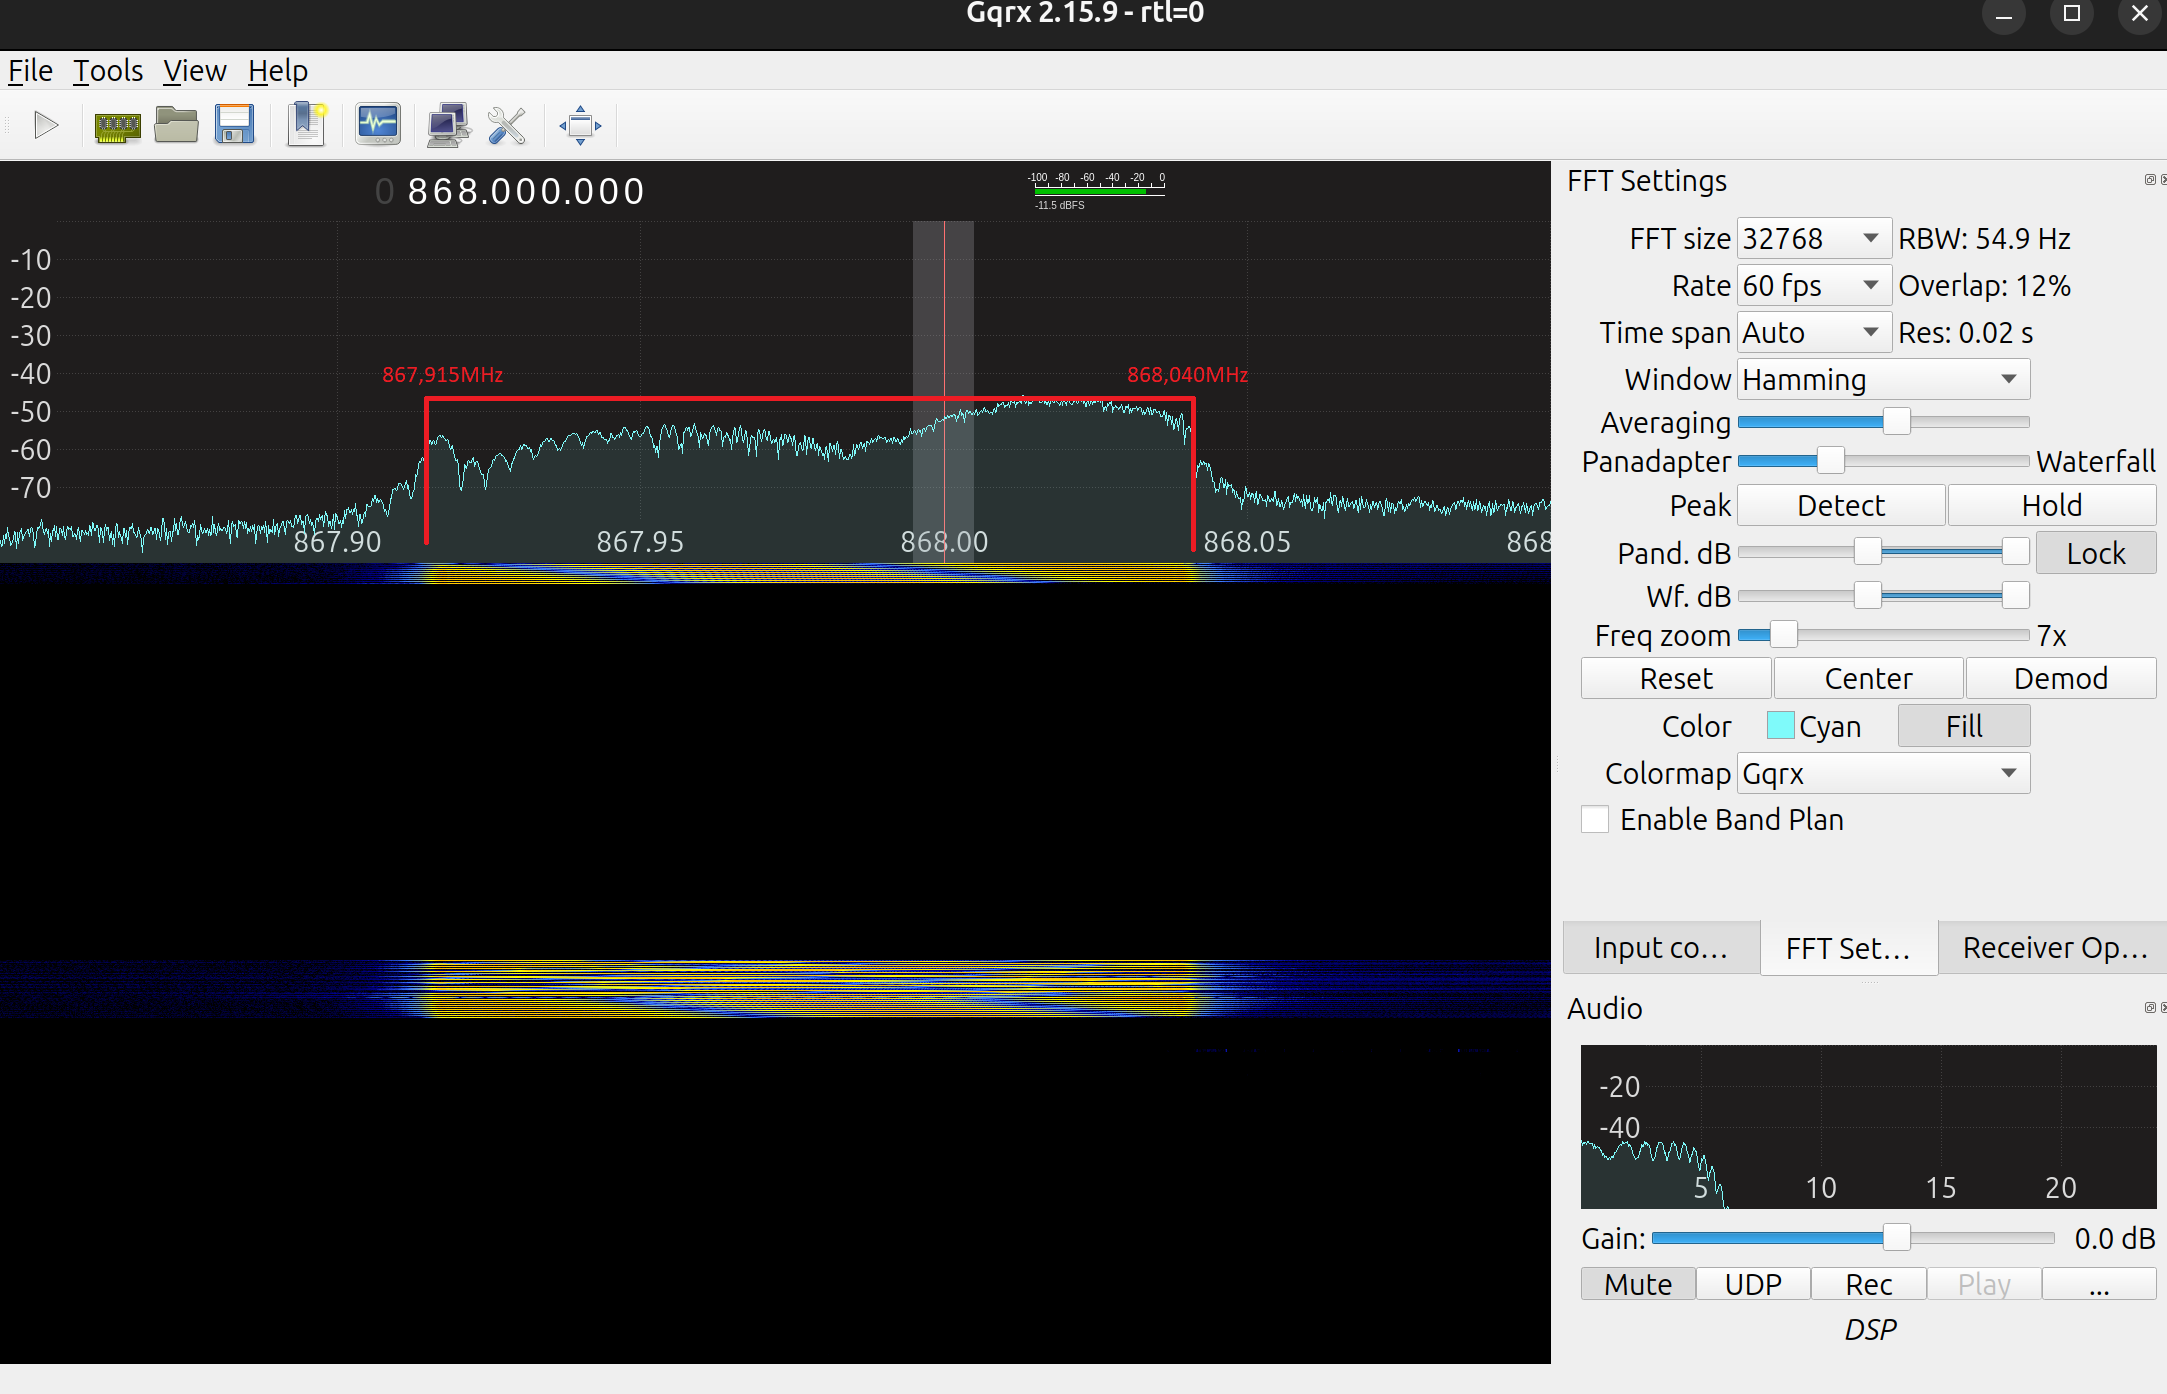
\includegraphics[scale=0.28]{images/gqrx4.png}
\caption{capture module rn2483 sur GQRX avec RTL-SDR R820T2. Sample rate = 1.8MHz}\label{term301}
\end{figure}

Le module Arduino, contrairement aux modules Pycom et RN2483, permet d'utiliser une largeur de bande beaucoup plus faible. La figure \ref{term302} montre la capture d'un signal \ac{LoRa} émis depuis le module Arduino. La largeur de bande choisie est de 7.8KHz, les autres paramètres d'émission (la modulation, la fréquence et le spreading factor) sont similaires à ceux de la capture précédente. Cette fois-ci, on distingue clairement sur l'affichage en spectre un pic à 868.070MHz. Sur l'affichage en cascade, le signal se dessine sous forme de traits (les chirps). Cela correspond bien à la théorie de la modulation \ac{LoRa} où le signal modulé est composé de upchirps et downchirps. Il y a, de part et d'autre du signal, des silhouettes. Cela est dû à la sensibilité de la \ac{SDR}: si on observe les pics de fréquences dans l'affichage en spectre, on constate qu'ils sont négligeables car leurs échelles de puissances sont bien inférieures (environ 60dB plus faible) à celle du pic principal. GQRX permet de visualiser le signal, mais pour pousser l'analyse plus en détails, l'utilisation d'Universal Radio Hacker est nécessaire.

\begin{figure}[h]
\centering

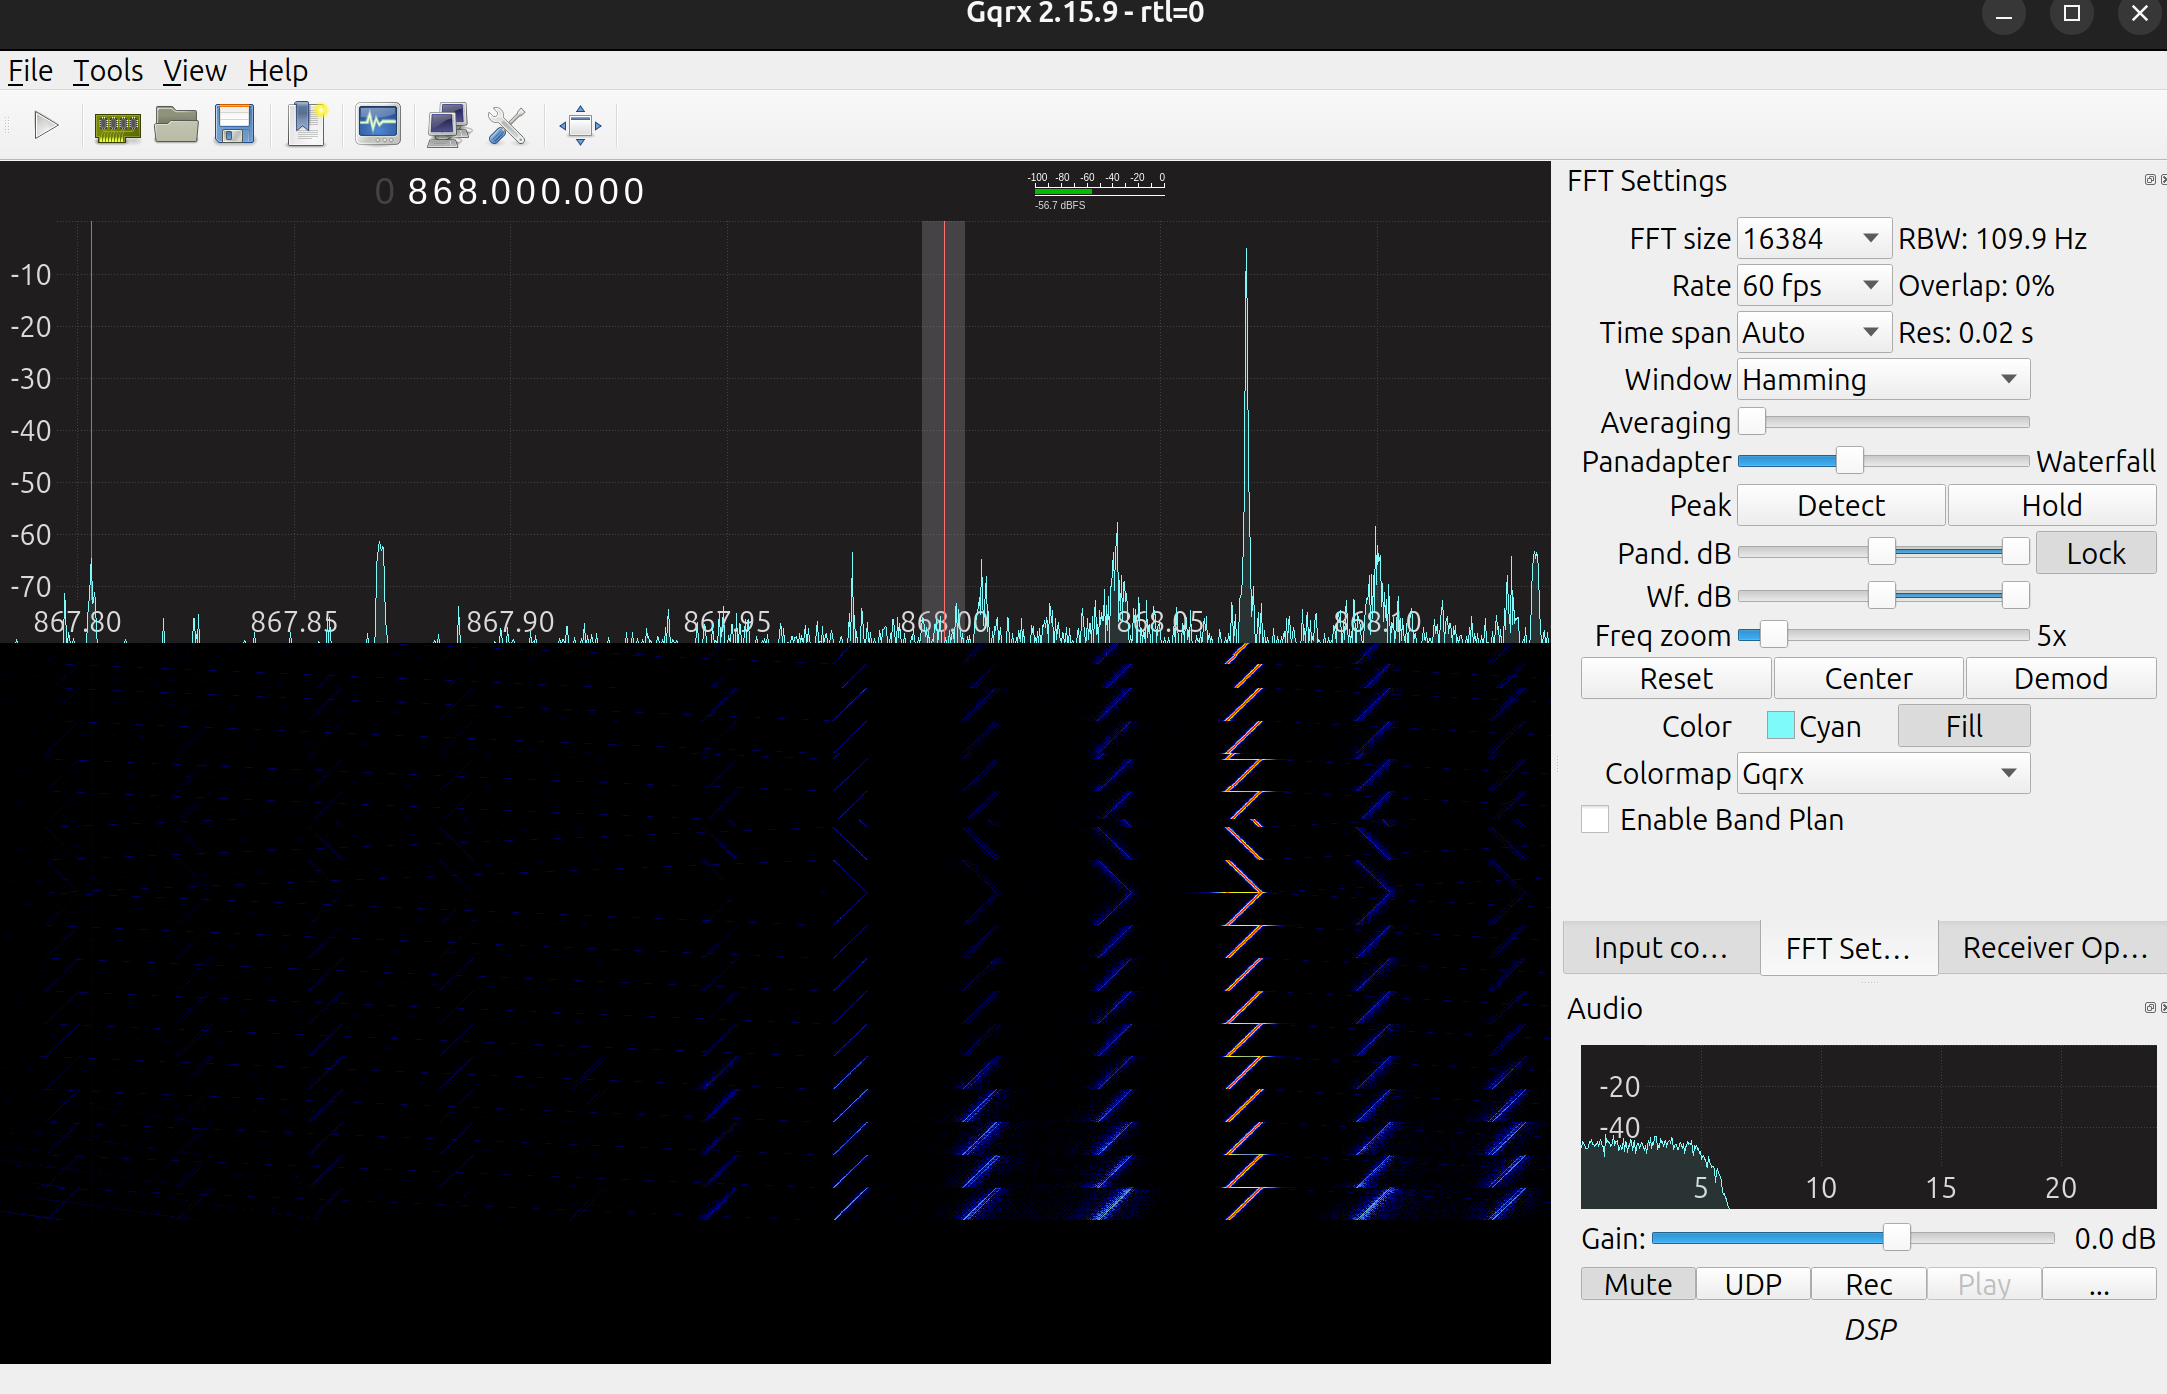
\includegraphics[scale=0.17]{images/gqrx5.png}
\caption{capture module Arduino sur GQRX avec RTLSDR R820T2 Sample rate = 1.8MHz}\label{term302}
\end{figure}


\subsection{Analyse avec URH}\label{urh}

GQRX permet de zoomer sur les fréquences mais pas sur le temps, ce qui demande donc de générer un signal dont le \ac{TOA} doit être le plus élevé possible. \ac{URH} offre plus de flexibilité sur l'analyse ce qui permet de ne pas devoir utiliser des largeurs de bande aussi faibles que celles du module Arduino. Ainsi, pour l'analyse avec \ac{URH}, les modules Pycom et RN2483 sont utilisés. La figure \ref{term303} et \ref{term304} montre la capture et la sauvegarde d'un signal LoRa. Le module utilisé est rn2483, la \ac{SDR} est la R820T2. les paramètres d'émission sont les suivants : \ac{BW} = 125KHz, \ac{SF} = 8, fréquence = 868MHz, Mode = \ac{LoRa}, \ac{CR} = 4/8, power = 14. Les paramètres du récepteur sont les suivants : fréquence = 868MHz, \ac{SR} = 1.8MHz, gain = 0dB. Pour des raisons de simplicité, le signal capturé avec ses paramètres sera utilisé comme référence pour toute la partie analyse jusqu'à la fin de la section \ref{signallora}.

\newpage

\begin{figure}[h]
\centering

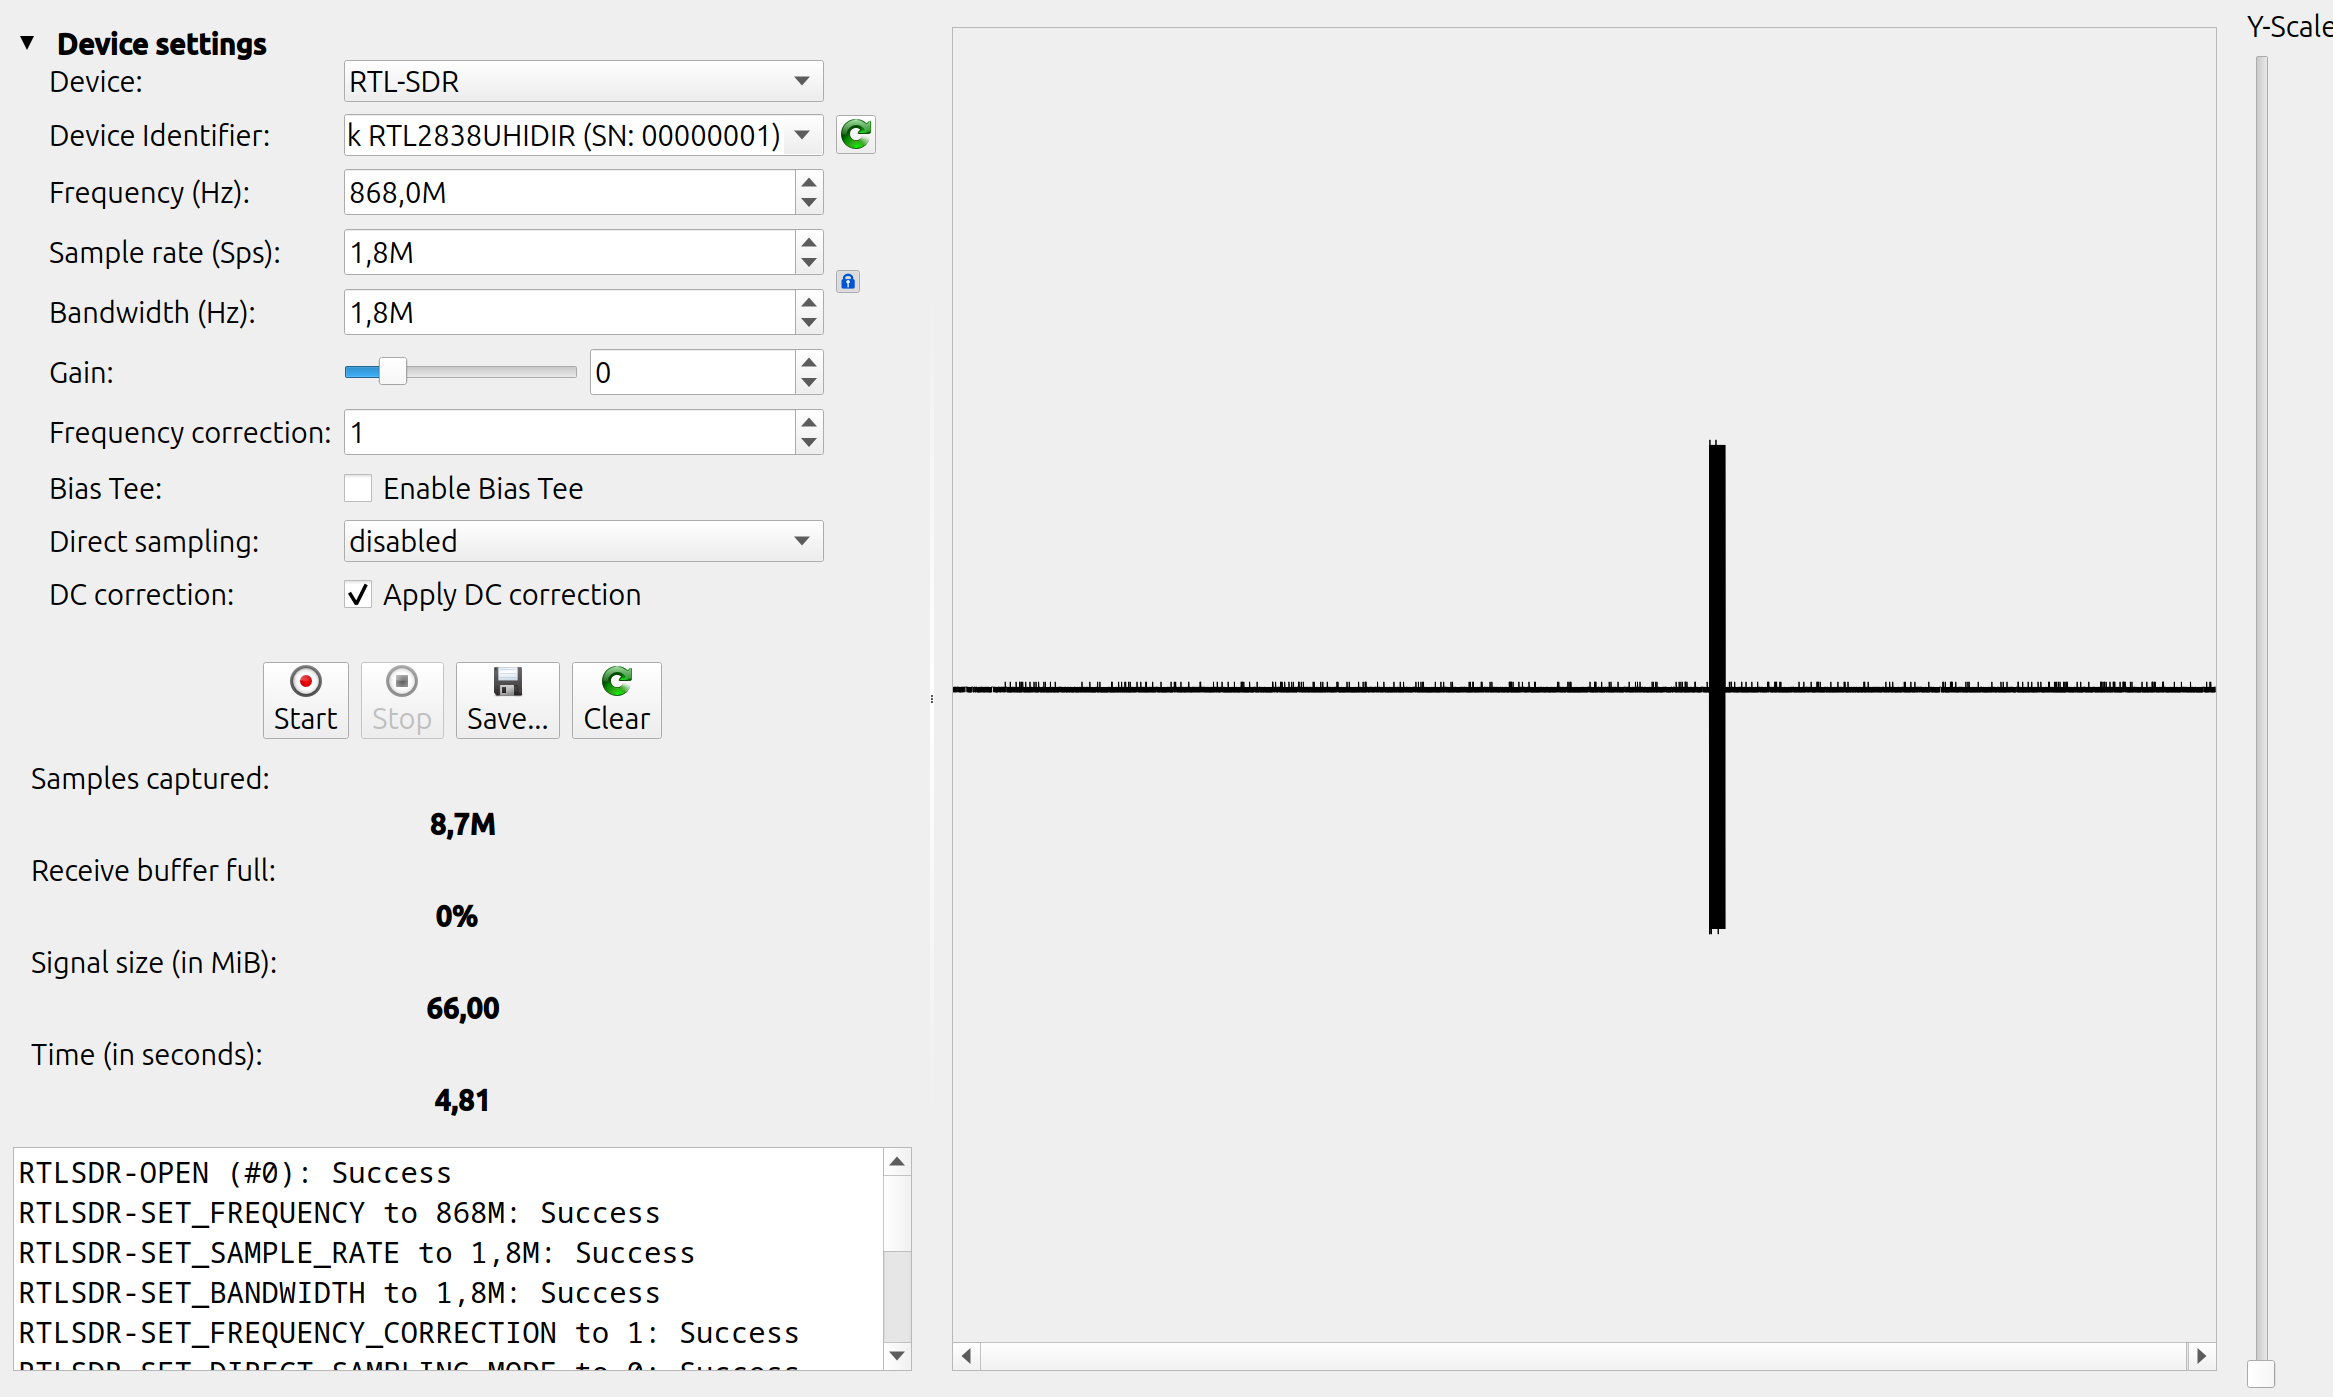
\includegraphics[scale=0.17]{images/urh2n.png}
\caption{Capture du signal}
\label{term303}
\end{figure}

\begin{figure}[h]
\centering

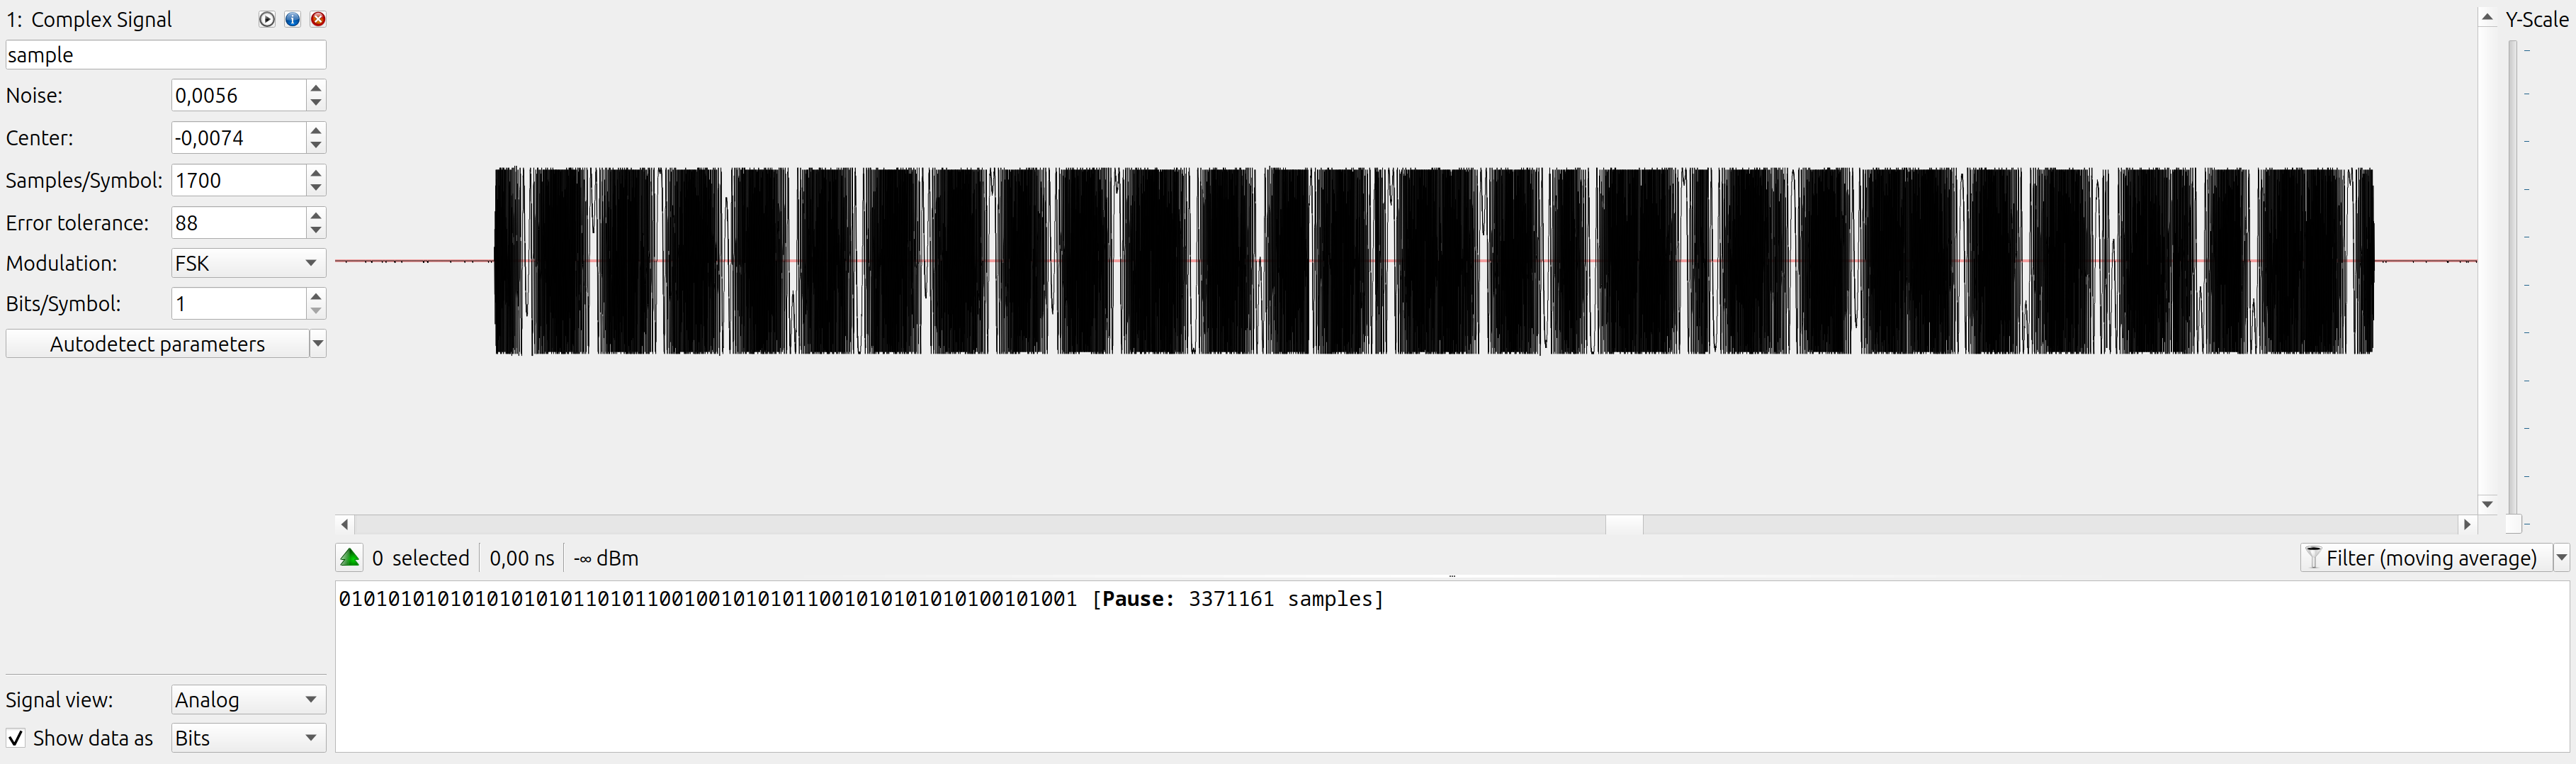
\includegraphics[scale=0.11]{images/urh3n.png}
\caption{Sauvegarde du signal}
\label{term304}
\end{figure}

A partir de la figure \ref{term304}, il est possible de couper une partie de l'enregistrement, notamment celle qui ne contient pas le signal. \ac{URH} permet également d'afficher le signal sous forme de spectrogramme, la figure \ref{term306} montre le signal sous sa forme analogique et sous spectrogramme. On constate cependant que les deux affichages ne correspondent pas. En effet, si on se fie au spectrogramme, la fréquence devrait augmenter durant le premier chirp. Or, quand on zoome sur le signal sur l'affichage analogique, celle-ci diminue dans un premier temps. (voir figure \ref{term307}).

\newpage

\begin{figure}[h]
\centering

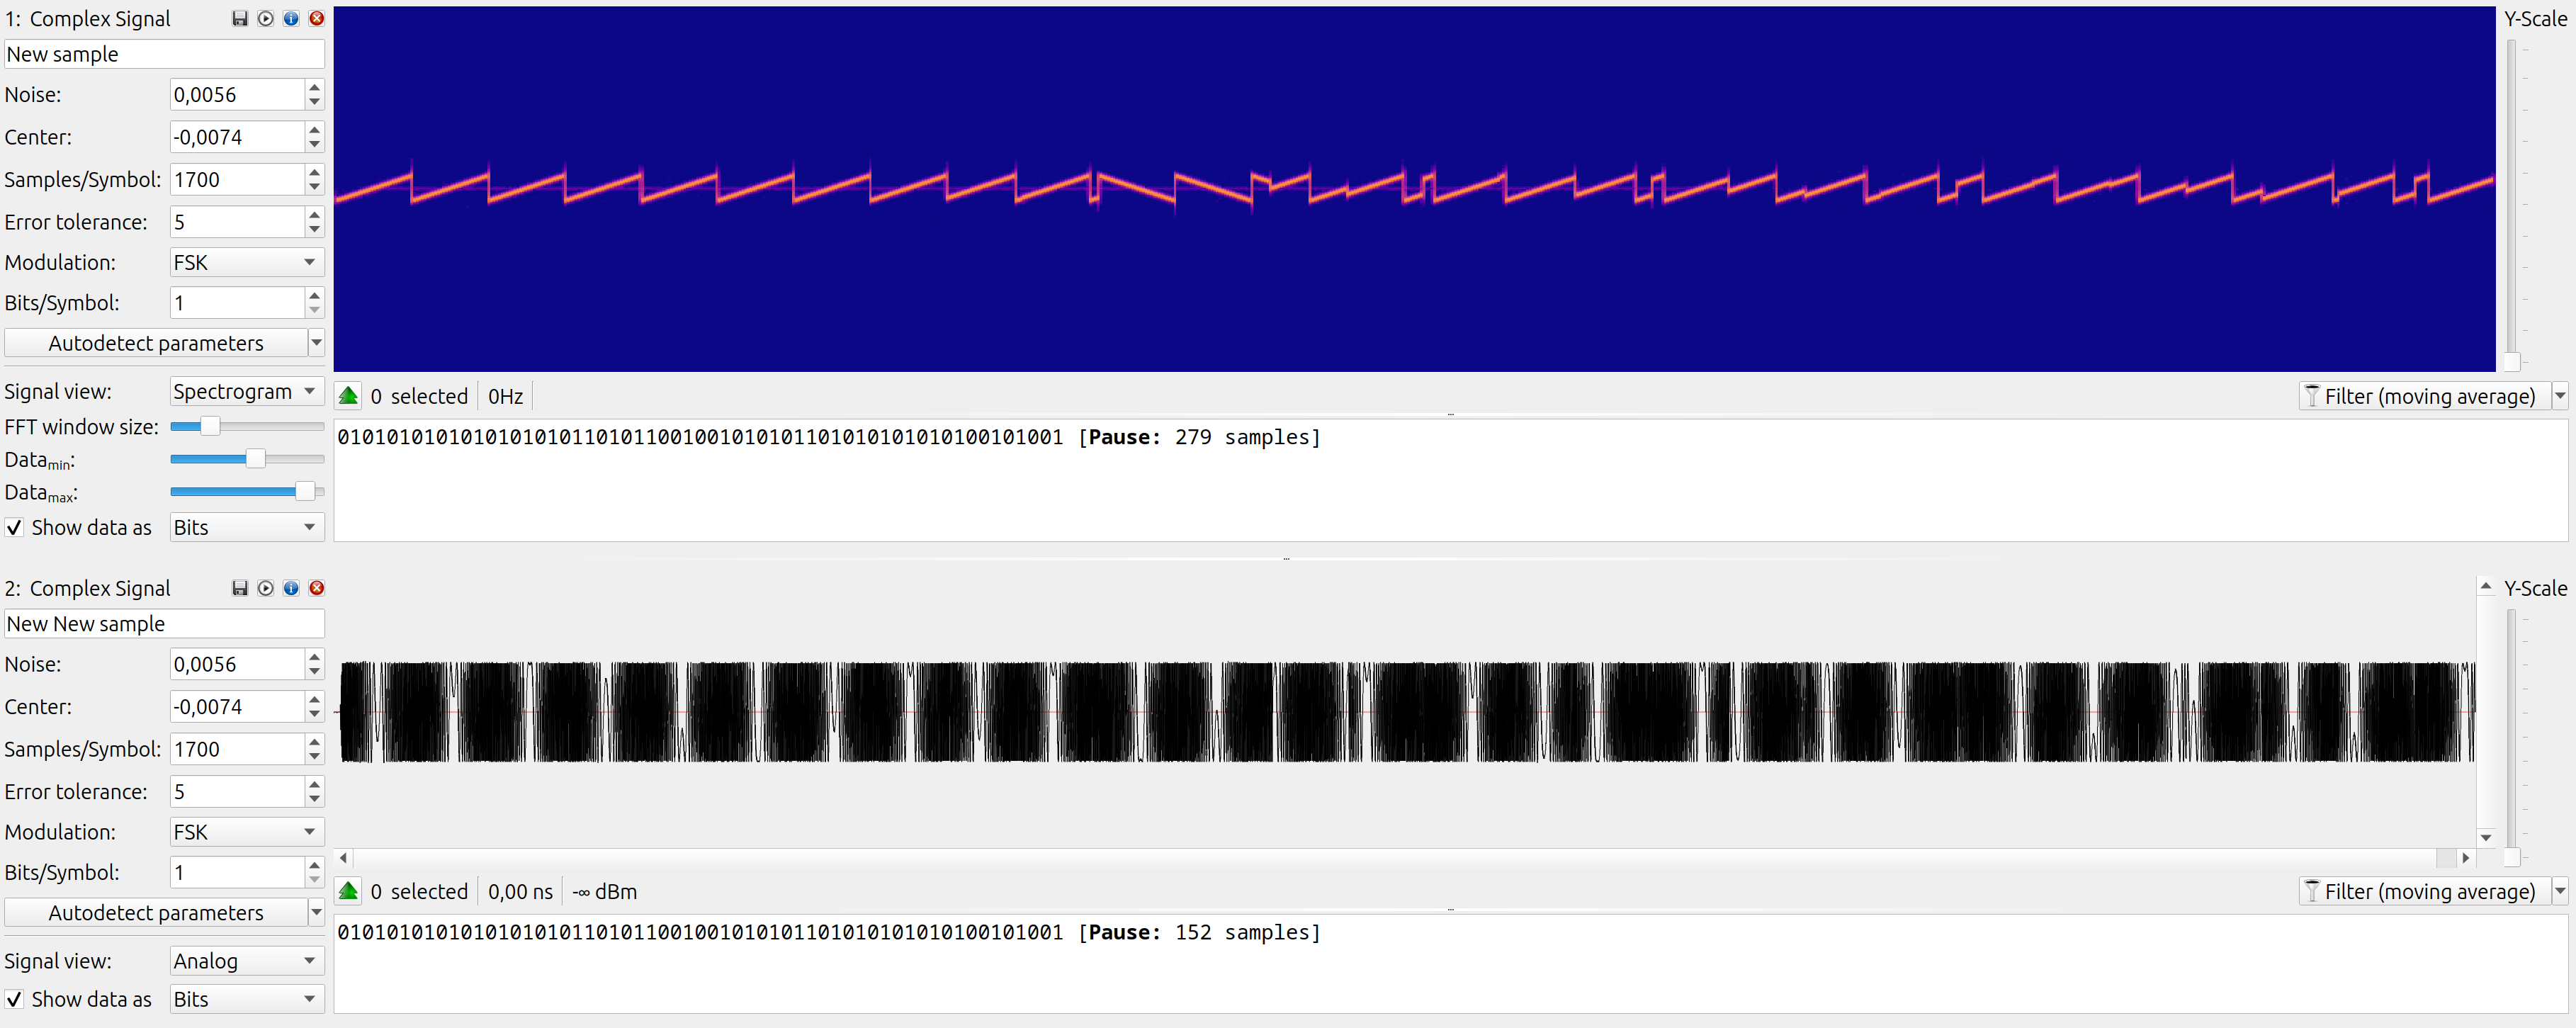
\includegraphics[scale=0.11]{images/urh4.png}
\caption{Signal LoRa sous forme spectrogramme et analogique}\label{term306}
\end{figure}

\begin{figure}[h]
\centering

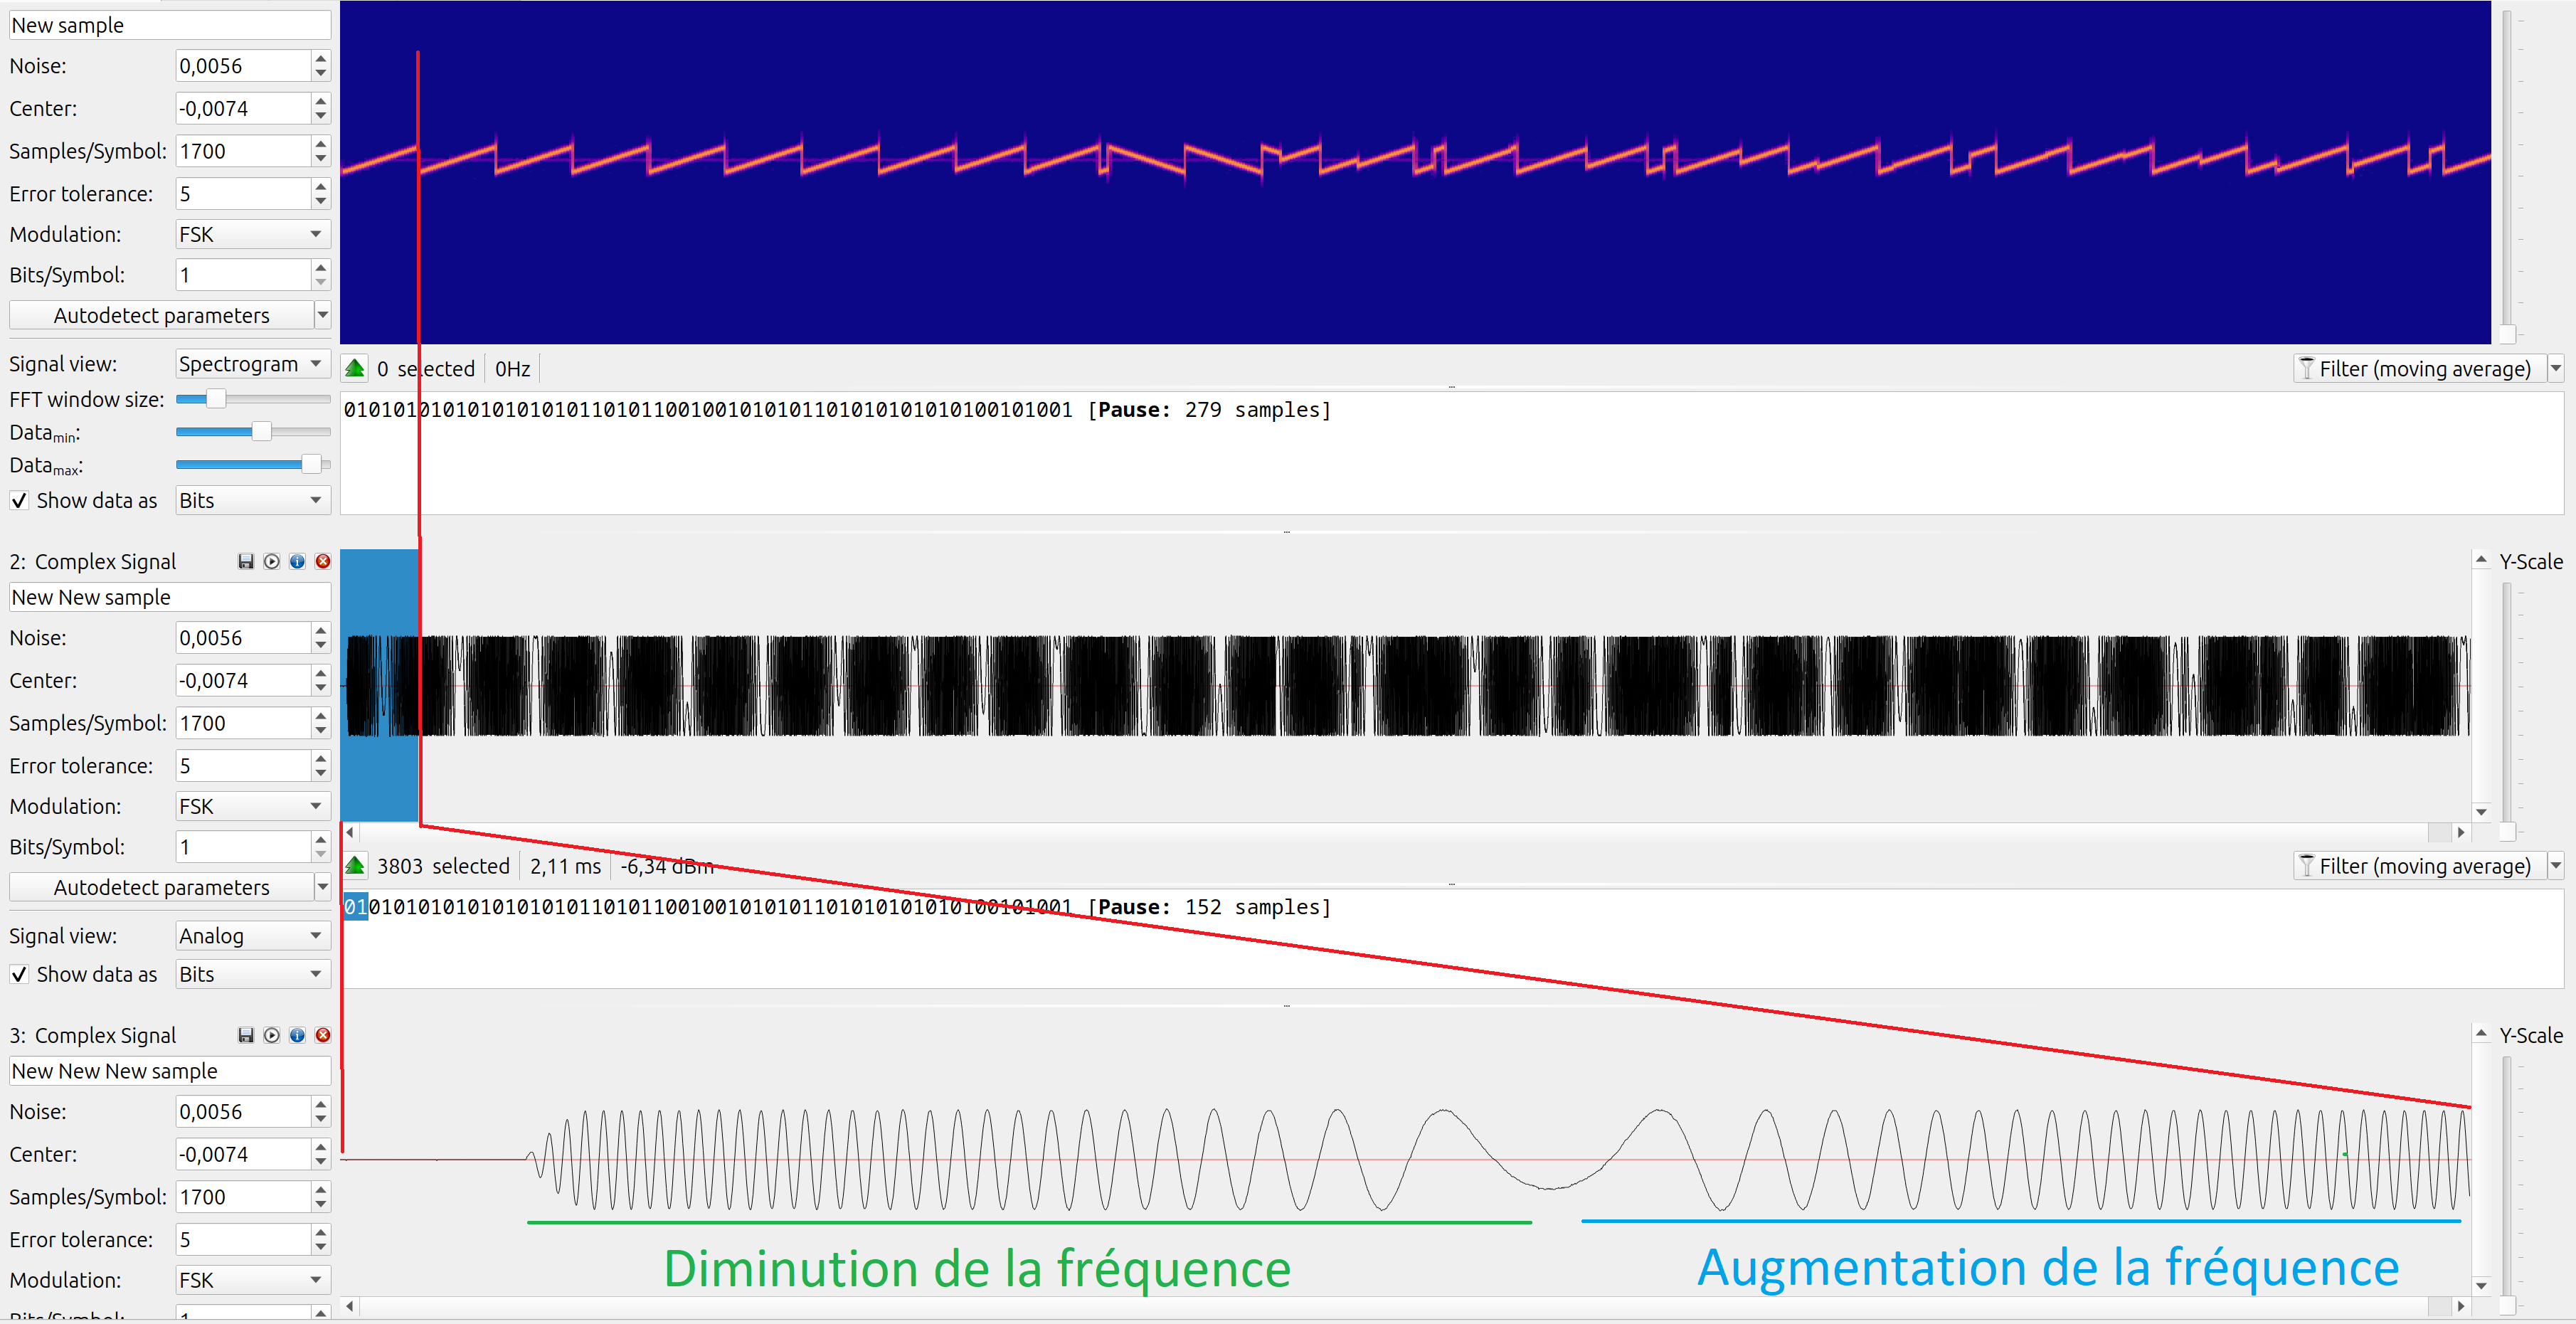
\includegraphics[scale=0.18]{images/urh5.png}
\caption{Zoom d'un upchirp du signal LoRa capturé}\label{term307}
\end{figure}

Ce phénomène est dû à une interprétation faussée par \ac{URH}. La fréquence du récepteur choisie étant la même que celle de l'émetteur, \ac{URH} va interpréter 868MHz comme étant la fréquence centrale ayant pour valeur 0, ce qui signifie que pour un signal reçu à 868MHz, la moitié des échantillons sont interprétés comme ayant une fréquence "négative". Autrement dit, \ac{URH} affiche la position inverse des échantillons qu'il considère comme négatifs. Pour éviter cette erreur, il suffit de décaler la fréquence d'écoute proportionnellement à la moitié de la taille de la largeur de bande du signal émis. Dans ce cas, le signal émis à une largeur de bande de 125KHz, il faut ajuster la fréquence d'écoute :

\begin{align}
    F_{recepteur} = F_{emetteur} - \frac{BW}{2} soit: \\
    868MHz - \frac{125KHz}{2} = 867.9375MHz
\end{align}

On observe également, au début du premier chirp, une période où l'amplitude est en train de s'ajuster. Ce phénomène, appelé période transitoire (transient part), est un état instable durant lequel différentes propriétés du signal peuvent subir des changements. Sur la figure \ref{term307}, cela survient au début de la réception, ce qui peut s'expliquer par le fait que le module d'émission change d'état au moment de débuter la transmission.

\vspace{0.1cm}

Selon la section \ref{packetlora}, la structure du paquet \ac{LoRa} devrait contenir d'abord les symboles du préambule, soit 8 upchirps suivis de 4.25 chirps. La figure \ref{term308} montre le spectrogramme du signal complet, dont la partie fixe du préambule (les 8 upchirps par défaut) ont été mis en évidence sous forme analogique. Pouvoir identifier et récupérer le préambule du signal \ac{LoRa} est crucial pour l'identification de l'appareil qui l'a émis.


\begin{figure}[h]
\centering

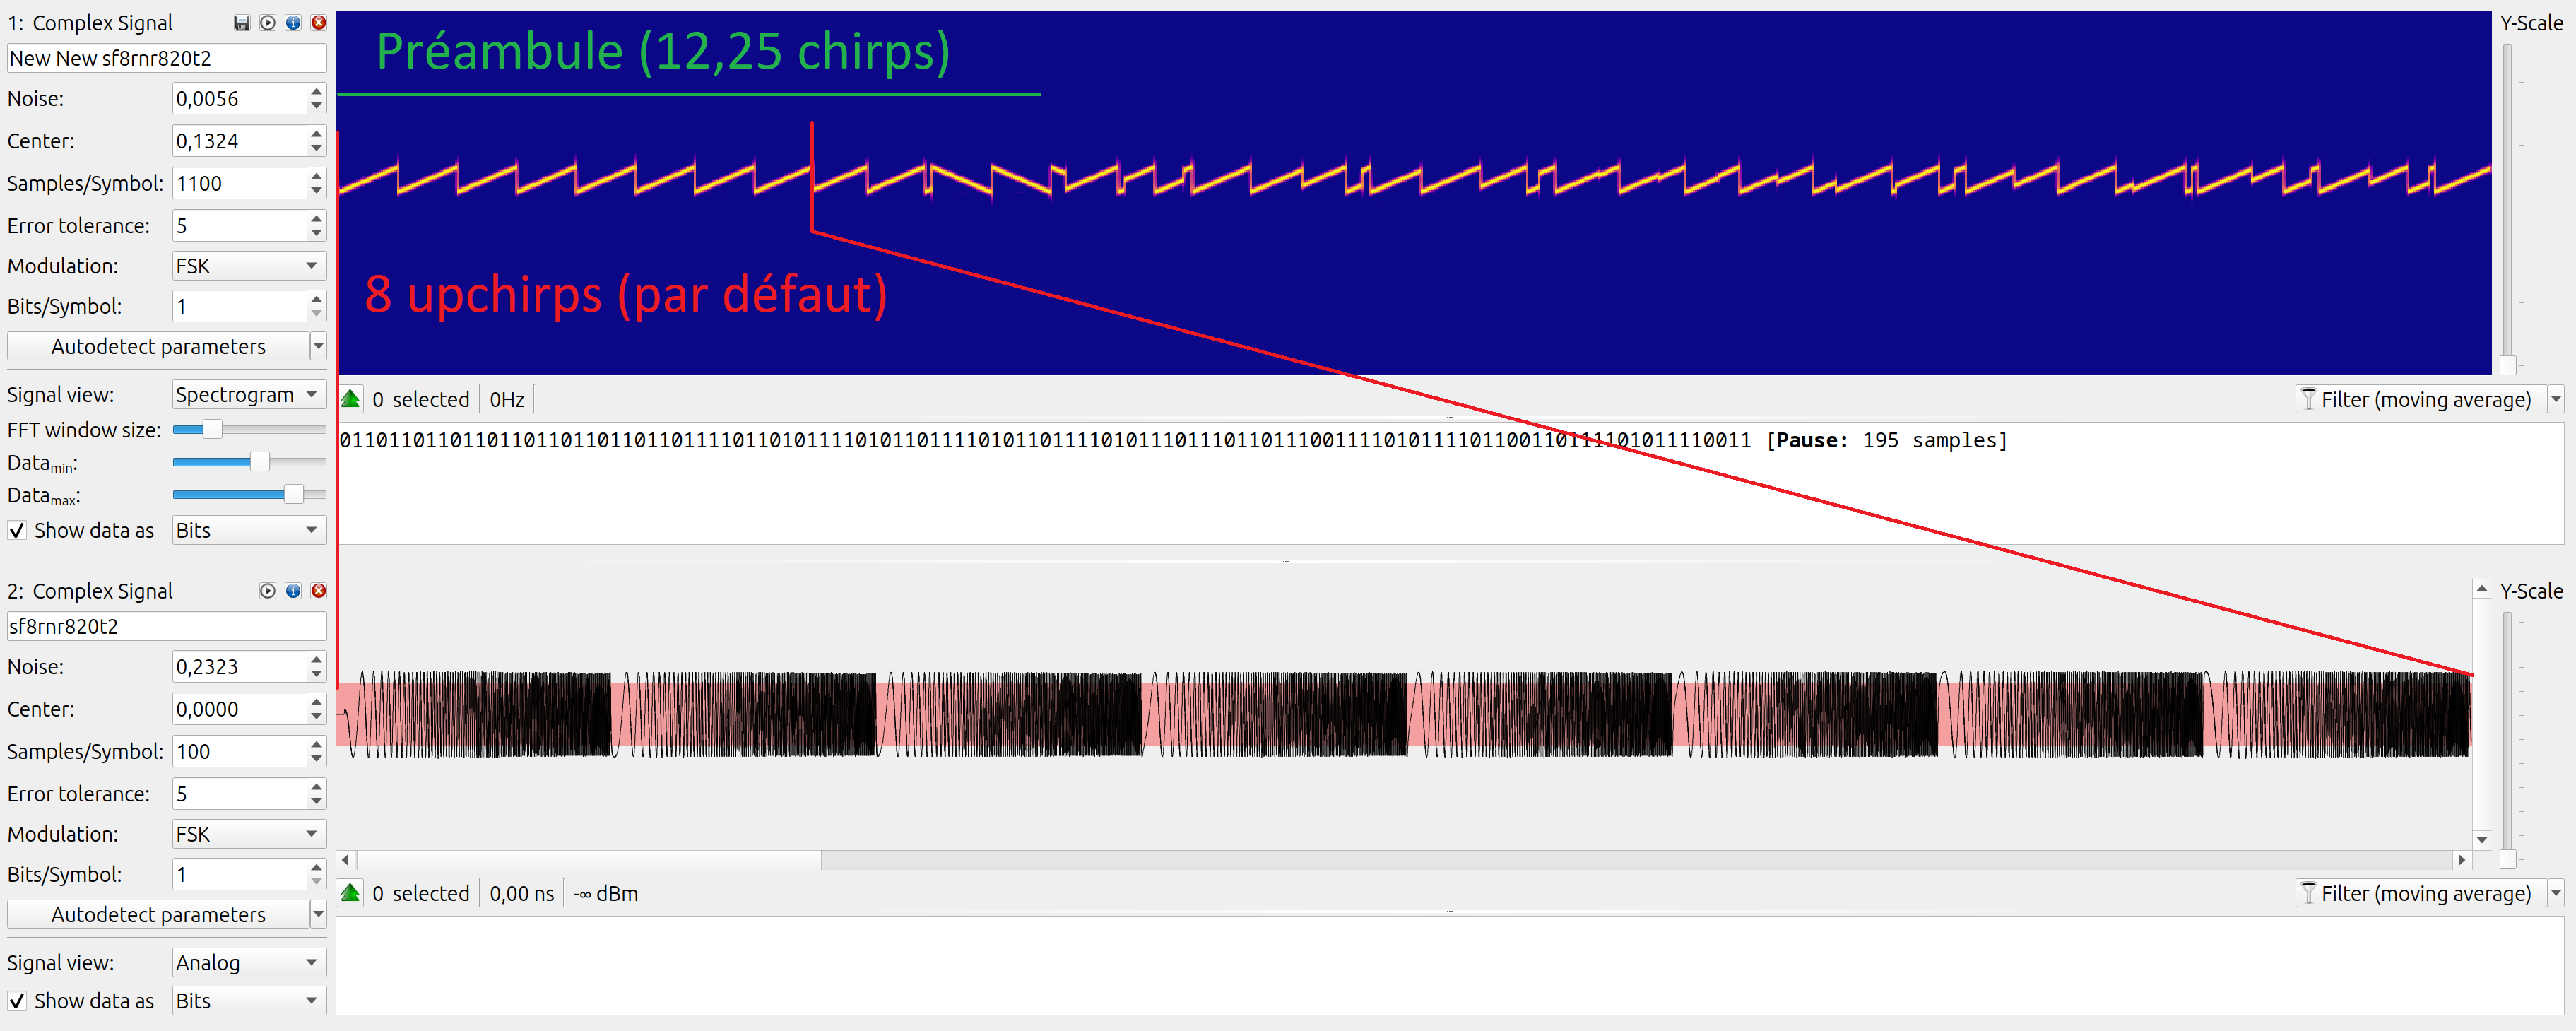
\includegraphics[scale=0.18]{images/urh6.png}
\caption{Identification du préambule LoRa}\label{term308}
\end{figure}

Cependant, l'utilisation d'intermédiaires comme \ac{URH} ou GQRX n'est pas efficace pour traiter un grand nombre de signaux. La dernière étape avant de commencer l'identification des noeuds à partir des signaux est d'automatiser le processus complet de la capture du signal. Bien qu'\ac{URH} et GQRX ne soit pas nécessaires pour réaliser l'identification, leur utilisation a été d'une grande aide: par exemple pour l'apprentissage de la reconnaissance de signaux \ac{LoRa} et de leur représentation, mais également pour l'observation de la partie transitoire d'un signal. Ils ont également permis de visualiser l'impact de paramètres comme le taux d'échantillonnage, le facteur d'étalement ou encore la largeur de bande d'un signal.

\subsection{Analyse avec Python}

Une information importante que les deux logiciels de visualisation ont occultée est la composition du signal. En effet, la visualisation analogique du signal avec \ac{URH} montre une seule onde continue. Cependant, il s'agit d'un signal complexe composé de deux ondes distinctes. Les échantillons du signal capturés par la \ac{SDR} sont constitués de deux composantes : la composante \textit{I} (In phase) et la composante \textit{Q} (Quadrature) (voir section \ref{mod}). \ac{URH} combine les deux pour générer la vue analogique.

\vspace{0.1cm}

La librairie \textit{Matplotlib} de Python permet d'afficher le contenu du signal capturé. La figure  \ref{term309} est un plot des échantillons dont la partie réelle (orange) et imaginaire (bleue) ont été séparées. Le signal a été capturé avec un taux d'échantil\-lonnage de 1.8MHz, malgré un \ac{TOA} relativement court (quelques centièmes de secondes, le calcul du \ac{TOA} est donné par l'équation \ref{toa}) la quantité d'échantillons capturés est très grande (plus de 130,000 échantillons). Matplotlib permet également le zoom, la figure \ref{term310} fait un zoom sur les 4000 premiers échantillons. Les deux ondes apparaissent grâce au zoom.

\begin{figure}[h]
\centering

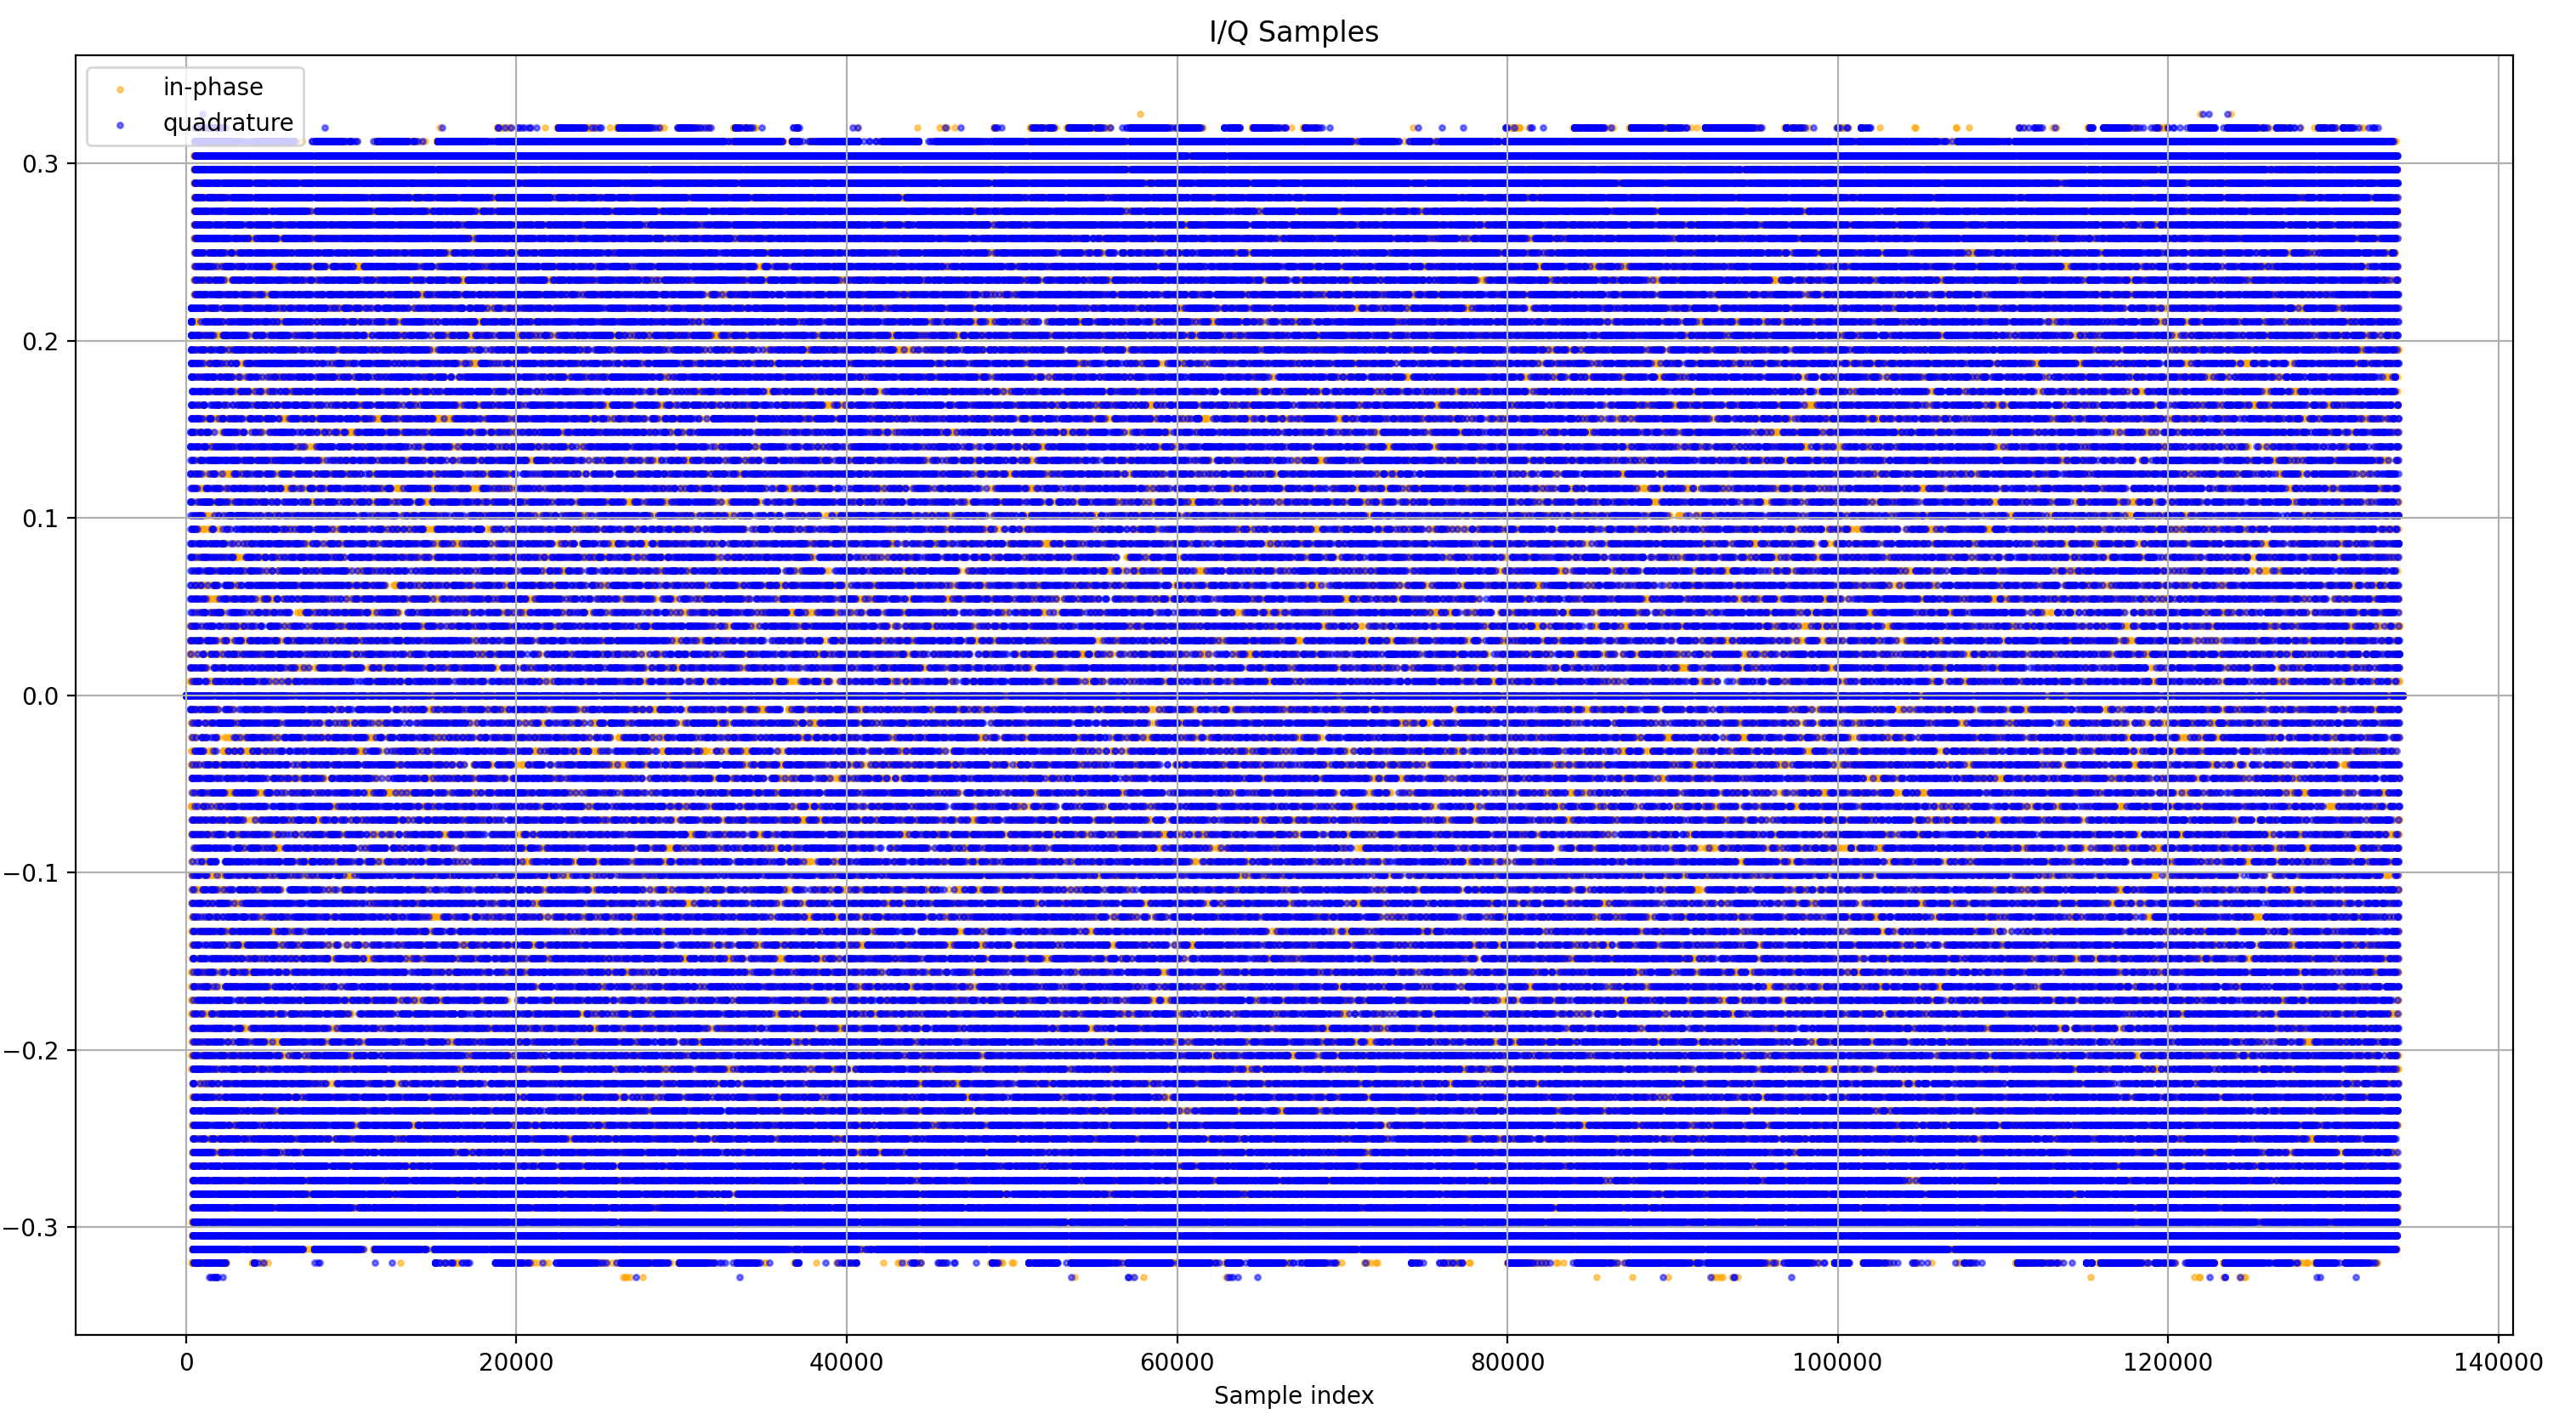
\includegraphics[scale=0.13]{images/iq1.png}
\caption{Plot des échantillons I/Q avec matplotlib}\label{term309}
\end{figure}



\newpage

\begin{figure}[h]
\centering

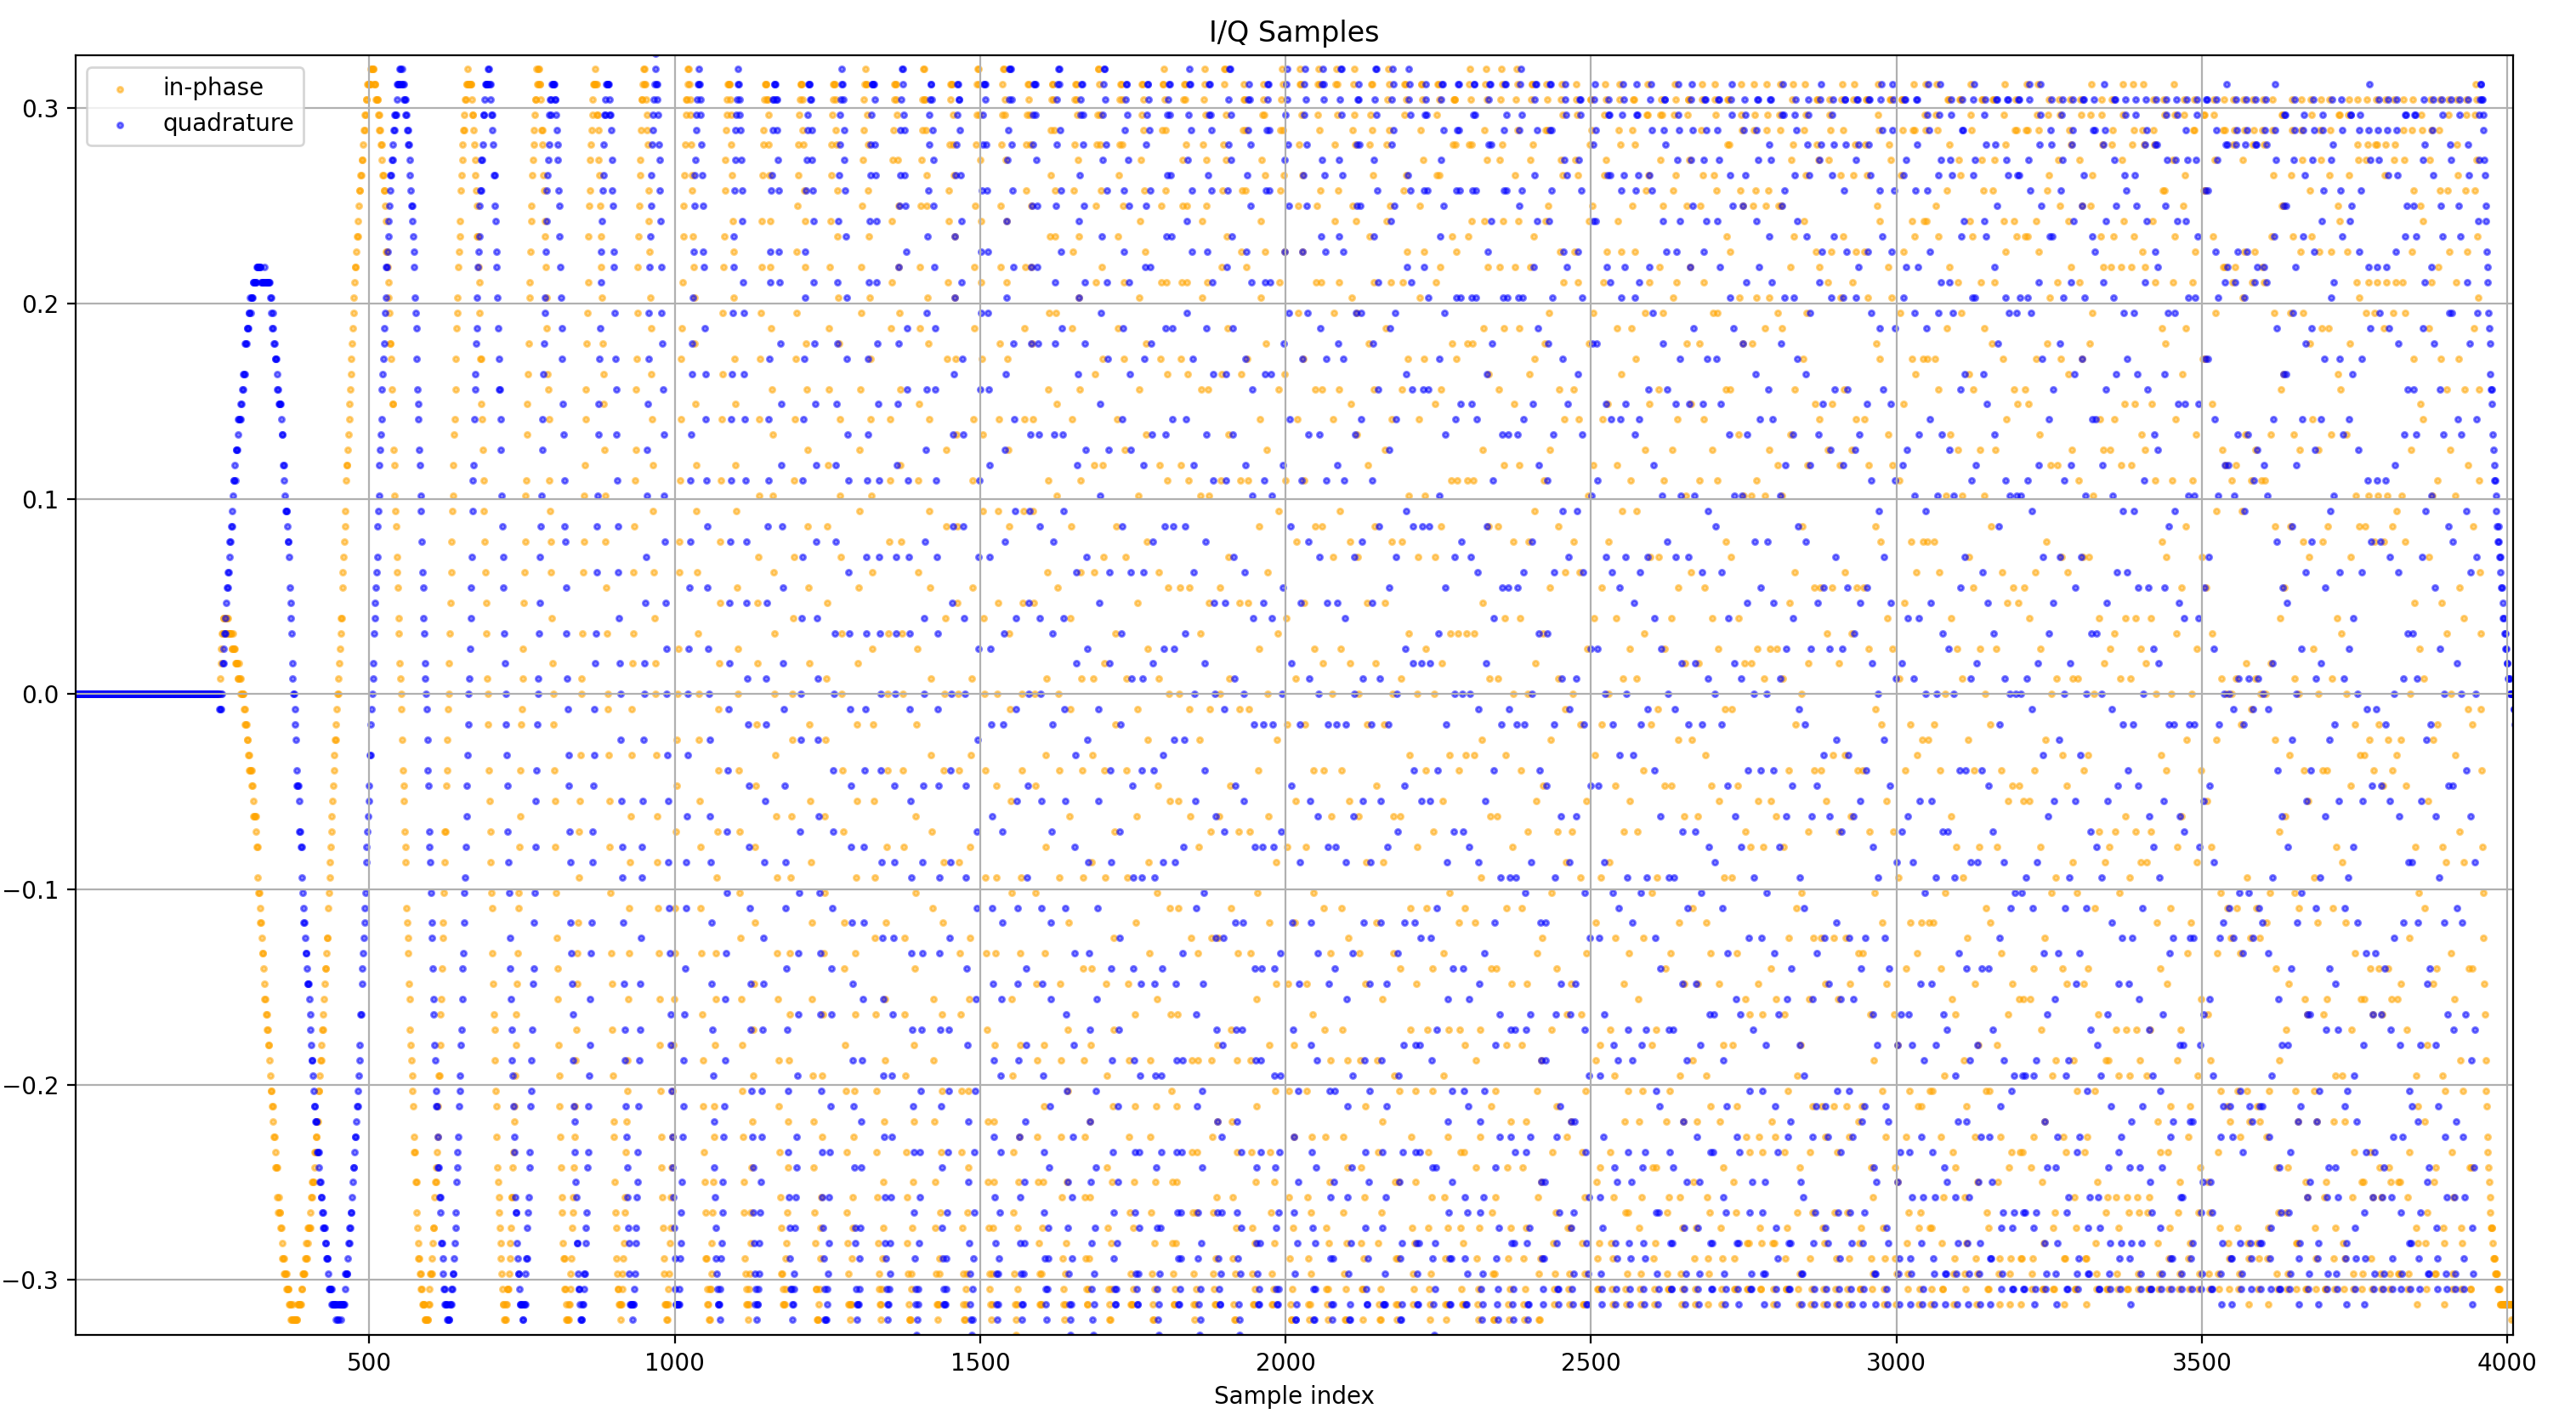
\includegraphics[scale=0.13]{images/iq2.png}
\caption{Zoom sur les 4000 premiers échantillons I/Q}\label{term310}
\end{figure}

\subsection{Automatisation du signal et preprocessing}

Afin de pouvoir effectuer l'identification des appareils, il faut que l'environnement de test soit identique pour chaque module, donc tous les paramètres d'émission sont identiques. La même \ac{SDR} est utilisée avec les mêmes paramètres de réception pour les mêmes raisons. Avec des paramètres d'émission et de réception fixes, il est possible d'automatiser le processus d'enregistrement d'échantillons \ac{LoRa}.

La librairie PyRTLSDR permet de configurer la radio logicielle depuis un script Python (voir annexe \ref{antenne}). La partie du signal que l'on cherche à conserver est le préambule (soit les 8 premiers chirps fixes ou les 12.25 premiers chirps). Si le taux d'échantillonnage est fixe et que le préambule est toujours de la même taille, alors il est possible de calculer le nombre d'échantillons à capturer. 

Par exemple, la figure \ref{term311} indique qu'un préambule complet (12.25 chirps) contient environ 49,000 échantillons. Sachant que le taux d'échantillonnage est de 2MHz pour cet exemple, alors le \ac{TOA} du préambule vaut :

\begin{align}\label{toa}
    Time On Air (TOA) = \frac{N_{samples}}{sample rate} = 0.0245
\end{align}

\clearpage

\begin{figure}[h]
\centering

\includegraphics[scale=0.14]{images/iq3.png}
\caption{Préambule LoRa (sample rate = 2MHz)}\label{term311}
\end{figure}

Maintenant que la durée de l'enregistrement est calculée, il reste à fixer le moment à partir duquel l'enregistrement commence. La méthode la plus facile est d'implémenter un threshold qui détermine si un signal est reçu durant l'écoute. Voici en résumé comment toute l'opération se déroule :

\begin{itemize}
\item les paramètres de l'émetteur sont configurés. 
\item Dès que l'émetteur est prêt à envoyer un signal, le récepteur commence à écouter.
\item Le récepteur informe l'émetteur qu'il est en écoute, l'émetteur envoie un signal.
\item Grâce au threshold, le récepteur commence à enregistrer le \ac{TOA} du signal dès que le threshold est franchi. L'émetteur est en attente pendant que le signal est enregistré dans un fichier.
\item Le récepteur se remet sur écoute et informe l'émetteur qu'il peut envoyer un nouveau signal.
\end{itemize}

Finalement, il reste une dernière étape avant de pouvoir commencer l'identification des modules. Bien que les prises d'échantillons soient en intérieur avec une faible distance entre l'émetteur et le récepteur (voir figure \ref{term312}), les signaux sont parfois fortement atténués. Il faut donc normaliser les données pour contrer les différences d'amplitude. Les données sont normalisées en utilisant \ac{RMS}. La valeur du \ac{RMS} pour un set $x$ de $n$ données ${x_1,x_2,...,x_n}$ vaut la racine carrée de la moyenne arithmétique des carrés des valeurs soit :

\begin{align}
    x_\mathrm{RMS} = \sqrt{\frac{1}{n}(x_1^2 + x_2^2 + ... + x_n^2}
\end{align}

L'implémentation de l'automatisation et de la normalisation est disponible en annexe \ref{codeauto}. L'application de \ac{RMS} a lieu une fois que les données ont été sauvegardées en fichier. Pour chaque répertoire contenant différents signaux capturés, \ac{RMS} est appliqué individuellement sur chacun des fichiers.

\begin{figure}[h]
\centering

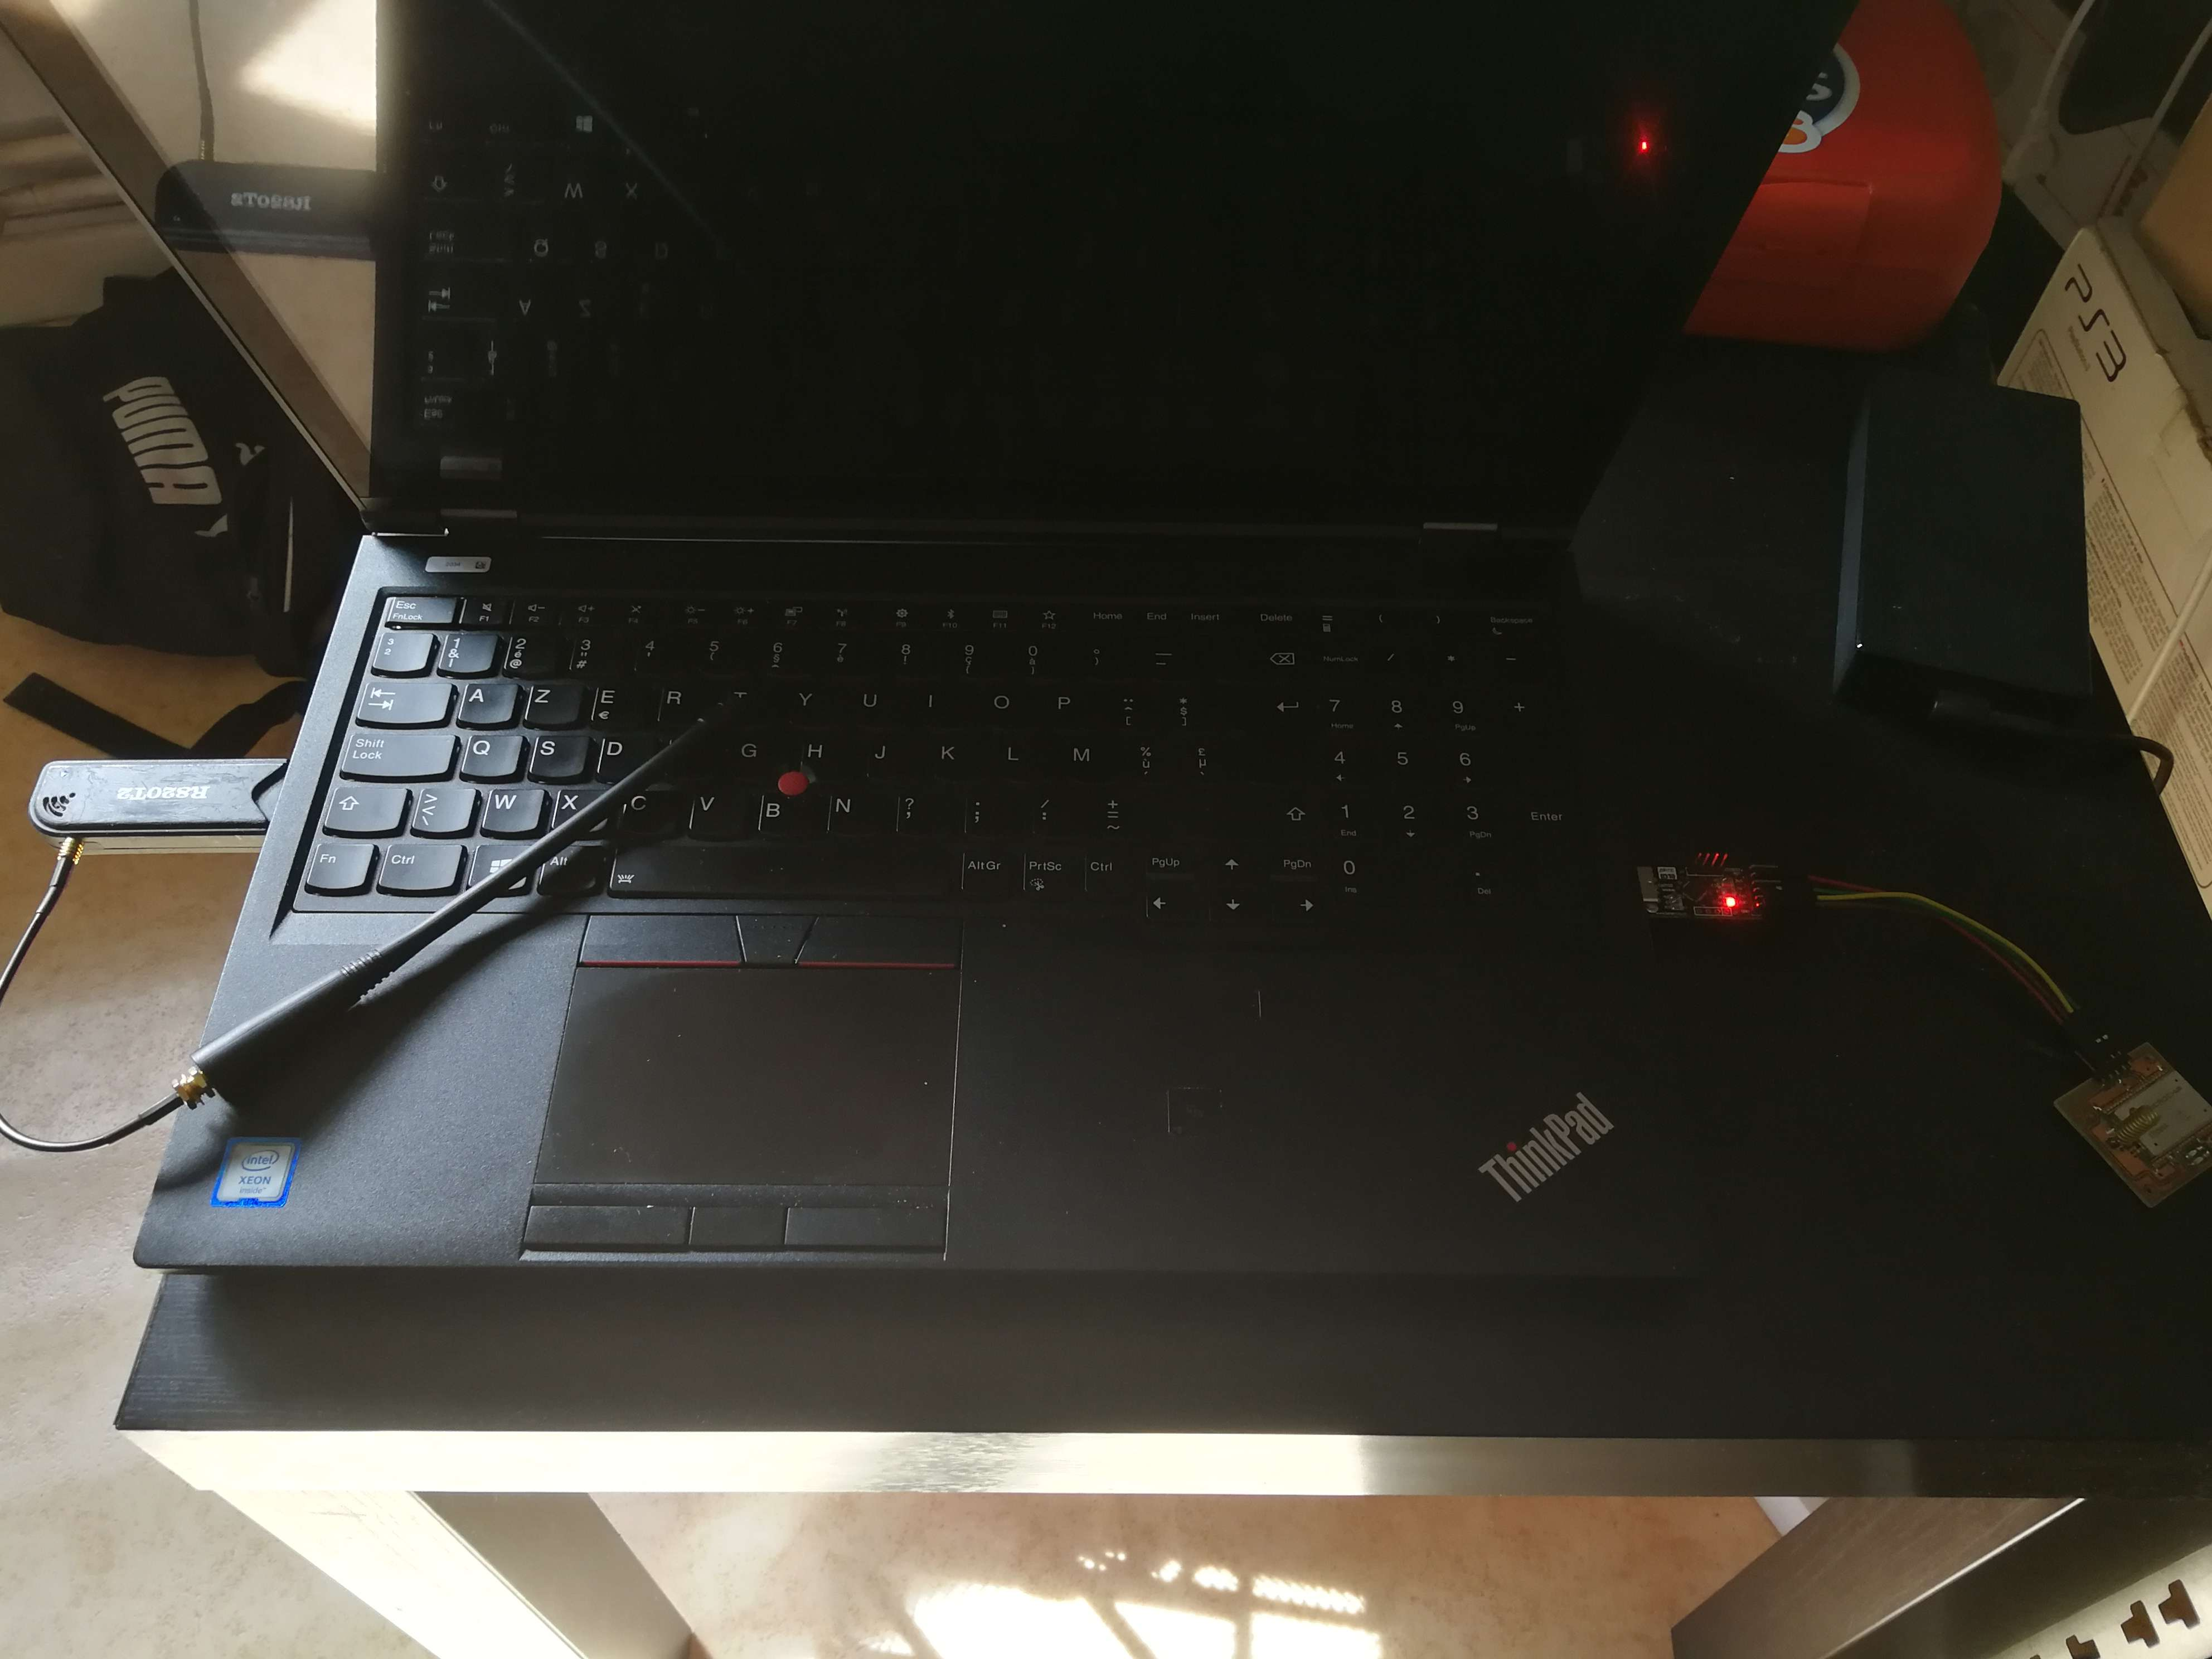
\includegraphics[scale=0.08]{images/conf1.png}
\caption{Configuration en intérieur}\label{term312}
\end{figure}

\chapter{Expérimentations}


\renewcommand{\leftmark}{EXPERIMENTATIONS}

\section{Matériel}

\subsection{radio logicielle}

La radio logicielle ($SDR$, pour $Software$-$Defined Radio$) est une technologie qui permet de mettre en œuvre des systèmes de radio à l'aide de logiciels plutôt que de matériel. 

Dans les systèmes de radio traditionnels, les différentes fonctions de la radio, comme l'accord sur une fréquence spécifique, la modulation et la démodulation du signal, et le filtrage du bruit, sont mises en œuvre à l'aide de composants matériels tels que des oscillateurs, des amplificateurs et des filtres. En revanche, les systèmes SDR utilisent des logiciels pour effectuer ces fonctions, ce qui les rends beaucoup plus flexible car chaque composante est reconfigurable. Les radios logicielle sotn capable d'opérer sur une large portée de fréquence, aussi bien très basse fréquence comme haute fréquence.
Les $SDR$ peuvent jouer le role d'éméteur ou de récepteur voir les deux.

\subsubsection{RTL SDR dvb T}

La première radio utilisée comme récepteur. possède différente composante :

rtl2832U: digitalise les signaux RF et les evnoie à l'ordinateur.
Tuner chip : le tuner permet d'ajuster la fréquence. Grace à ça la sdr peut couvrir une larger portée.
port usb : pour raccorder la sdr à l'ordinateur.

\subsubsection{RTL-SDR R820T2}



meilleure qualitée



\subsubsection{hackRf}

autre radio logicielle. plus (cher et) complète. meilleure qualité de signal que les rtl-sdr "classiques".

\subsection{Module d'émission Lora}

\subsubsection{module RN2483}

Le microchip RN2483 est un module de technologie spécifique à LoRa. Cet appareil permet de communiquer à longue portée et à faible coup grêve à l'utilisation de la modulation basé sur LoRa.

quelques spécificités du module :

technologie LoRa
faible puissance (ideale pour de l'iot car faible consommation)
fréquence à 433, 868 et 915MHz (regarder la régions adéquate)
AT command : configurable via un set de commande
compatible avec le protocole LoRaWAN pour établir ou rejoindre ce type de réseau.

fonctionne par entrée de commande (aucun retour écran donc aucune faute possible)

différentes commandes/ utilisation :

sys get ver : demande la verion du module, reçoit en réponse 
radio set (param) (value) : ajuste le paramètre pour l'adapter a la valeur souhaitée.

\subsubsection{pycom lopy}

besoin  d'un environement python , qqs configuration nécessaire.

\subsubsection{module arduino}

besoin d'un IDE arduino, possibilité de configurer une largeur de bande bien plus faible que pour les autre module, très pratique pour analyser le signal en détail.

\subsection{logiciel}

\subsubsection{gqrx}

logiciel open source d'analyse de fréquence radio pour les SDR.

installer gqrx via apt. (ubuntu)

sélectionner le périphérique pour analyse

\textcolor{red}{image choix périphérique}

visualisation du spectre

deux forme d'affichage,en spectre et en cascade.

L'affichage du spectre fournit une représentation graphique en temps réel du spectre RF sur une gamme de fréquences.
Il montre la puissance du signal de différentes fréquences sur une plage de fréquences spécifiée.
L'axe des x représente la fréquence, tandis que l'axe des y affiche la force du signal (mesurée en dB).

L'affichage en cascade est un spectrogramme qui visualise la force du signal au fil du temps.
Il montre une série d'instantanés de spectre empilés les uns sur les autres, où l'intensité de la couleur représente la force du signal.
Chaque ligne horizontale du tracé en cascade représente une vue du spectre capturée à un moment précis, créant ainsi un enregistrement historique de l'activité du signal.
L'axe vertical représente la fréquence et l'axe horizontal représente le temps.

\textcolor{red}{image affichage spectre}

configuration de la réception :

imput control (pas trop touché)

FFt settings : très important règle la ff size, le raffraichissemetn d'image. le laps de temps. l'averaging

Le paramètre Panadapter dB fait référence à l'échelle verticale dans la vue du spectre. Il représente la force du signal des fréquences radio reçues affichées sur l'axe vertical du graphique du spectre. Le réglage du paramètre Panadapter dB modifie l’échelle verticale de la force du signal affichée dans la vue du spectre.

Le paramètre Waterfall dB concerne l'intensité de la couleur ou l'ombrage des fréquences affichées dans le tracé en cascade.Le réglage du paramètre Waterfall dB modifie l'intensité utilisée pour afficher la force du signal dans le tracé en cascade, permettant ainsi d'ajuster le contraste ou la visibilité des signaux plus faibles ou plus forts.


\subsubsection{Universal radio hacker, URH}

logiciel open source. similaire à gqrx pour fonction d'analyse du signal. Il est possible de visualiser les signaux de manières analogique, démodulé, en spectrogramme ou en vue I/Q. Il est possible de découper les signaux, notamment pour supprimer les parties "vides" dans les enregistrements. Possibilité de sauvegarder des signaux enregistré dans des fichier. Urh supporte différents formats pour les signaux :

 \textit{.complex} files with complex64 samples (32 Bit float for I and Q, respectively). This is the default signal file format.
 
\textit{.complex16u} using two unsigned 8 Bit integers for I and Q

\textit{.complex16s} using two signed 8 Bit integers for I and Q

\textit{.complex32u} using two unsigned 16 Bit integers for I and Q (since v2.7)

\textit{.complex32s} using two signed 16 Bit integers for I and Q (since v2.7).

Il est également possible de lire des fichiers de données qui n'ont pas été enregistré avec URH tant qu'ils sont dans les formats supportés.

\section{Librairie python}

utilisation de python : pourquoi ?
librairie très utile dans le domaine comme NumPy, Pandas, Scikit-learn, PyCM et FiPy.
Librairie disponible pour les radio logiciel hackrf et rtlSDR.
Librairie compatible avec la sauvegarde et l'utilisation des données. Bonne documentation notament sur les formats des nombres complexes.
Capacités pour le machine learning. Utilisation de diverses algorithmes comme kmeans déja implémenté dans des librairies.
Intégration avec des modules, la librairie fipy gère l'un es modules utilisé pour les éxpérimentations.

numpy : pour complexe conjugué
matplotlib : pour les plot des diagrammes
datashader : pour la coloration du diagramme de constellations


\section{Géneration et réception d'un signal LoRa}

dans un premier temps les signaux sont généré manuellement sans automatisation, le but étant de reconnaitre et d'analyser la structure d'un signal Lora. le premier signal est généra via le module rn2483. La documentation est disponible au lien suivant (lien). Via python, il est possible d'utiliser la librairie \textit{Serial} pour se connecter au port usb reliant le module à l'ordinateur. Ensuite, via les différentes commandes, on configure le module en modifiant les paramètres suivant : 

\begin{itemize}
\item la modulation, en LoRa.
\item la fréquence. 868MHz, la fréquence de la bande ISM , la bande d'émission en Europe.
\item la largeur de bande. Dans un premier but de visualiation, on souhaiterai que le message soit le plus long possible dans le temps pour pouvir l'observer facilement. Ainsi la largeur de bande choisie est de 125Khz, ce qui est la plus petite possible valeur que permet le module.
\item la puissance du module, au maximum (14W).
\item le spreading factor. Même raisonement que pour la largeur de bande, on souhaite que le \textit{time on air} soit le plus long possible, donc la valeur la plus grande possible est choisie (SF = 12)
\item le coding rate. Il y a 4 valeur possible:s 4/5, 4/6, 4/7 and 4/8. Cela signifie que tout les 4 bits seront codé par 4, 5, 6, 7 ou 8 bits de transmissions en fonction de cette valeur. Plus la valeur st faible (la plus faible étant 4/8), plus le time on air sera élevé, car cela prend plus de temps pour transmettre le message.
\end{itemize}

Les commandes relatives à la configuration sont disponibles en annexes.
Une fois que le module est configurer, il faut paramètrer le recpeteur, la radio logicielle. La librairie pyrtlsdr permet de pouvoir configurer le récepteur, elle sera utlisée pour les expérmientations dans la section 3.4. Dans un premier temps, les logiciels comme gqrx ou urh permettent également de pouvoir configurer le récepteur. Leur utilisation a déja été décrite dans la section 3.1.3. Les paramètres à configurer sont les suivant : 

\begin{itemize}
\item la fréquence. La fréquece d'écoute. Idéalement la même fréquence de celle de l'émetteur (868MHz). Cependant celle ci sera légèrement décalée pour contrer un effet
\item le taux d'échantillonage. Il est possible de choisir la quantitté d'échantillons traitée chaque seconde. Un taux plus élevé donnera un signal plus complet. Le taux minimal ne doit jamais être inférieur à deux fois la largeur de bande. (Théorème de nyquist shannon : fe > 2fmax)
\item le gain. Dépendant de la qualité du signal il peut être nécessaire d'ajouter du gain, c'est à dire d'amplifier la force du signal. Un gain trop élevé peut saturer le signal, quand l'amplitude dépasse la portée du récepteur.
\end{itemize}

Une fois l'émetteur et le récepteur configuré, il est maintenant possible de visualiser des signaux Lora.

\subsection{analyse avec gqrx}



\subsection{analyse avec urh}

affichage du signal capturé, d'abords sous forme analogique, puis en spectrogramme.
Décomposition du signal, on observe des "chirps". En analogique, augmentation de la fréquence (unchirp) et diminution de la fréquence (downchirp). En spectrogramme, augmentation est plus visuelle encore, on voit de manière net les chirps.

Dans le signal, on reconnait donc le préambule du signal composé de 10 upchirps et 2 downchirps (selon la théorie).

Attention, la fréquence d'écoute des sdr ne doit pas être exactement à 868Mhz. En effet, voilà à quoi ressemble si la fréquence d'écout est la même que la fréquence d'émission. Il faut prendre en compte la largeur de bande du signal, dans le cas ou le singal a une largeur de bande de 125KHz, il faut décaler la fréquence d'écoute pour recentrer le signal, ainsi on évite d'avoir des fréquence qui sont interprétée comme "négatives" par URH. Dans la figure, la fréquence est décalé de 125/2 soit 867,935Mhz.

\subsection{automatisation du signal et preprocessing}

Dans un second temps, besoin d'automatiser la génération et l'enregistrement des signaux afin de pouvoir travailler avec un grand nombre d'échantillons. La librairie python pytlsdr permet de ne pas devoir passer par un logiciel comme urh pour sauvegarder les échantillons. La méthode d'enregistrement est la suivate :

\begin{itemize}
\item d'abords, configurer la module et la rtlsdr avec les différent paramètre
\item ensuite l'antenne commence a enregistrer. L'émetteur est informé que la radio logiciel est en écoute et envoie un signal. 
\item dès que la radio reçoit le signal, elle informe l'émetteur de se mettre en attente car le preprocessing commence.
\item Le signal reçu est découpé pour ne conserver que le preambule, et puis enregistrer dans un fichier.
\item dès que l'enregistrement est terminé, le cycle recommence.
\end{itemize}

la code source est disponible en annexe.


\section{Méthode "Constellation traces"}

objectif, identification du device via son frequecy offset.

selon l'article (citer article), possible de performer la méthode soit uniquement sur le  préambule, soit sur l'intégralité du singal. 

idée: le received singal contient le baseband singal ainsi qu'un rotation factor instable. pour pouvoir recover cette partie du signal, besoin d'effctuer une opération différentielle suivante : $$ x(t) . x(t+n) e -j2\pi on $$
apparation d'un nouveau rotation factor, mais stable. Besoin de trouver deux inconnue,\textit{delta f} et \textit{n}. n est le differential interval. il se calcule de la manière suivante : $$ Rs = BW / 2sf $$ 
$$ N = fs / Rs $$

delta f est la difference entre le transmitter carrier frequency et le receiver carrier frequecy.

application : récupérer les samples I/Q du signal n ayant au préalable "clean" le signal. utilisation d'un gradiant pour observer la dentsité sur le plot. noramlement des zones plus denses apparaissent.
coloration : utilisation de la librairie data shader. 


clustering, le but de conserver les parties les plus dense (95pourcent du point le plus dense) plot avec les différents appareils.
librairie panda et numpy. découpage en zones (bins?) sous forme d'une grille, calcul de nobre de points dans chaque zone, la zone avec le plus grand nombre de point sers de maximum. 



\chapter{Résultats}

\include{chapters/coclusion}


\bibliographystyle{latex8}
\bibliography{biblio}

\newpage
\appendix
\addcontentsline{toc}{chapter}{Annexes}

\chapter{Premi\`ere annexe}
\renewcommand{\leftmark}{ANNEXE \thechapter.~~Premi\`ere annexe}
\label{annexe1}

\chapter{Deuxi\`eme annexe}
\renewcommand{\leftmark}{ANNEXE \thechapter.~~Deuxi\`eme annexe}
\label{annexe2}

%%%%%%%FIN-ANNEXES%%%%%%%%%%
\end{document}
